This appendix presents more details on the measurement of the data-driven real lepton efficiency using the $Z$ tag-and-probe method.

%%%
%%%
%%%

\section{The $Z$ tag-and-probe method}
\label{sec:app_RLE_ZTandP_method}
The $Z$ tag-and-probe method is used to extract the leptons from data and measure the real lepton efficiency.
The selected events are required to have at least two baseline leptons.
The lepton candidates with $\pt > 25$~{\GeV} and satisfying all the signal lepton requirements are categorized into \textit{tag leptons}.
The lepton candidates passing baseline lepton requirements can be classified as \textit{probe leptons}.
In order to form a tag-and-probe pair, the two selected leptons have to carry the same flavor and opposite charge.
The invariant mass of the tag-and-probe pair system should satisfy the $Z$ boson mass window $80 < m_{\ell \ell} < 100$~{\GeV}.
All possible combinations of the tag-and-probe pairs are considered to avoid any bias and to increase the statistics.
For the $Z \to ee$ decay, an additional $|\eta| < 2$ requirement is applied on the tag and probe leptons.
However, no additional requirement is applied for the $Z \to \mu \mu$ decay.
The tag lepton is used to select the probe lepton only and the probe lepton is used for the real efficiency measurements.
In this study, the tag and probe leptons are required to match the lepton triggers listed in Table~\ref{tab:app_RLE_single_lepton_triggers}.

\begin{table}[htbp]
    %\begin{center}
    \resizebox{\textwidth}{!}{% <------ Don't forget this %
        % {\footnotesize
            \begin{tabular}{llll}
                \hline
                \hline
                Trigger                                & lepton   & 2015                                     & 2016\\
                \hline
                \multirow{2}{*}{Single lepton trigger} & electron & \texttt{e24\_lhmedium\_iloose\_L1EM20VH} & \texttt{e26\_lhtight\_nod0\_ivarloose}\\
                                                       & muon     & \texttt{mu20\_iloose\_L1MU15}            & \texttt{mu26\_ivarmedium}\\
                \hline
                \multirow{2}{*}{Dilepton trigger}      & electron & \texttt{2e12\_lhloose\_L12EM10VH}        & \texttt{2e17\_lhvloose\_nod0}\\
                                                       & muon     & \texttt{mu18\_mu8noL1}                   & \texttt{mu22\_mu8noL1}\\
                \hline
                \hline
            \end{tabular}
        % }
    }
    %\end{center}
    \caption{The list of single lepton and dilepton triggers used for the real lepton efficiency measurements.
    The dilepton triggers are used for studying the systematic uncertainties causing by the trigger.}
    \label{tab:app_RLE_single_lepton_triggers}
\end{table}

Figure~\ref{fig:app_RLE_mll_distributions} shows the data-to-MC comparison of the tag-and-probe pair invariant mass distributions which indicate the need of subtracting the background especially for the probe electron with $\pt < 20$~{\GeV}.
A background template method, which is similar to the one used by the $e/\gamma$ performance group for their efficiency measurements~\cite{ATLAS-CONF-2014-018}, is used to estimate the background contamination from the low \pt electrons.
No background subtraction is performed on the signal leptons because the background contamination is found to be negligible.
However, the background contamination in the baseline probe leptons needs to be subtracted.
The real lepton efficiency is obtained by the following equation
%
\begin{equation}
    \epsilon = \frac{N_{\mathrm{signal}}}{N_{\mathrm{baseline}} - N_{\mathrm{baseline}}^{bkg}}
    \label{eq:app_RLE_efficiency_formula}
\end{equation}
%
where $N_\mathrm{signal}$ is the number of probe leptons passing the signal requirements, $N_\mathrm{baseline}$ is the number of probe leptons passing the baseline requirements, and $N_\mathrm{baseline}^{bkg}$ is the estimated background contamination in the baseline probe leptons.

\begin{figure}[htbp]
    \begin{subfigure}[b]{0.48\textwidth}
        \begin{center}
            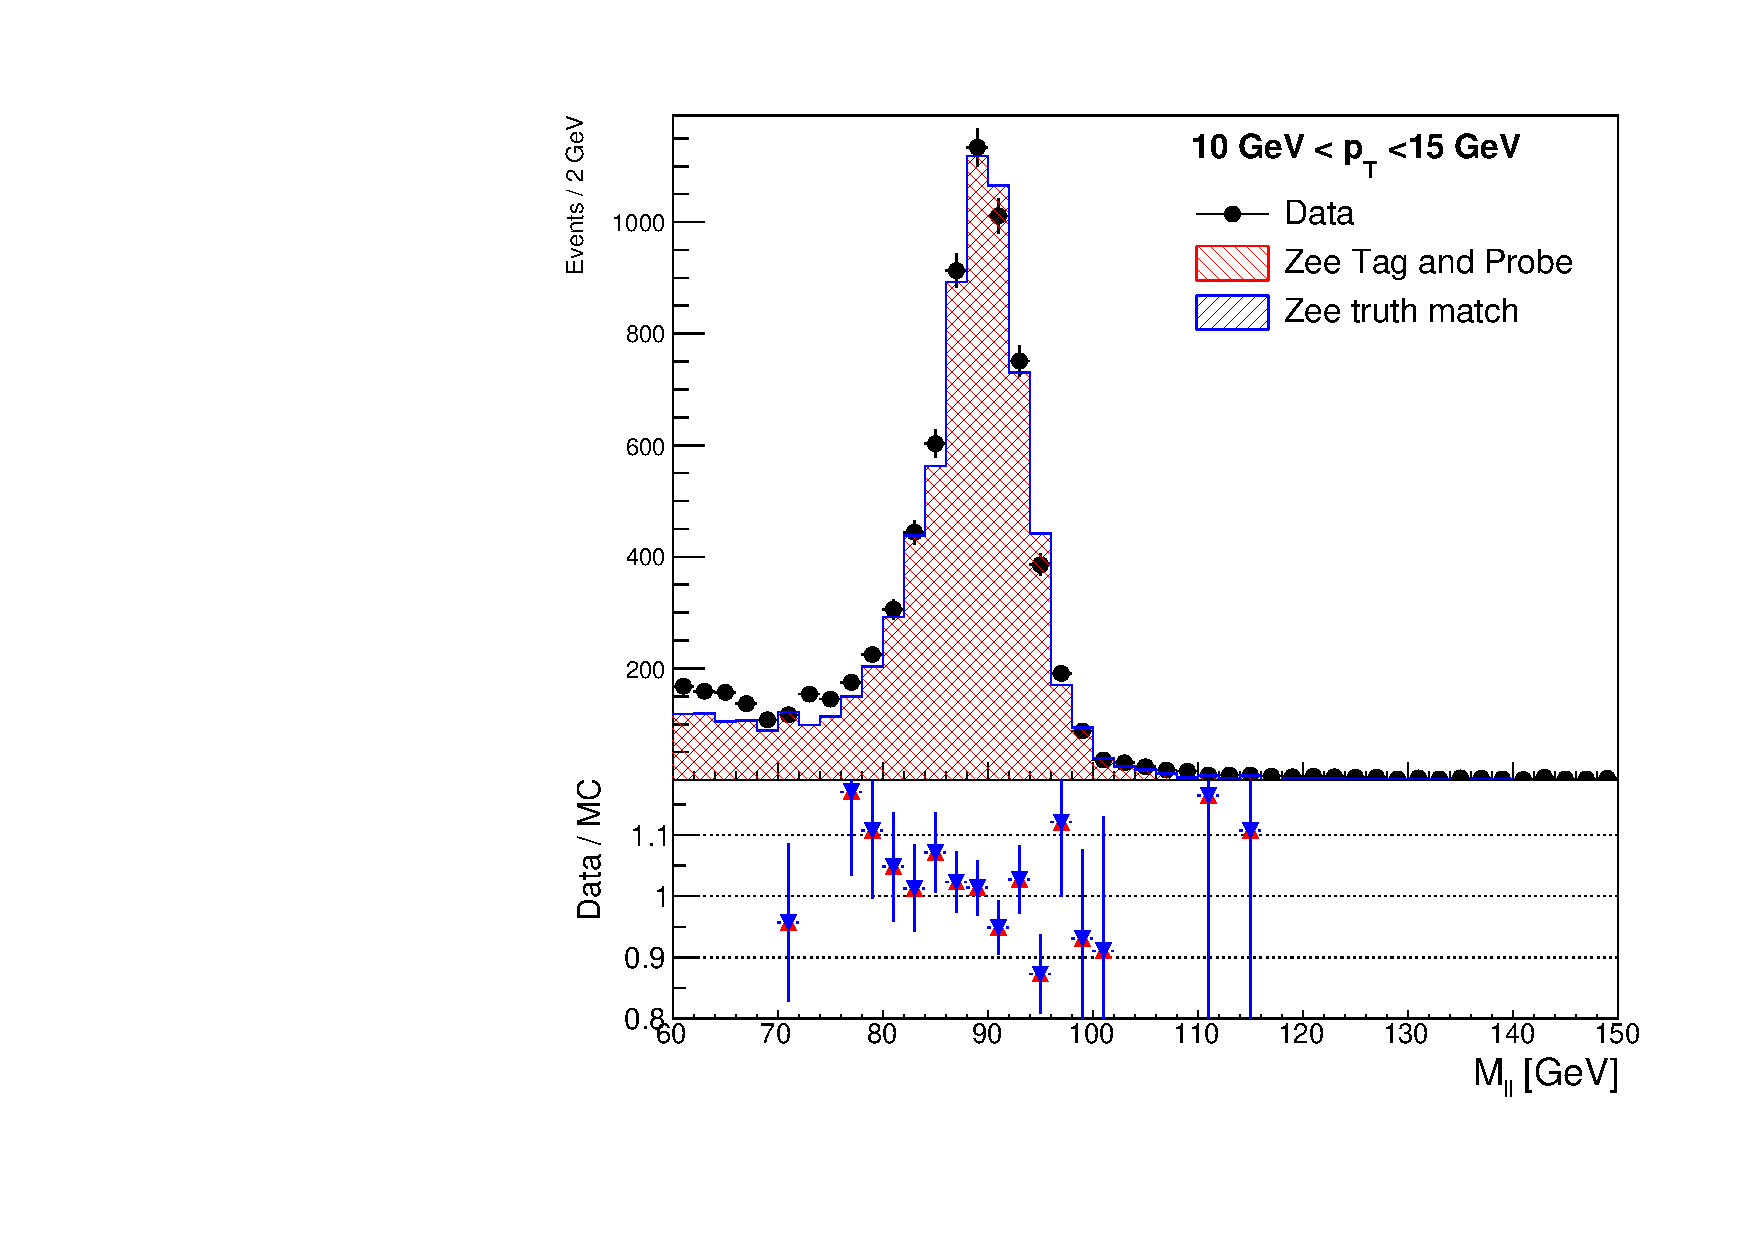
\includegraphics[scale=0.35]{signal_level_Mee_pt1015_ratio_plot_MC_normalized.pdf}
            \caption{The $m_{ee}$ distribution with $10 < \pt < 15$~{\GeV}.}
        \end{center}
    \end{subfigure}%
    \begin{subfigure}[b]{0.48\textwidth}
        \begin{center}
            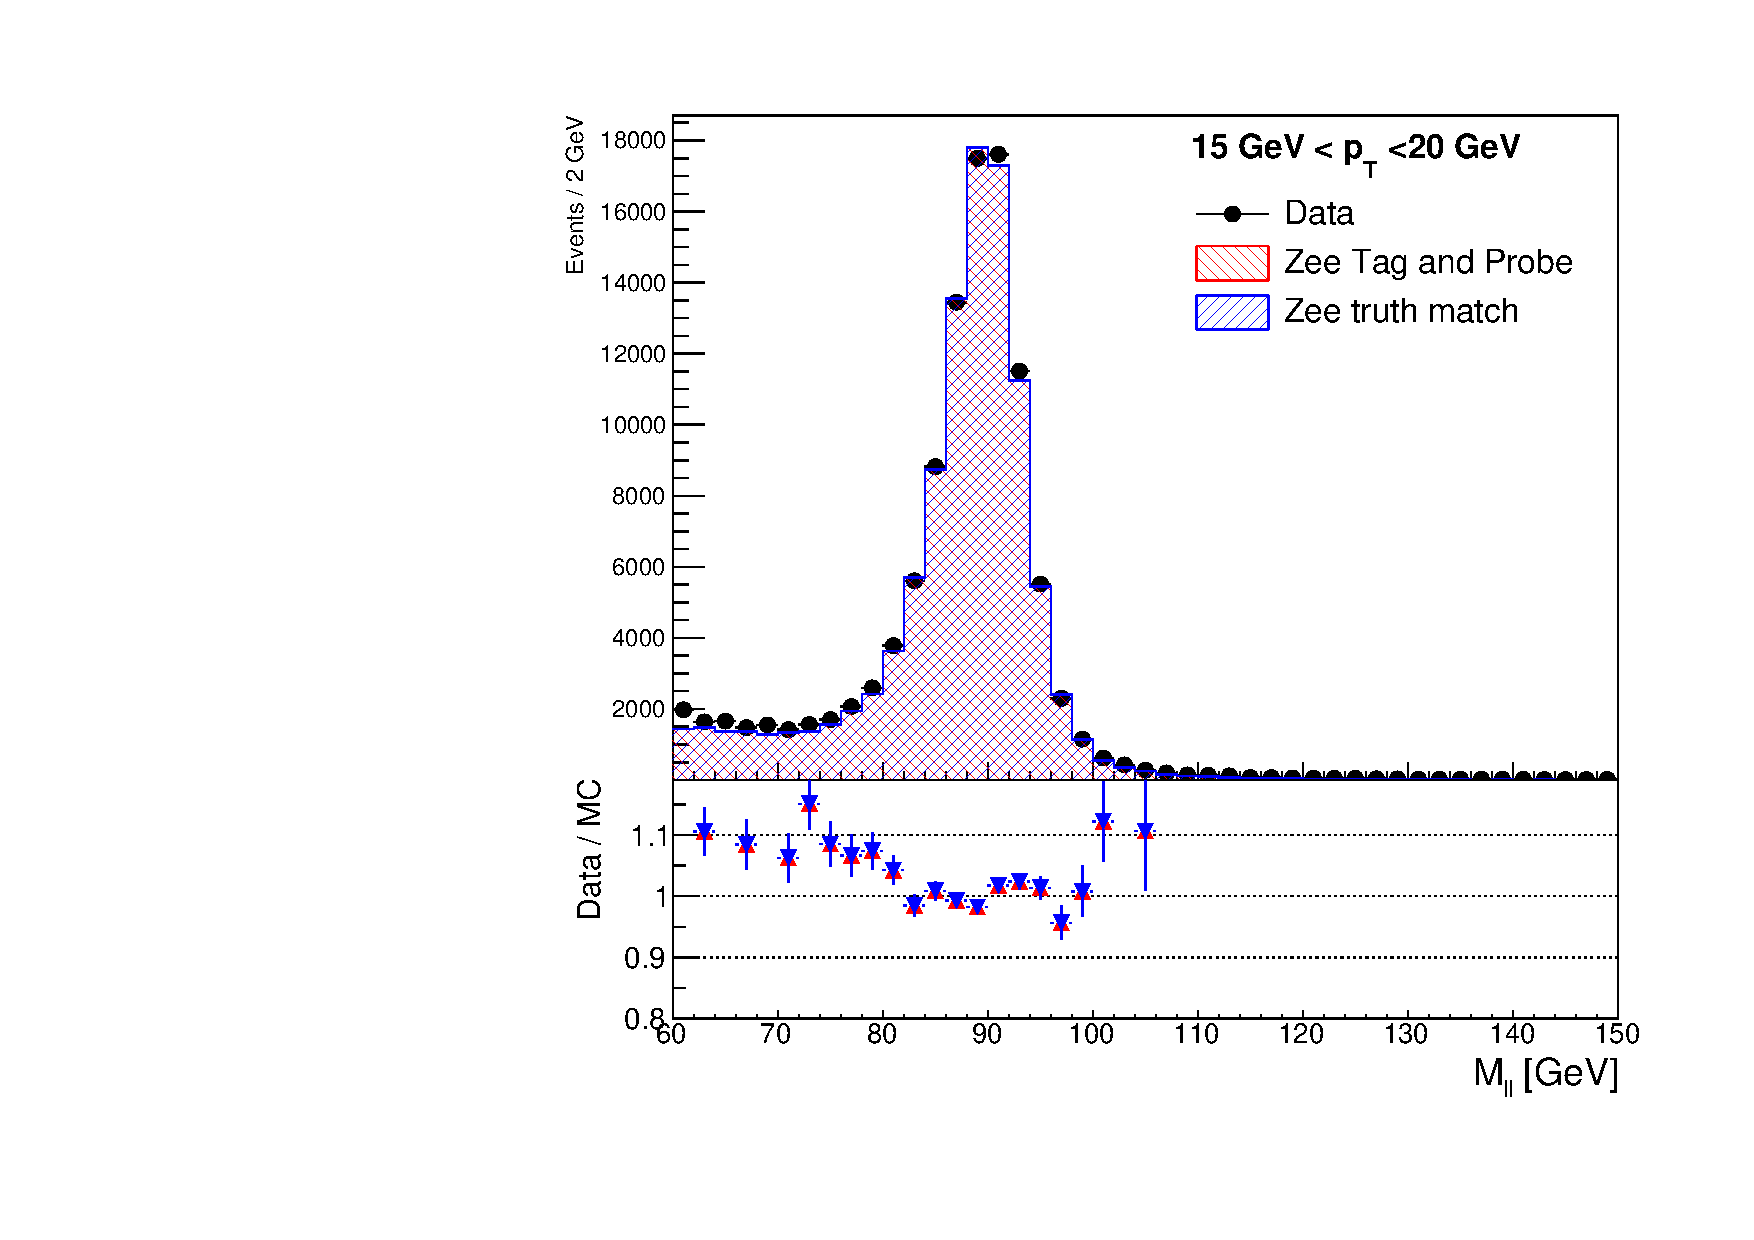
\includegraphics[scale=0.35]{signal_level_Mee_pt1520_ratio_plot_MC_normalized.pdf}
            \caption{The $m_{ee}$ distribution with $15 < \pt < 20$~{\GeV}.}
        \end{center}
    \end{subfigure}
    \begin{subfigure}[b]{0.48\textwidth}
        \begin{center}
            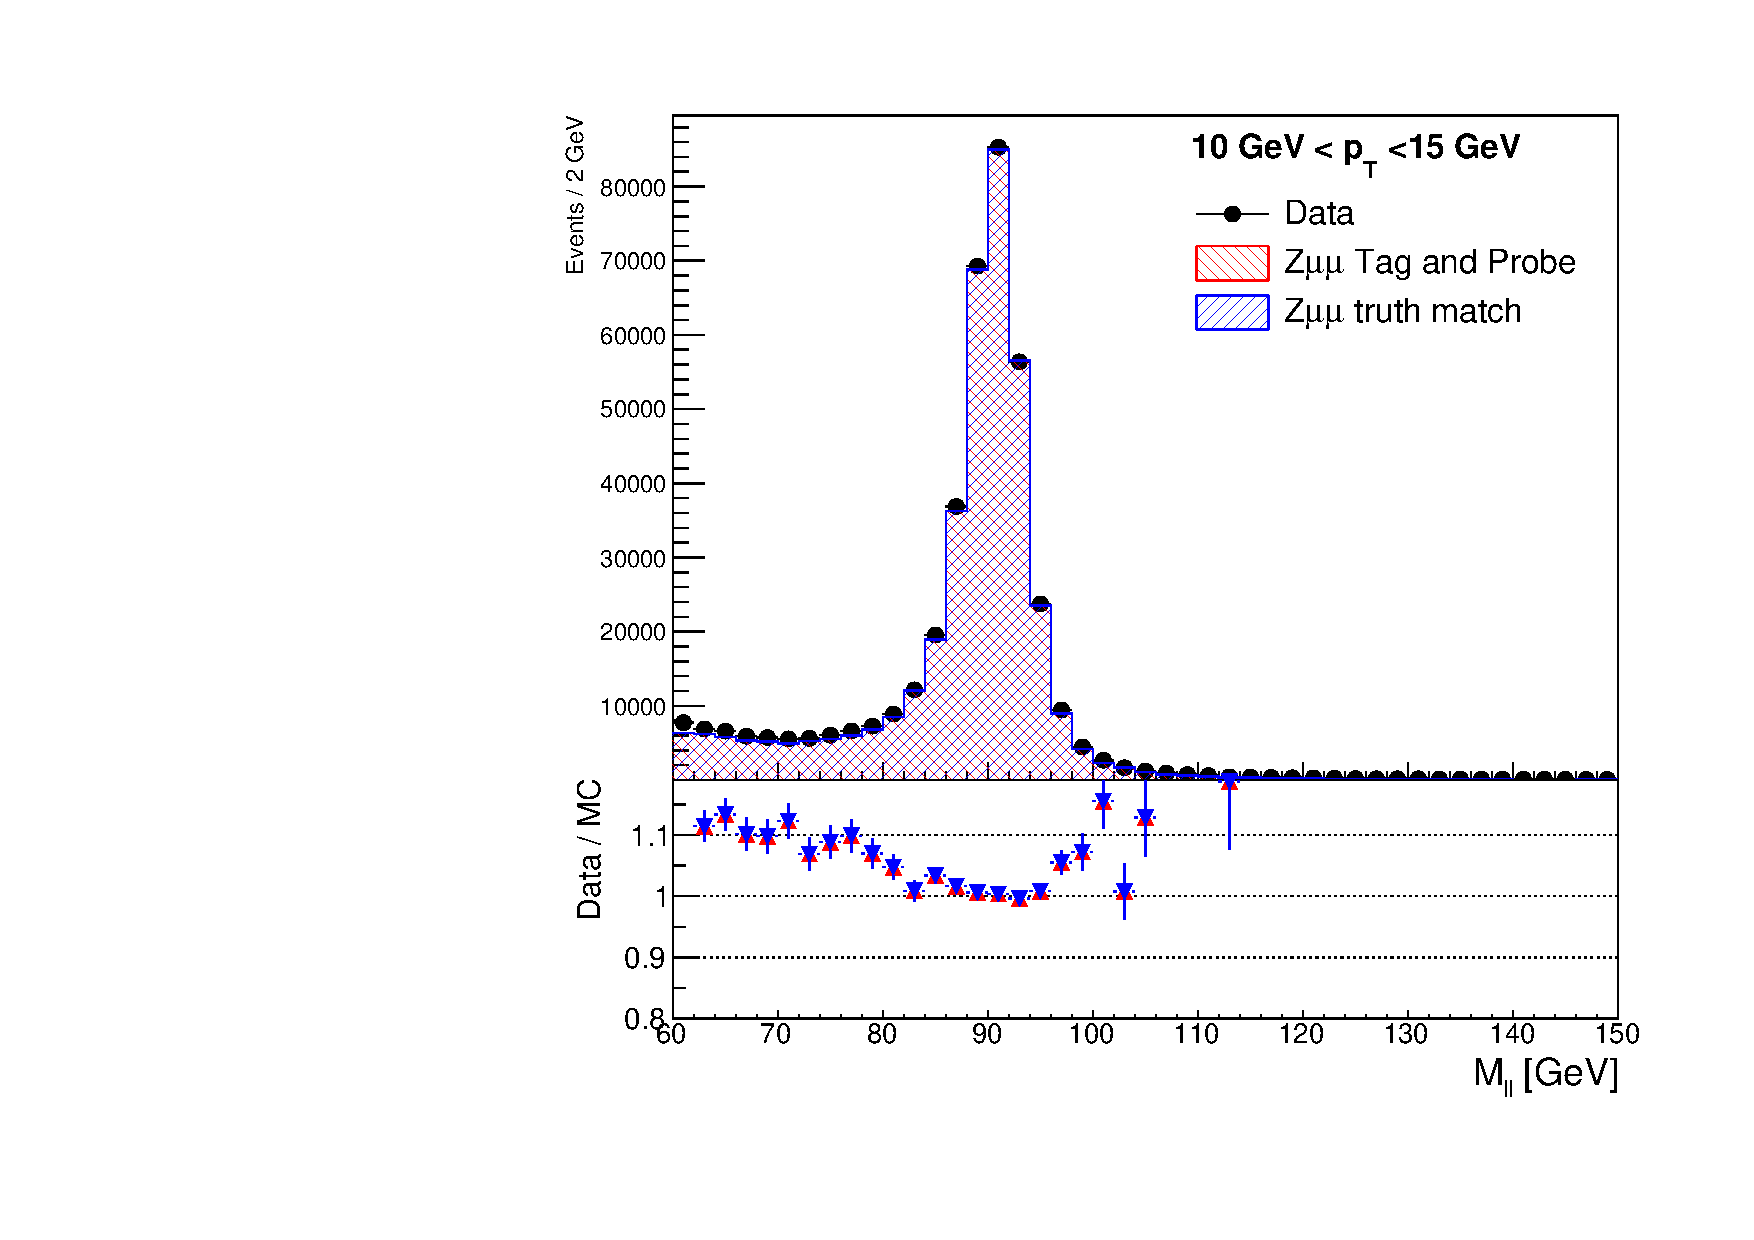
\includegraphics[scale=0.35]{signal_level_Mmumu_pt1015_ratio_plot_MC_normalized.pdf}
            \caption{The $m_{\mu\mu}$ distribution with $10 < \pt < 15$~{\GeV}.}
        \end{center}
    \end{subfigure}%
    \begin{subfigure}[b]{0.48\textwidth}
        \begin{center}
            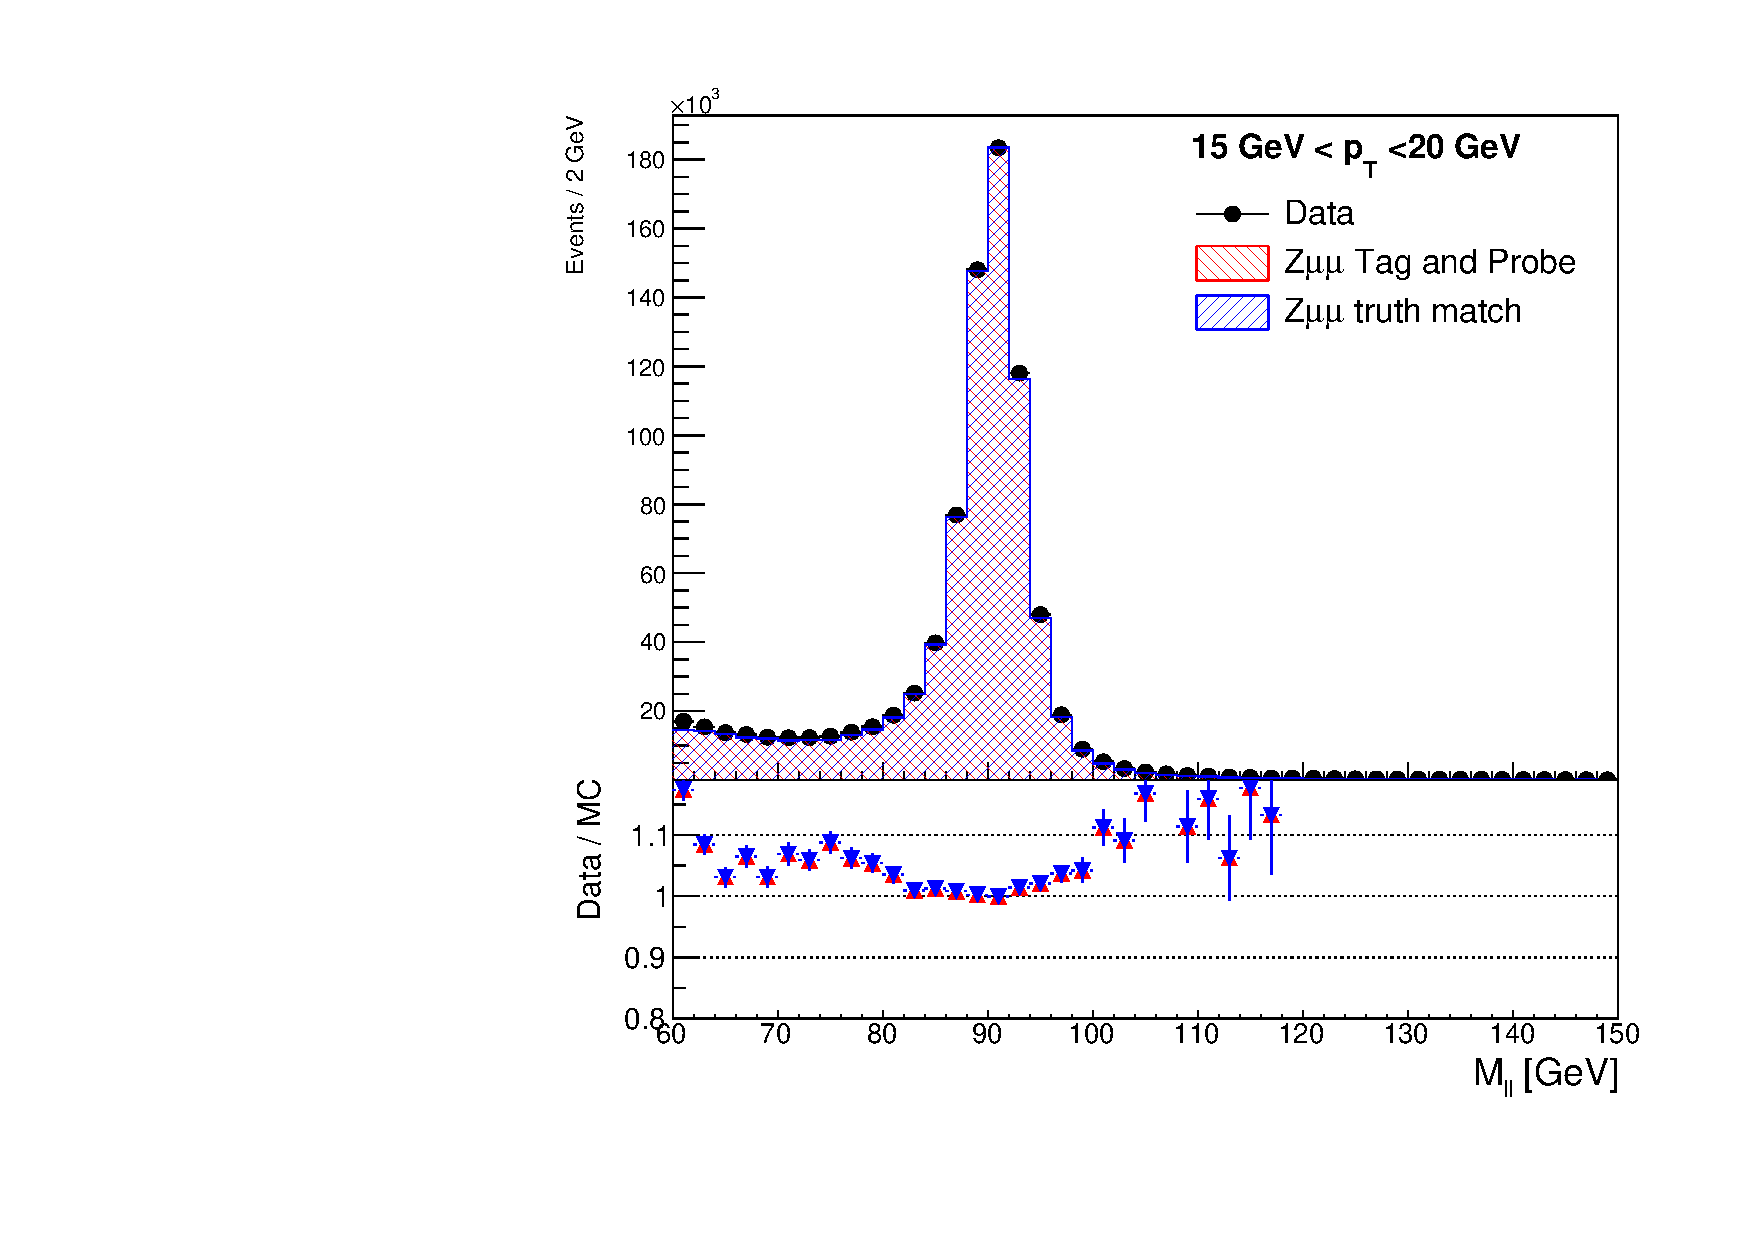
\includegraphics[scale=0.35]{signal_level_Mmumu_pt1520_ratio_plot_MC_normalized.pdf}
            \caption{The $m_{\mu\mu}$ distribution with $15 < \pt < 20$~{\GeV}.}
        \end{center}
    \end{subfigure}
    \caption{The invariant mass distributions of the tag-and-probe pair computed using $Z+jets$ MC and 2015 + 2016 data.
    The red color stands for the $Z$ tag-and-probe events, the blue color represents the $Z$ truth matched events, and the black dots are data.
    The MC distributions are scaled to the data using a Gaussian fit of the $Z$ mass peak $85 < m_{\ell \ell} < 95$~{\GeV}.}
    \label{fig:app_RLE_mll_distributions}
\end{figure}

%%%
%%%
%%%

\section{Background subtraction}
\label{sec:app_RLE_bkg_subtraction}
The background template method is used to evaluate the background contamination on data.
By inverting the calorimeter and track isolations, requesting the electron object to fail the medium LH identification, the background sample enriched template can be obtained.
Three background templates are considered for the systematic study.
The definitions of the background template are summarized in Table~\ref{tab:app_RLE_bkg_templates}.

\begin{table}[htbp]
    %\begin{center}
    \resizebox{\textwidth}{!}{% <------ Don't forget this %
        % {\footnotesize
            \begin{tabular}{cccc}
                \hline
                \hline
                cut                   & variation 1 template                   & baseline template                       & variation 2 template\\
                \hline
                Identification        & -                                      & fail medium LH                          & fail medium LH\\
                Calorimeter isolation & $E_\mathrm{T}^{topocone20} /\pt > 6\%$ & $E_\mathrm{T}^{topocone20} /\pt > 15\%$ & $E_\mathrm{T}^{topocone20} /\pt > 20\%$\\
                Track isolation       & $p_\mathrm{T}^{varcone20} /\pt > 6\%$  & $E_\mathrm{T}^{topocone20} /\pt > 8\%$  & $E_\mathrm{T}^{topocone20} /\pt > 15\%$\\
                \hline
                \hline
            \end{tabular}
        % }
    }
    %\end{center}
    \caption{The definition of the background templates for estimating the background contamination associated with the $Z$ tag-and-probe method.
    The baseline template is used to estimate the background contamination.
    The variation 1 template has looser requirements and the variation 2 template has tighter requirements.
    They are used to assess the systematic caused by the background contamination.}
    \label{tab:app_RLE_bkg_templates}
\end{table}

\begin{figure}[htb]
    \begin{subfigure}[b]{0.48\textwidth}
        \begin{center}
            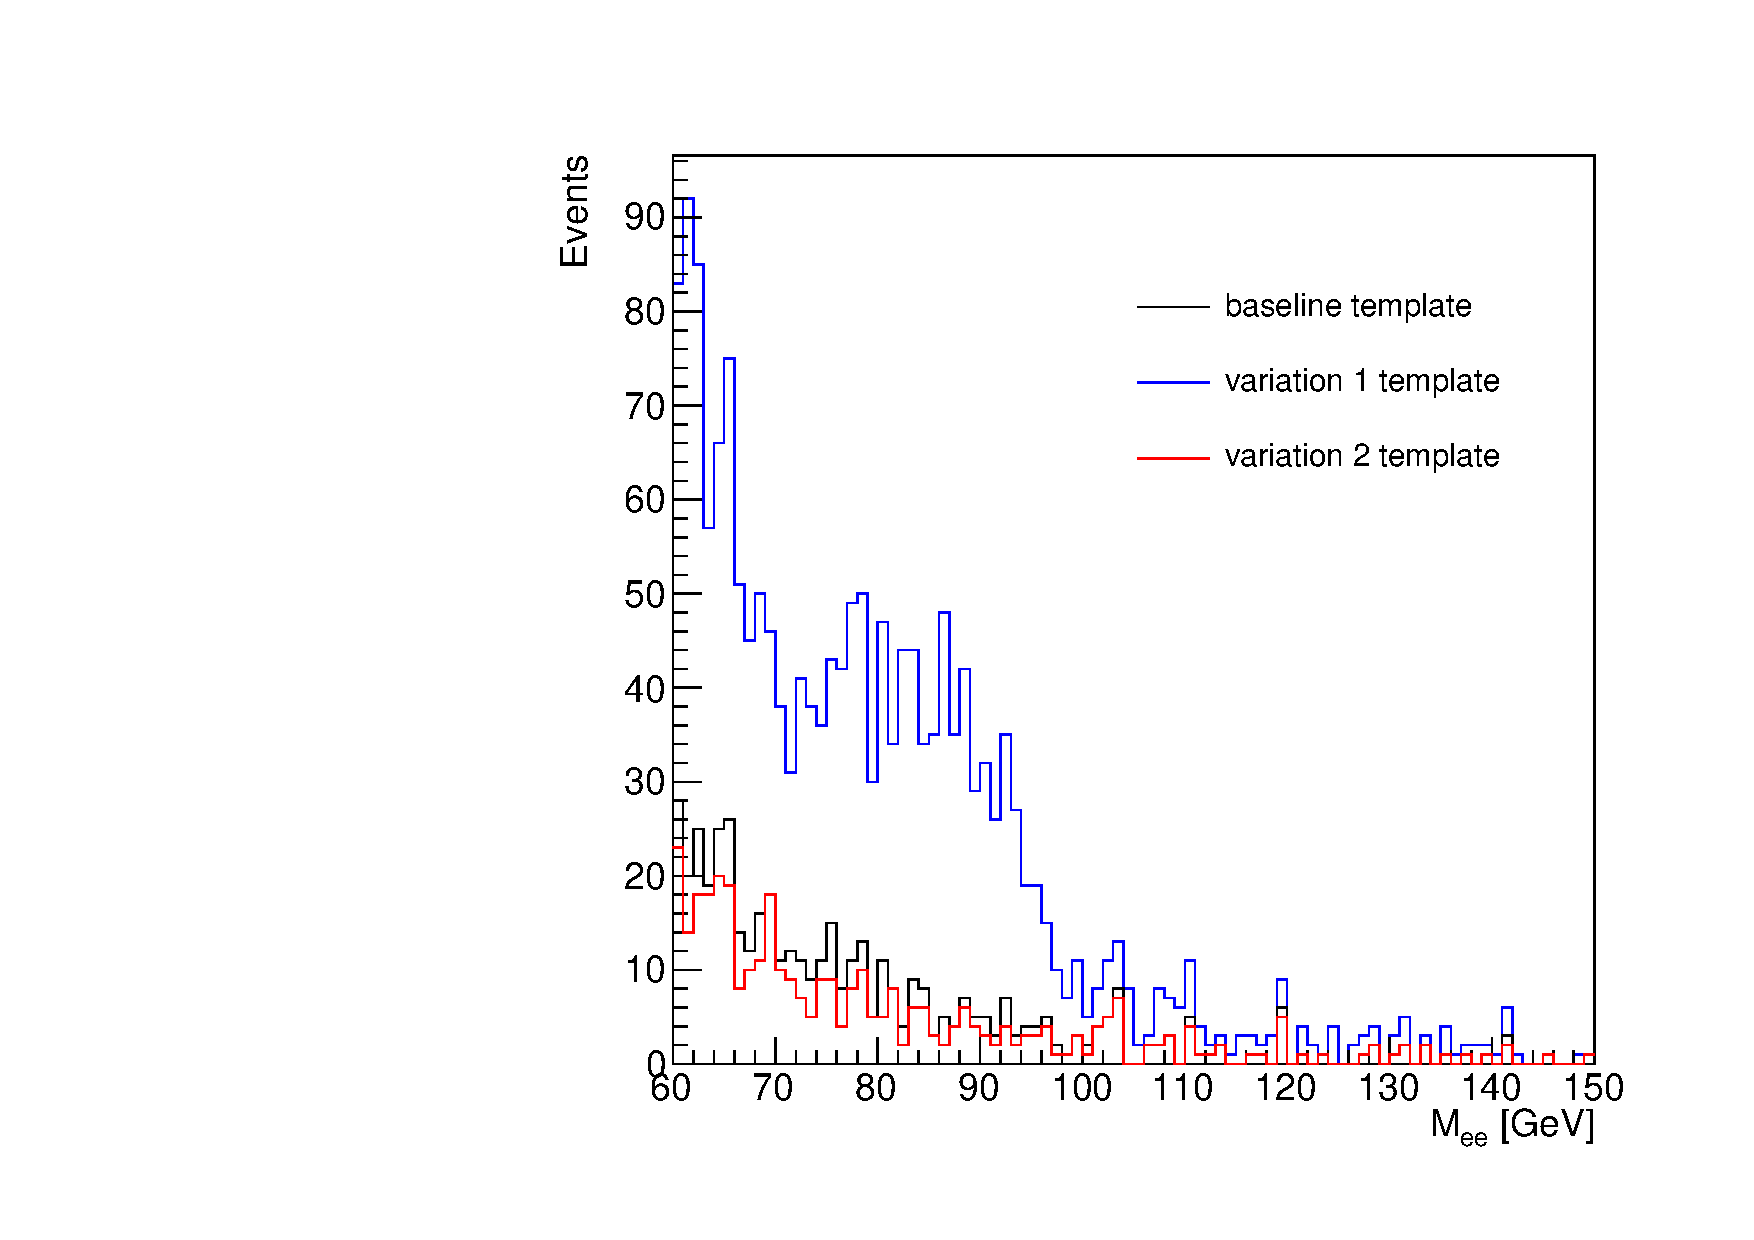
\includegraphics[scale=0.35]{bkg_template_electron_pt_1015_eta0201.pdf}
            \caption{Probe electrons with $10 < \pt < 15$~{\GeV}.}
        \end{center}
    \end{subfigure}
    \begin{subfigure}[b]{0.48\textwidth}
        \begin{center}
            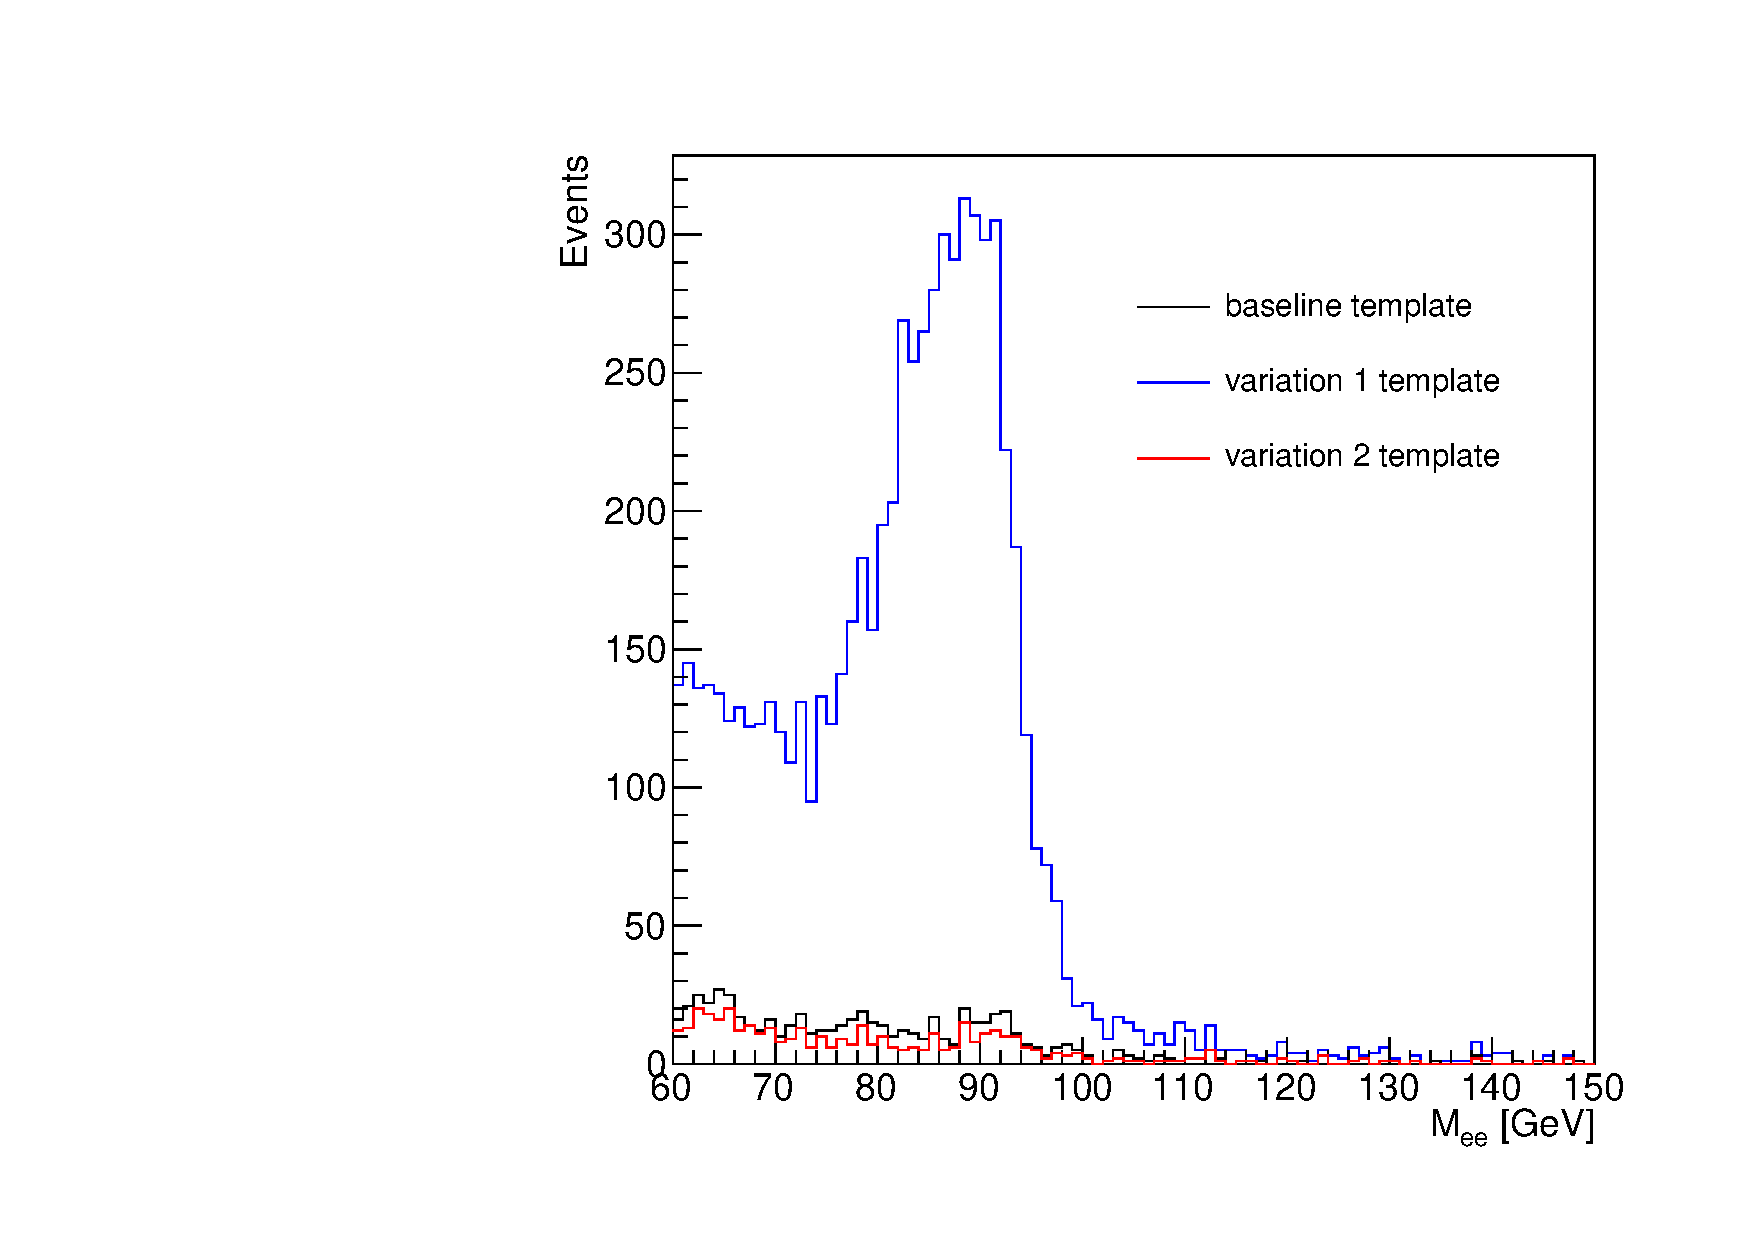
\includegraphics[scale=0.35]{bkg_template_electron_pt_1520_eta0201.pdf}
            \caption{Probe electrons with $15 < \pt < 20$~{\GeV}.}
        \end{center}
    \end{subfigure}
    \caption{The $m_{ee}$ distributions for the baseline, variation 1 and variation 2 background templates.
    The $m_{ee}$ distributions are computed using the probe electrons with different \pt as indicated in the caption of plots.
    The variation 1 template has looser calorimeter and track isolation requirements and the baseline and the variation 2 templates have tighter selection criteria.
    So a peak can be seen in the $Z$ mass region in variation 1 template but not in the baseline and variation 2 templates.}
    \label{fig:app_RLE_bkg_templates}
\end{figure}

Figure~\ref{fig:app_RLE_bkg_templates} shows the $m_{ee}$ distributions of the background template.
The invariant mass distribution of the template events ($m_{ee}^\mathrm{template}$) is then used to estimate the amount of background in $80 < m_{\ell \ell} < 100$~{\GeV} region.
In order to estimate the correct of background events, the $120 < m_{ee} < 150$~{\GeV} region is used to normalize the background template because a smaller prompt electron contribution is expected in this region.
Equation~\ref{eq:app_RLE_bkg_in_the_tail} shows the estimation of the number of background events in the tail region using the baseline electrons.
%
\begin{equation}
    N_{bkg}^\mathrm{tail} = N_\mathrm{baseline}^\mathrm{tail} - N_\mathrm{MC, prompt}^\mathrm{tail}
    \label{eq:app_RLE_bkg_in_the_tail}
\end{equation}
%
where $N_\mathrm{baseline}^\mathrm{tail}$ can be obtained by integrating the baseline $m_{ee}$ distribution in the tail region and $N_\mathrm{MC, prompt}^\mathrm{tail}$ is the prompt electron contamination which is estimated by integrating the $m_{ee}$ distribution in the tail region using the $Z \to ee$ MC simulation.
Because the baseline electron selection criteria already provides a relatively high purity of prompt electrons, the background template suffers from low statistics in the tail region.
The template is fitted in region $60 < m_{ee}^\mathrm{template} < 120$~{\GeV} using an exponential function to avoid any bias in the normalization factor due to statistical fluctuations.
However, the $80 < m_{ee}^\mathrm{template} < 100$~{\GeV} is excluded to minimize the prompt lepton contamination arising from $Z \to ee$ decays.
The fit is mostly driven by the $60 < m_{ee}^\mathrm{template} < 80$~{\GeV} due to the low statistics in the tail.
After fitting is performed, the template in the tail region $N_\mathrm{template}^\mathrm{tail}$ is normalized to the background in the tail $N_{bkg}^\mathrm{tail}$ to get the correct estimated number of background events.
The baseline $m_{ee}$ distributions before and after applying the background subtraction using the background template are shown in Fig.~\ref{fig:app_RLE_bkg_estimations}.

\begin{figure}[htbp]
    \begin{subfigure}[b]{0.32\textwidth}
        \begin{center}
            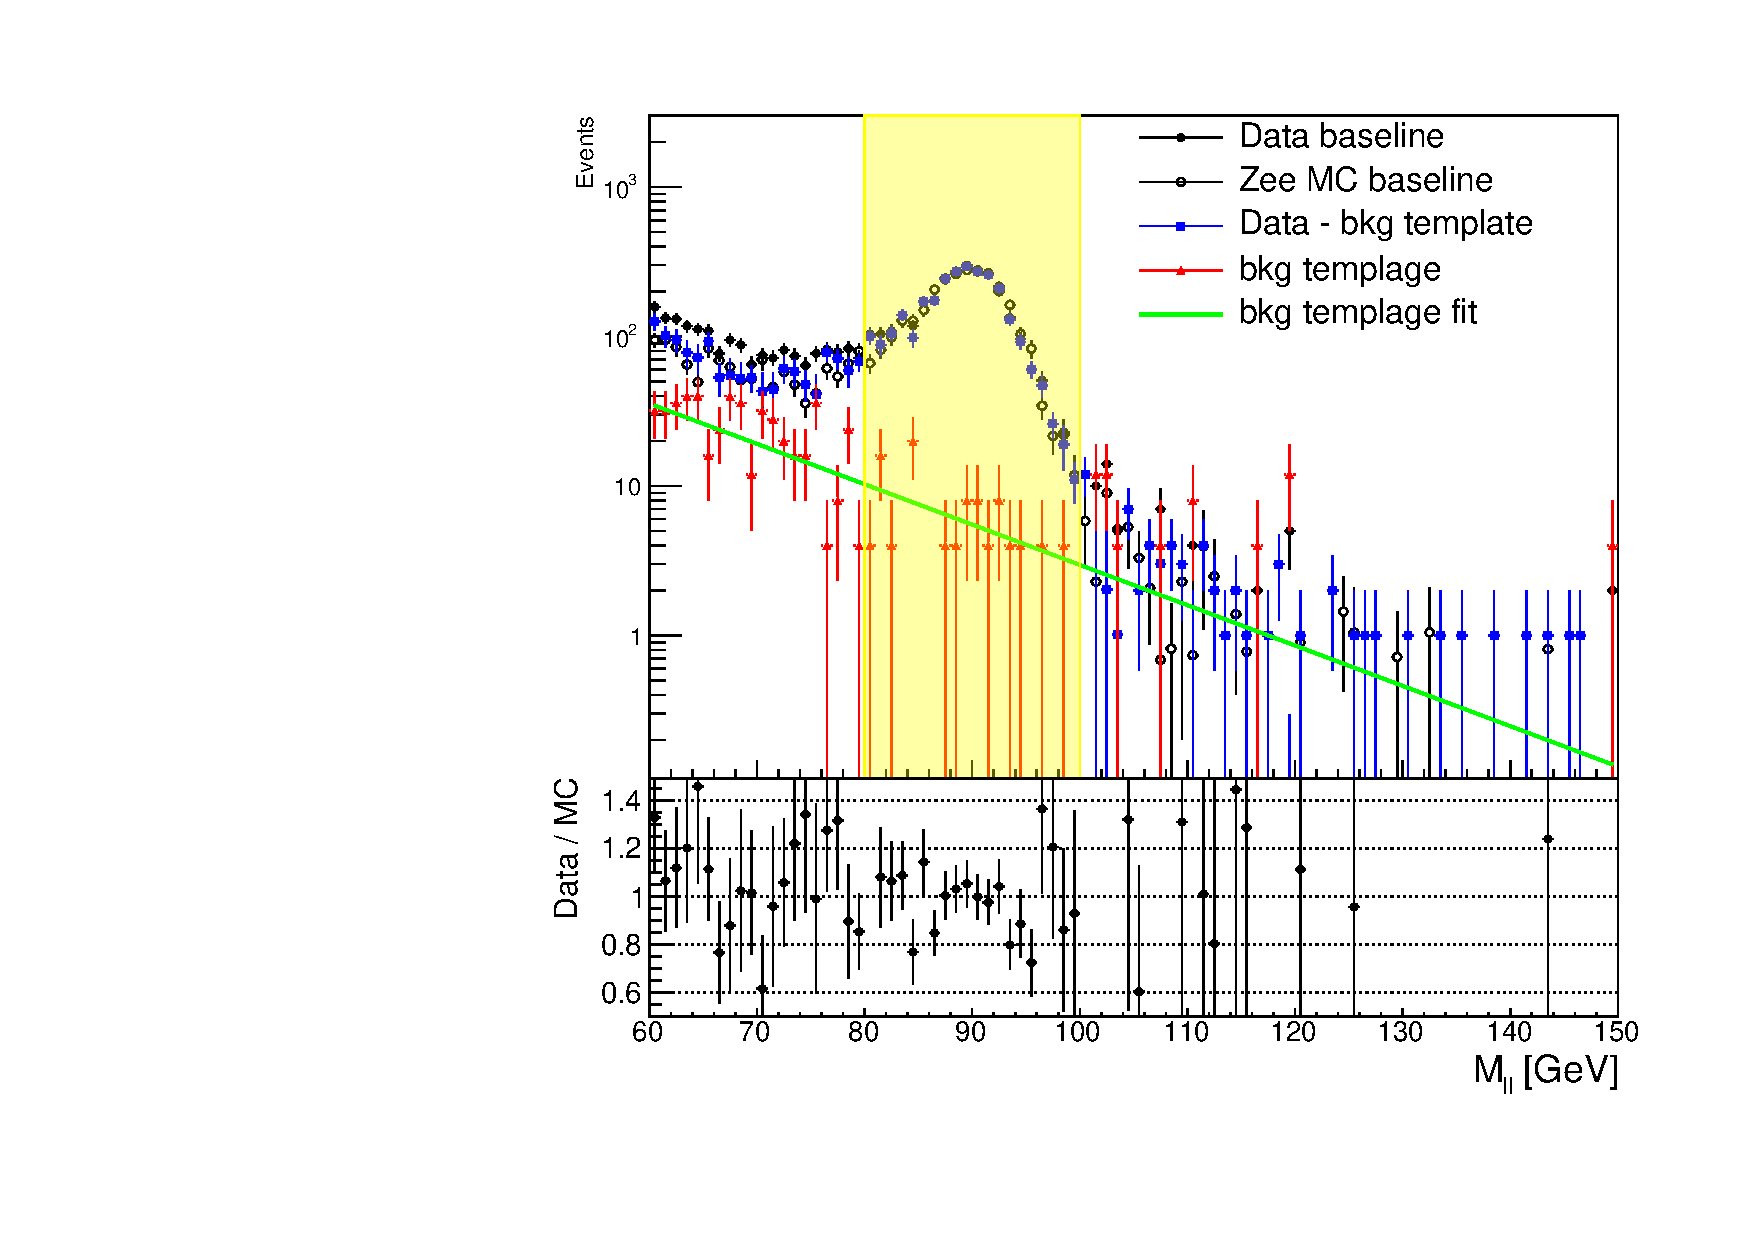
\includegraphics[scale=0.25]{bkg_subtraction_baseline_template_range_baseline_mll80_100_pt10_15_eta0_80_tag_trigger_matched.pdf}
            \caption{$10 < \pt < 15$~{\GeV}\\$0 < |\eta| < 0.8$}
        \end{center}
    \end{subfigure}
    \begin{subfigure}[b]{0.32\textwidth}
        \begin{center}
            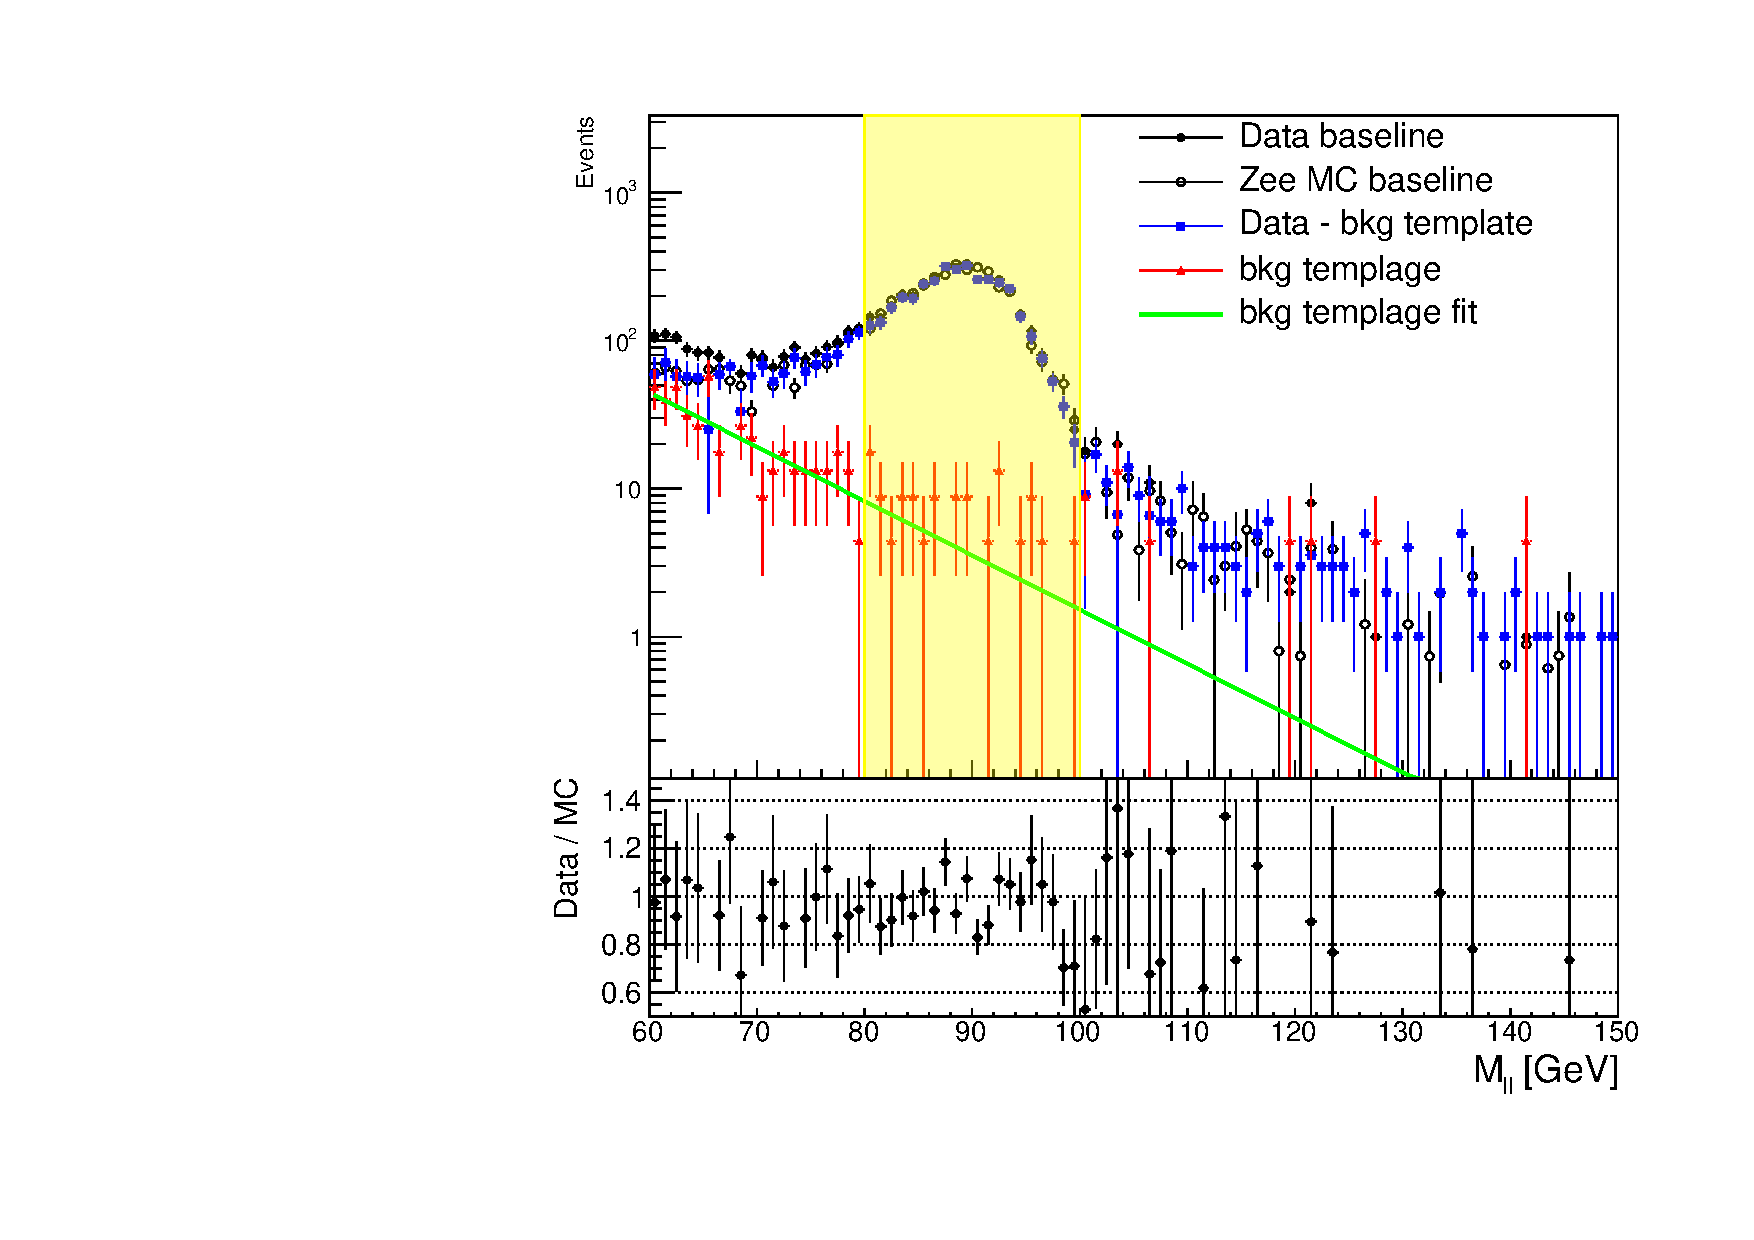
\includegraphics[scale=0.25]{bkg_subtraction_baseline_template_range_baseline_mll80_100_pt10_15_eta80_137_tag_trigger_matched.pdf}
            \caption{$10 < \pt < 15$~{\GeV}\\$0.8 < |\eta| < 1.37$}
        \end{center}
    \end{subfigure}
    \begin{subfigure}[b]{0.32\textwidth}
        \begin{center}
            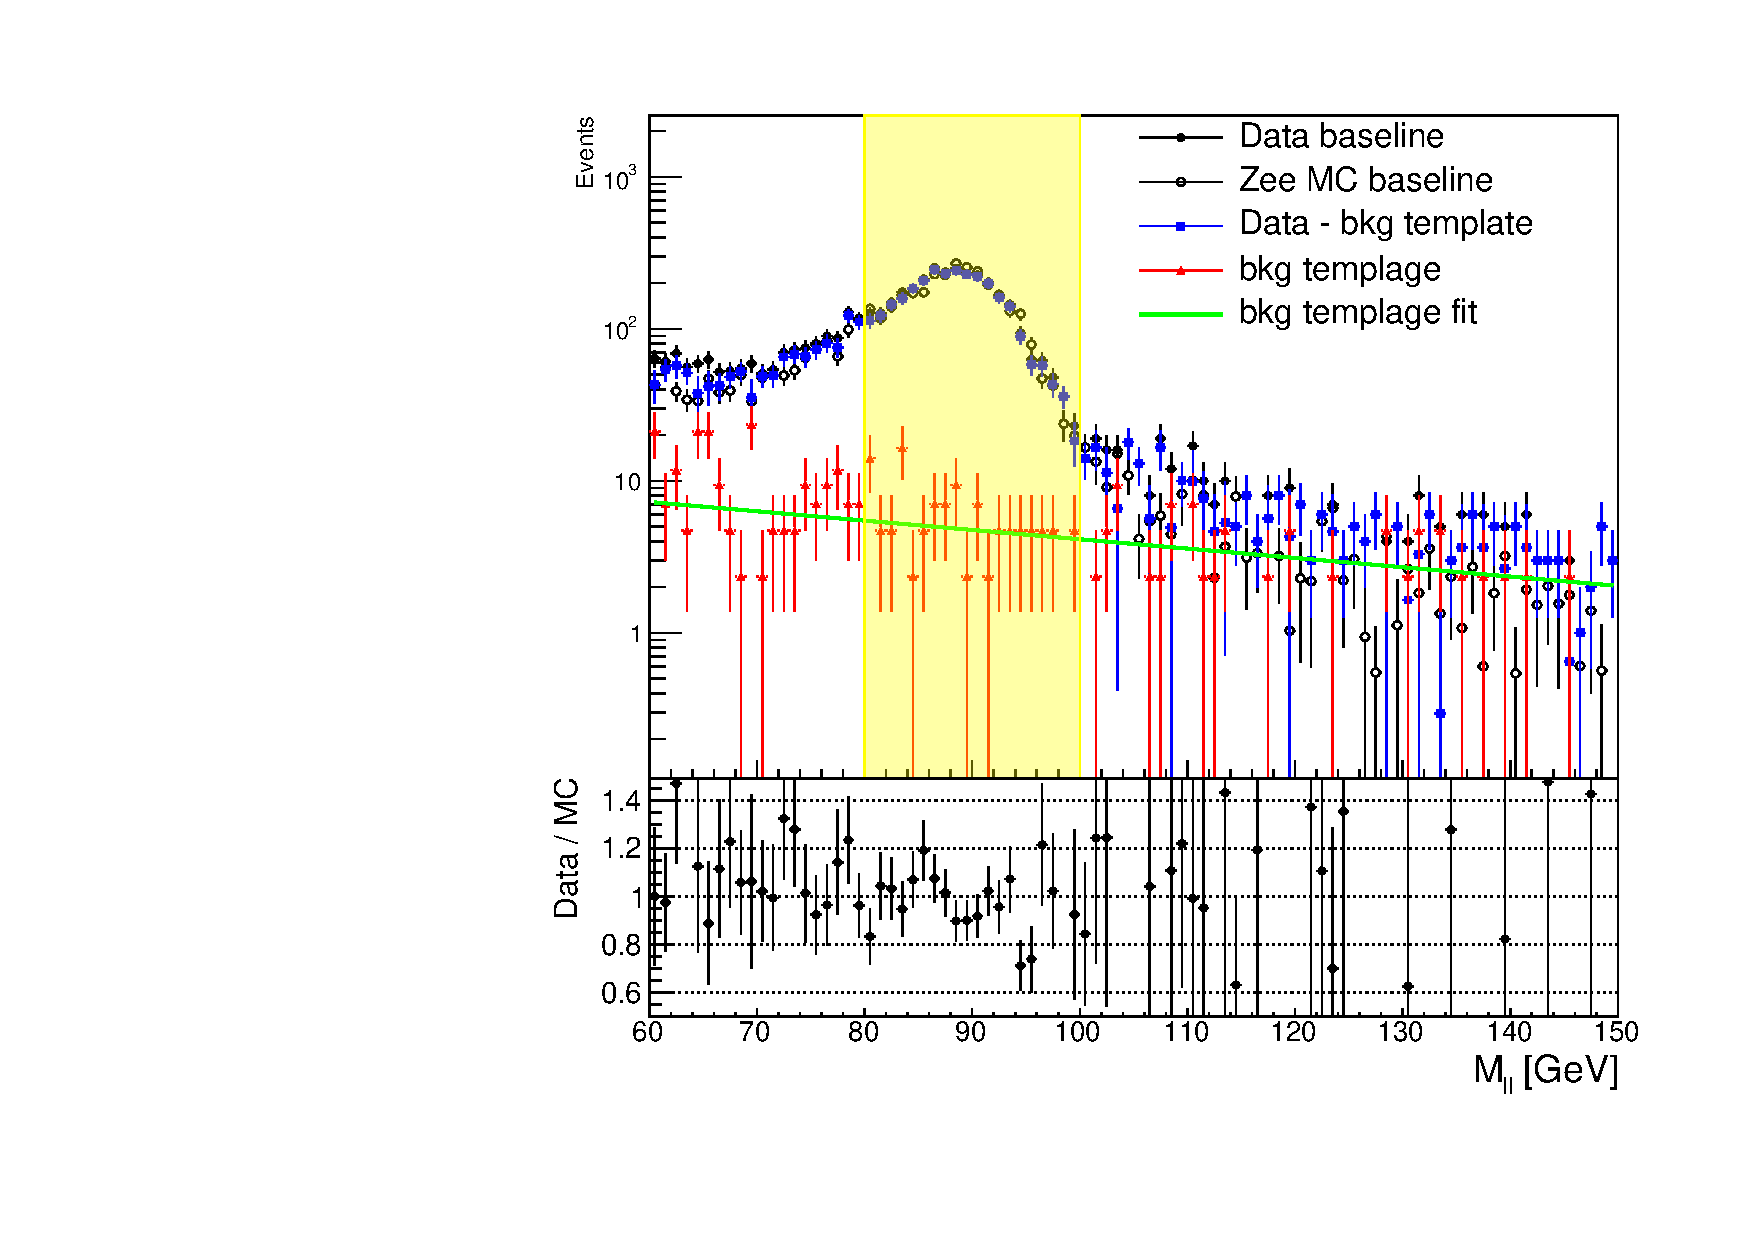
\includegraphics[scale=0.25]{bkg_subtraction_baseline_template_range_baseline_mll80_100_pt10_15_eta151_200_tag_trigger_matched.pdf}
            \caption{$10 < \pt < 15$~{\GeV}\\$1.52 < |\eta| < 2.0$}
        \end{center}
    \end{subfigure}
    \\
    \begin{subfigure}[b]{0.32\textwidth}
        \begin{center}
            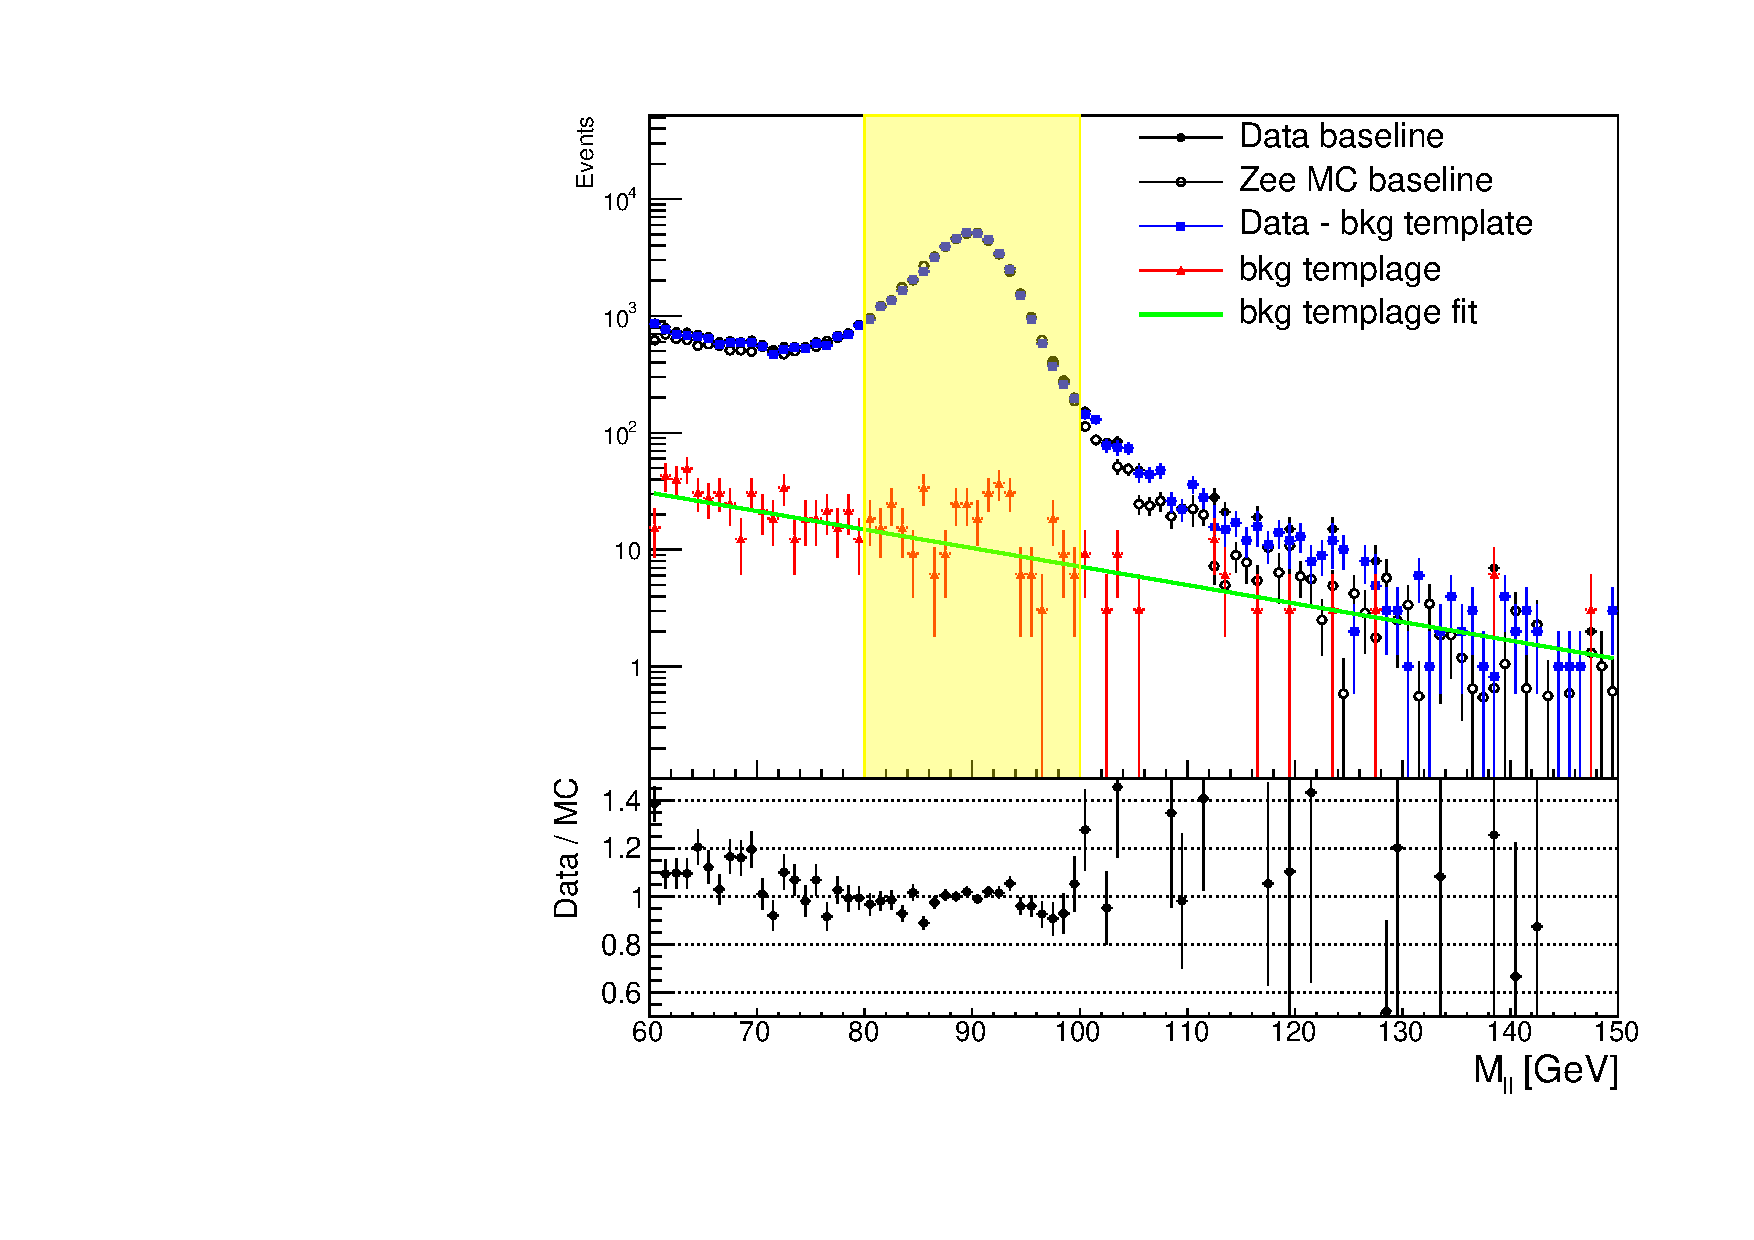
\includegraphics[scale=0.25]{bkg_subtraction_baseline_template_range_baseline_mll80_100_pt15_20_eta0_80_tag_trigger_matched.pdf}
            \caption{$15 < \pt < 20$~{\GeV}\\$0 < |\eta| < 0.8$}
        \end{center}
    \end{subfigure}
    \begin{subfigure}[b]{0.32\textwidth}
        \begin{center}
            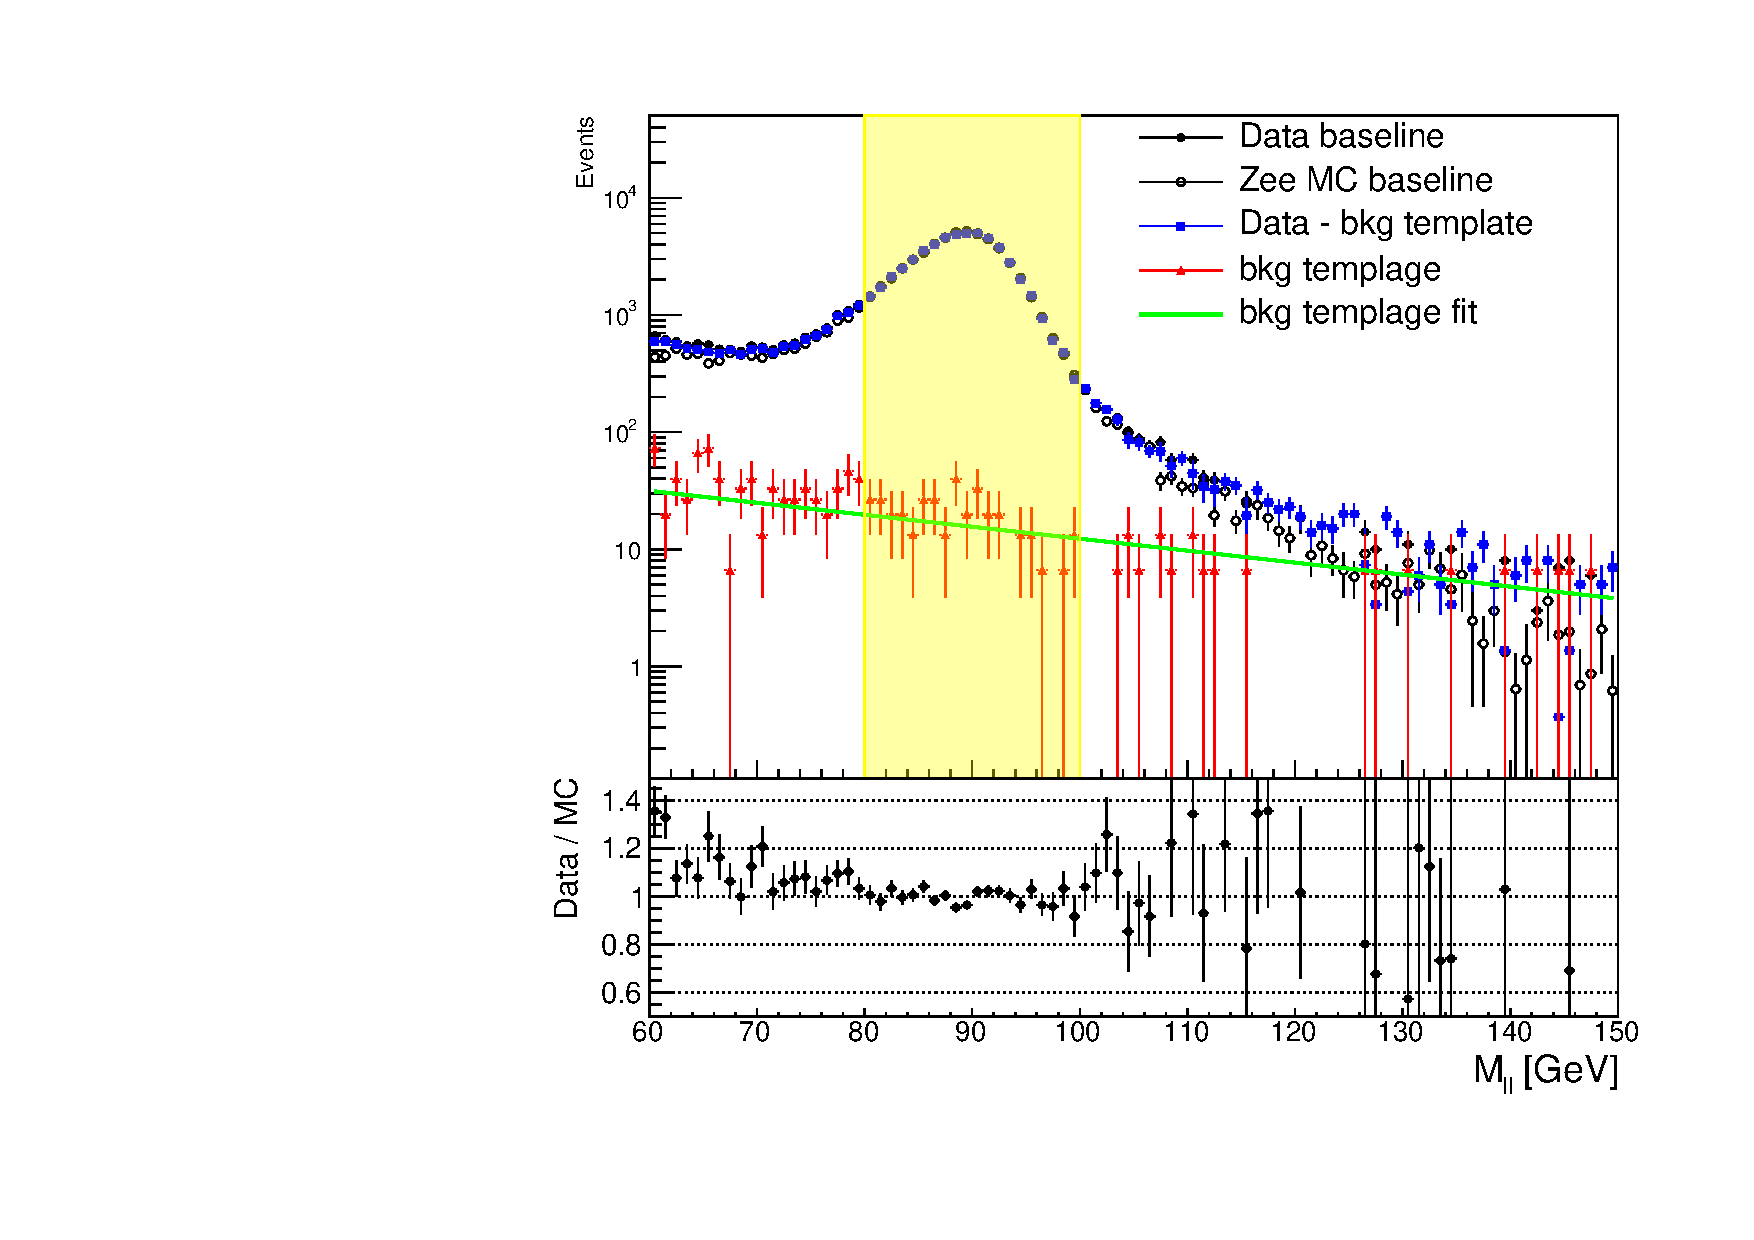
\includegraphics[scale=0.25]{bkg_subtraction_baseline_template_range_baseline_mll80_100_pt15_20_eta80_137_tag_trigger_matched.pdf}
            \caption{$15 < \pt < 20$~{\GeV}\\$0.8 < |\eta| < 1.37$}
        \end{center}
    \end{subfigure}
    \begin{subfigure}[b]{0.32\textwidth}
        \begin{center}
            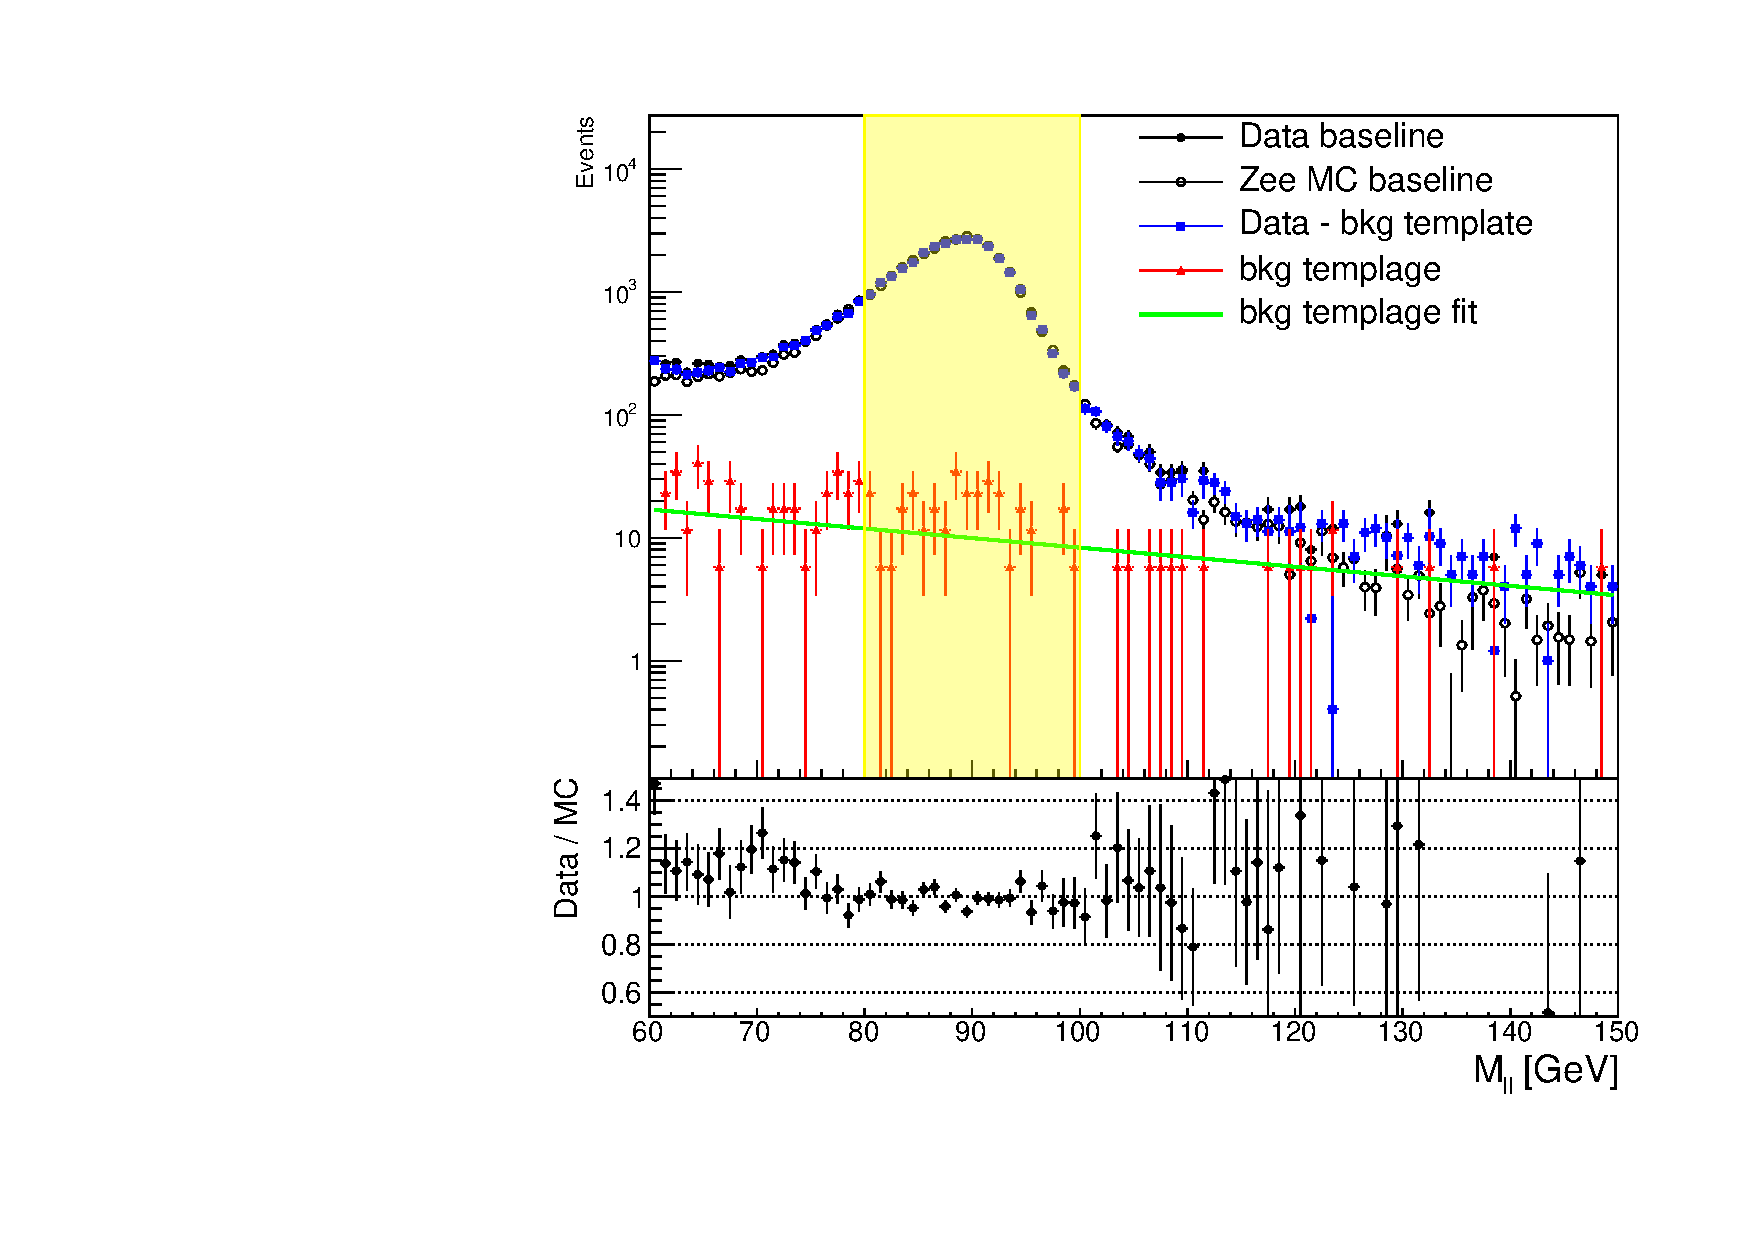
\includegraphics[scale=0.25]{bkg_subtraction_baseline_template_range_baseline_mll80_100_pt15_20_eta151_200_tag_trigger_matched.pdf}
            \caption{$15 < \pt < 20$~{\GeV}\\$1.52<|\eta|<2.0$}
        \end{center}
    \end{subfigure}
    \caption{Illustration of the background subtraction procedure.
    The full black dots and blue squares are the $m_{ee}$ distributions for data before and after performing the background subtraction, respectively.
    The $m_{ee}$ distribution for $Z \to ee$ MC, which is labeled by the open black circles, is normalized to the data after the background subtraction using a Gaussian fit of $85 < m_{ee} < 95$~{\GeV}.
    The lower panels show the data-to-MC ratio where the background subtraction has been applied on data.
    The background templates and their respective fitting results are indicated by the red triangles and green lines, respectively.
    }
    \label{fig:app_RLE_bkg_estimations}
\end{figure}

The data after performing the background subtraction, the MC simulation samples, the background template distributions, and the fitting results are also shown.
The simulated $m_{ee}$ distribution of $Z \to ee$ MC are normalized to the data, which background subtraction has been performed, using a Gaussian fit in $Z$ peak region $85 < m_{ee} < 95$~{\GeV}.
After performing the background subtraction, the data and MC have good agreement within the statistical uncertainties.

Then, the background contamination in the $Z$ mass region $80 < m_{ee} < 100$~{\GeV} is calculated using
%
\begin{equation}
    N_{bkg}^{80 < m_{ee} < 100~{\GeV}} = \int_{80}^{100} N_\mathrm{template} \ dm_{ee} \cdot \frac{N_{bkg}^\mathrm{tail}}{N_\mathrm{template}^\mathrm{tail}}
    \label{eq:RLE_bkg_in_80_mll_100}
\end{equation}
%
Table~\ref{tab:app_RLE_bkg_estimations} summarize the background estimations in different \pt and $|\eta|$ regions.

\begin{table}[htbp]
    \begin{center}
        \begin{tabular}{lccc}
            \hline
            \hline
                                  & $0 < |\eta| < 0.8$ & $0.8 < |\eta| < 1.37$ & $1.52 < |\eta| < 2.0$\\
            \hline
            $10< \pt < 15$~{\GeV} & 4.04\%             & 2.10\%                & 3.17\%\\
            $15< \pt < 20$~{\GeV} & 0.44\%             & 0.58\%                & 0.76\%\\
            \hline
            \hline
        \end{tabular}
    \end{center}
    \caption{The estimated background contamination in in different \pt and $|\eta|$ regions.
    The \pt and $|\eta|$ binnings correspond to the one used for the final measurements.}
    \label{tab:app_RLE_bkg_estimations}
\end{table}

The largest improvements are observed in the lowest \pt bin ($10 < \pt < 15$~{\GeV}) where a sizable background contamination is subtracted.
The background contamination is relatively small in the second lowest \pt bin ($15 < \pt < 20$~{\GeV}) providing the evidence that high purity of prompt leptons can be obtained using $Z$ tag-and-probe method.
Table~\ref{tab:app_RLE_efficiency_before_and_after_background_subtraction} shows the real electron efficiencies before and after performing the background subtraction.

\begin{table}[htbp]
    %\begin{center}
    \resizebox{\textwidth}{!}{% <------ Don't forget this %
        % {\footnotesize
            \begin{tabular}{lcccc}
                \hline
                \hline
                                                        & background subtraction & $0 < |\eta| < 0.8$ & $0.8 < |\eta| < 1.37$ & $1.52 <| \eta| < 2.0$\\
                \hline
                \multirow{2}{*}{$10 < \pt < 15$~{\GeV}} & before                 & $57.4 \pm 0.9$     & $66.6 \pm 0.8$        & $53.2 \pm 0.9$\\
                                                        & after                  & $59.9 \pm 1.9$     & $68.0 \pm 1.8$        & $55.0 \pm 1.7$\\
                \hline
                \multirow{2}{*}{$15 < \pt < 20$~{\GeV}} & before                 & $64.5 \pm 0.2$     & $69.4 \pm 0.2$        & $62.0 \pm 0.3$\\
                                                        & after                  & $64.8 \pm 0.5$     & $69.8 \pm 0.5$        & $62.5 \pm 0.6$\\
                \hline
                \hline
            \end{tabular}
        % }
    }
    %\end{center}
    \caption{The real electron efficiencies before and after performing the background subtraction in different \pt and $|\eta|$ regions are shown in percentage.}
    \label{tab:app_RLE_efficiency_before_and_after_background_subtraction}
\end{table}

%%%
%%%
%%%

\section{Cut efficiencies}
\label{sec:app_RLE_cut_efficiencies}
Figure~\ref{fig:app_RLE_cut_efficiencies} shows the efficiencies associated to each signal cut with respect to baseline definitions.
The prompt electron efficiency increases with \pt from $\sim$62\% to $\sim$98\% and the efficiency losses are dominated by the calorimeter isolation.
The calorimeter isolation cut efficiency increases with \pt from $\sim$ 69\% to $\sim$98\%.
The loose to medium likelihood (LH) cut efficiency increases from $\sim$92\% to $\sim$96\% in the $10< \pt < 30$~{\GeV} then reaches a plateau when $30 < \pt < 50$~{\GeV} and increases again to $\sim$98\% when $\pt > 60$~{\GeV}.
The track isolation cut efficiency increases from $\sim$89\% at low \pt to $\sim$100\% when $\pt > 60$~{\GeV}.
The longitudinal impact parameter cut efficiency increases from $\sim$98\% at low \pt to $\sim$100\% when $\pt > 15$~{\GeV}.
The cut efficiencies for muon are much higher than the electron case because the same muon identification is used for the baseline and the signal muon definitions.
The associated efficiencies computed using $Z\to \mu \mu$ events increase from $\sim$80\% for $10 < \pt < 15$~{\GeV} to $\sim$98\% when $\pt > 50$~{\GeV}.
The dominant contribution is the track isolation cut efficiency which increases from $\sim$82\% to 98\% when $\pt > 50$~{\GeV}.
The transverse and longitudinal impact parameter cut efficiencies are $\sim$99\% and 100\%, respectively.
For the electron case, the transverse impact parameter cut is already applied at the baseline level

\begin{figure}[htbp]
    \begin{subfigure}[b]{0.48\textwidth}
        \begin{center}
            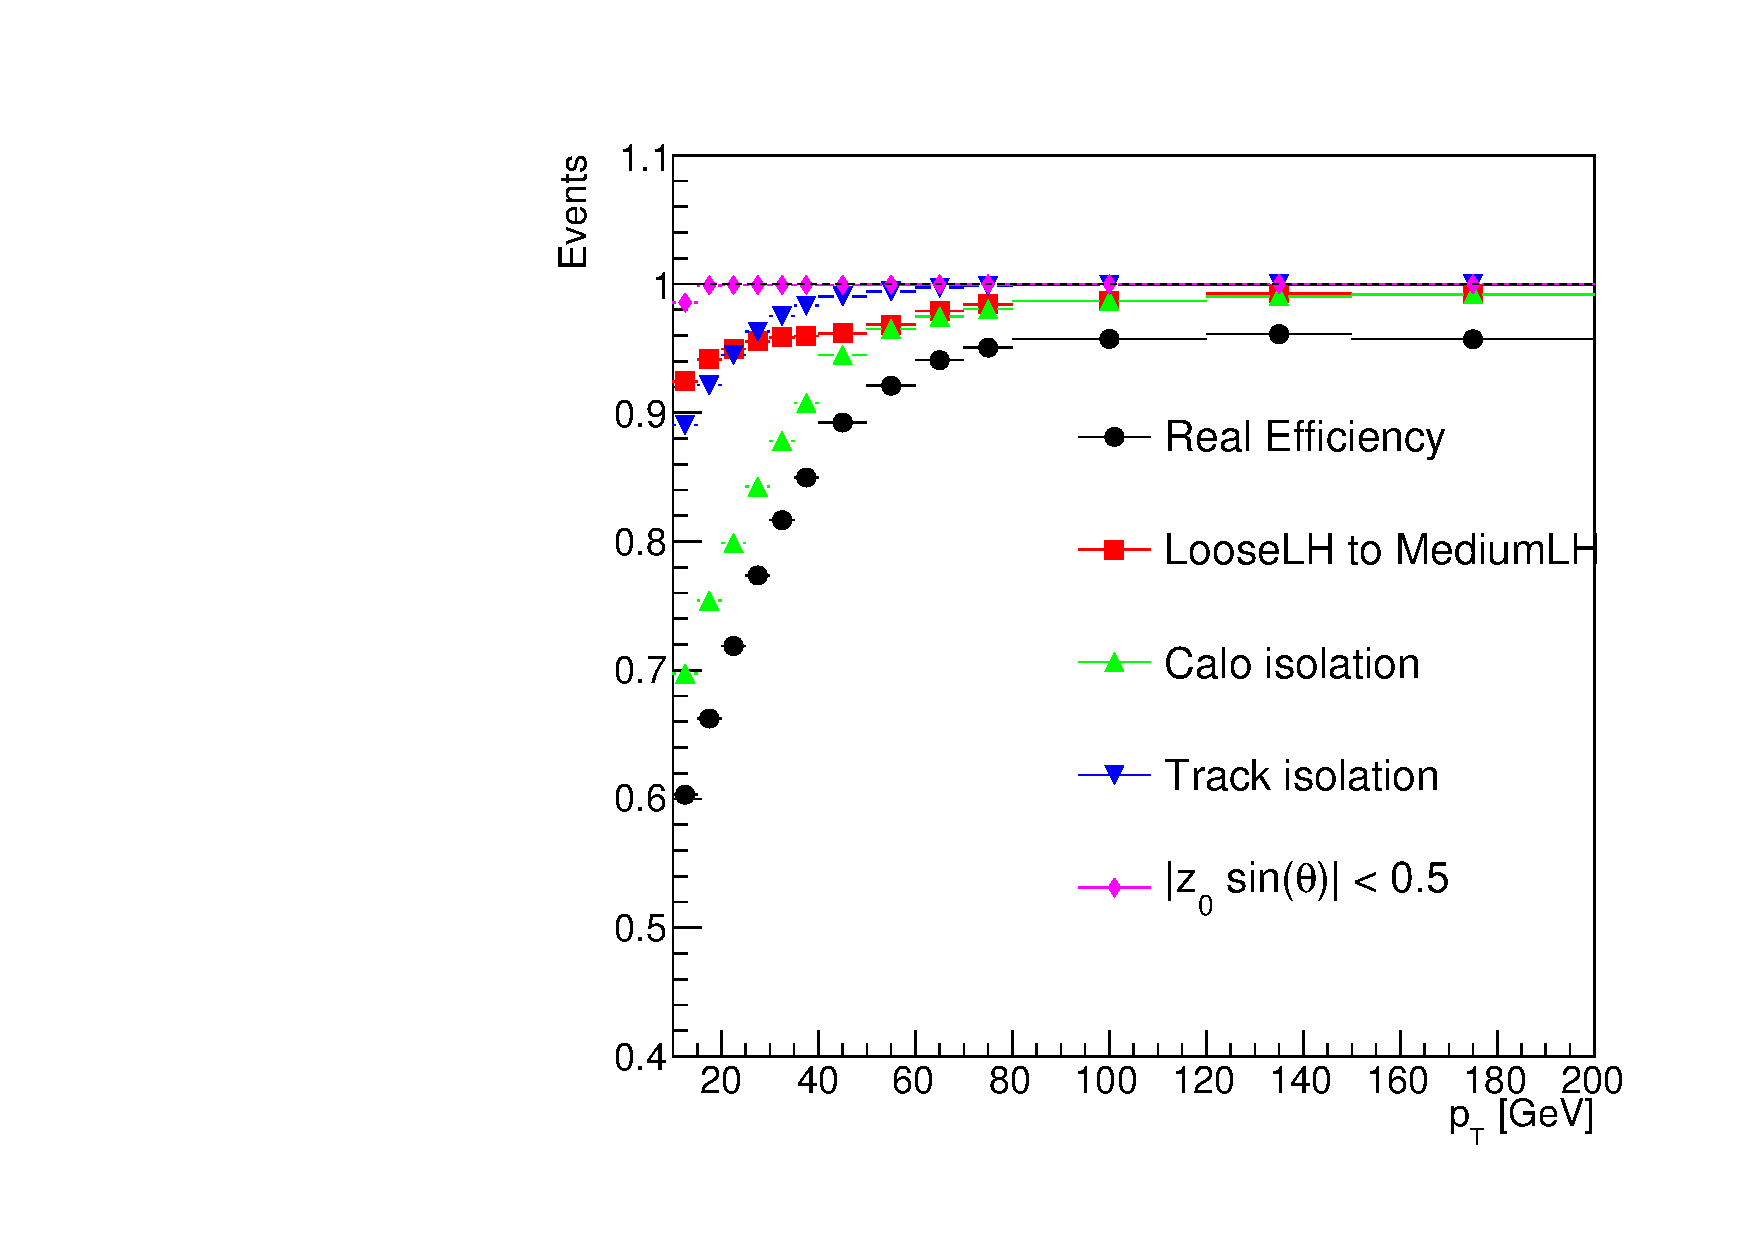
\includegraphics[scale=0.35]{cut_efficiency_electron.pdf}
            \caption{Electron}
        \end{center}
    \end{subfigure}
    \begin{subfigure}[b]{0.48\textwidth}
        \begin{center}
            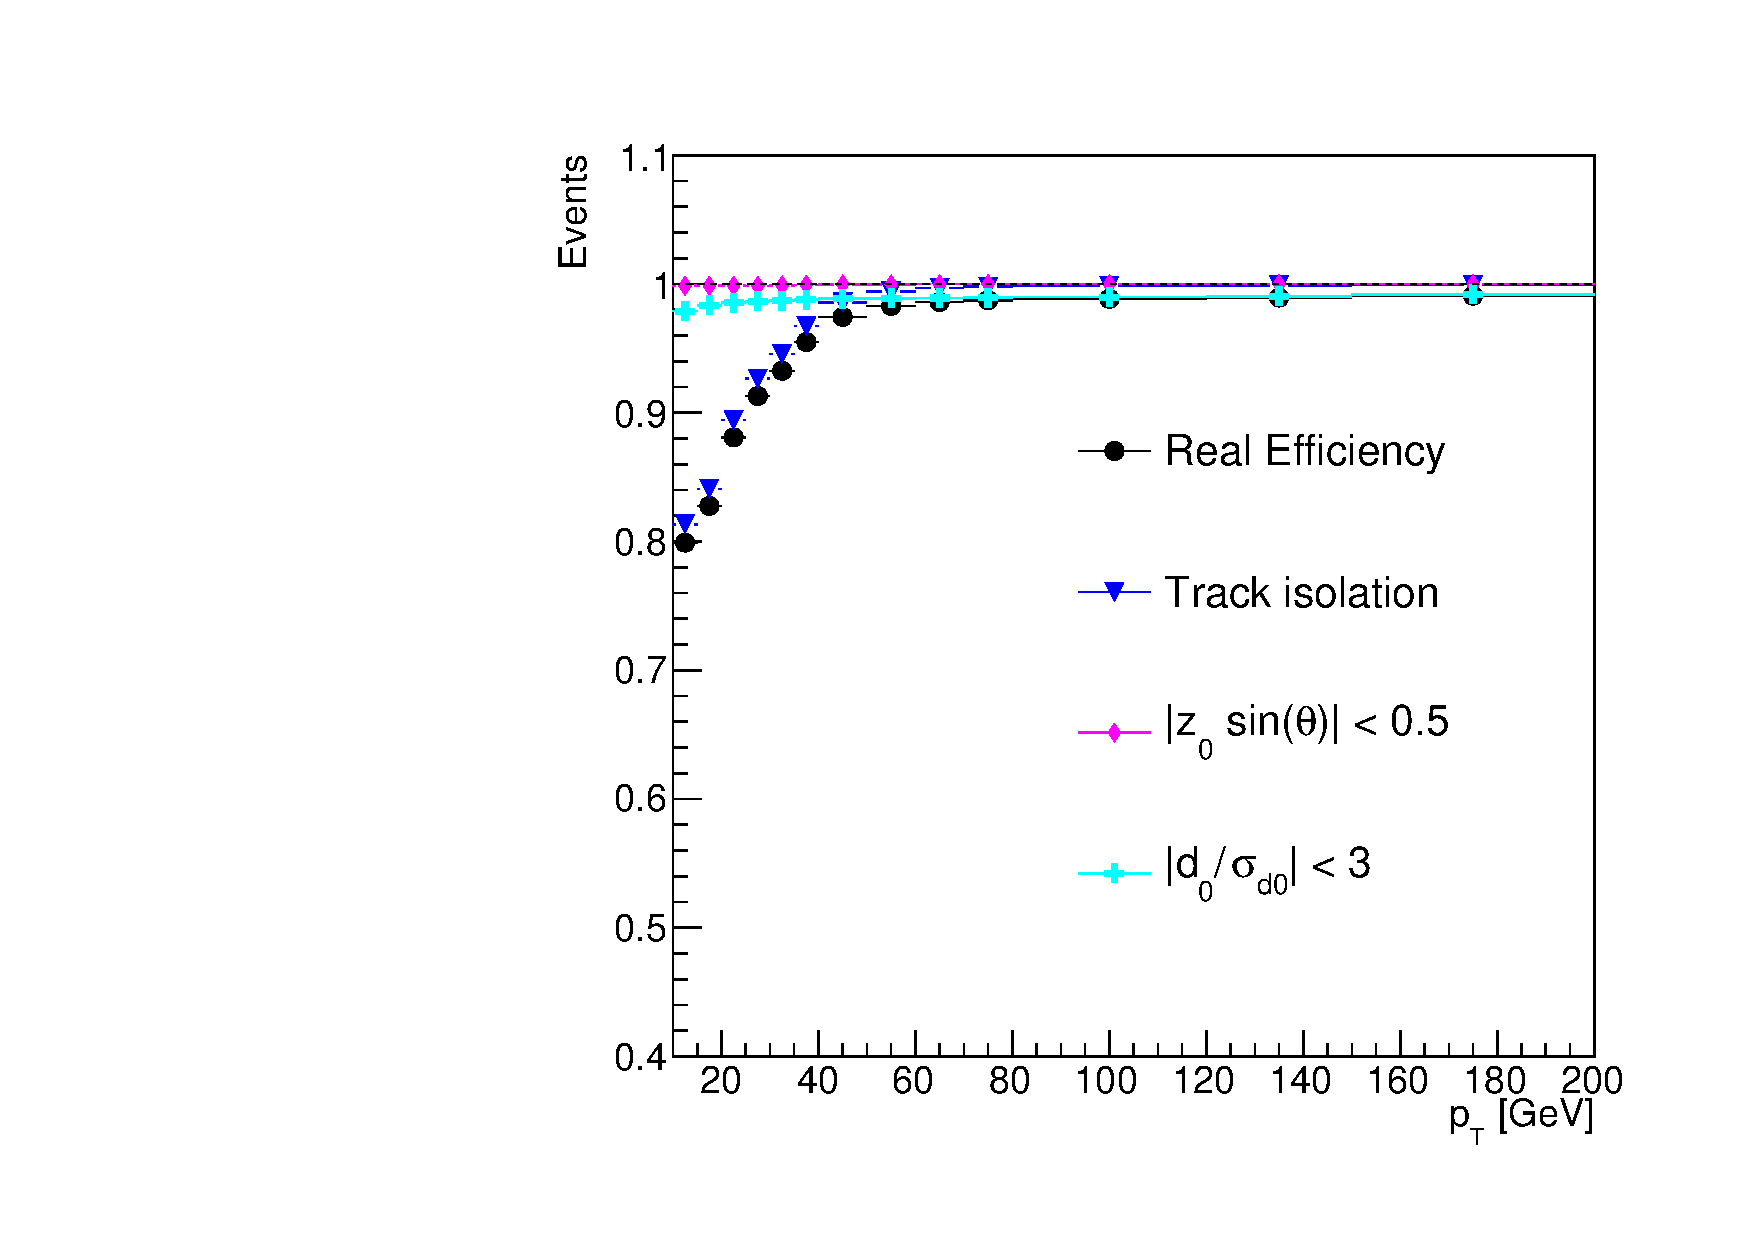
\includegraphics[scale=0.35]{cut_efficiency_muon.pdf}
            \caption{Muon}
        \end{center}
    \end{subfigure}
    \caption{Cut efficiencies of the signal electron and muon definition as a function of \pt.
    The total real electron and muon efficiencies are presented by black points. 
    The loose to medium likelihood cut efficiency is presented by red squares.
    The calorimeter and track isolation cut efficiencies are presented by green triangles and blue triangles, respectively.
    The longitudinal and transverse impact parameters cut efficiencies are presented by magenta diamonds and cyan crosses, respectively.}
    \label{fig:app_RLE_cut_efficiencies}
\end{figure}

%%%
%%%
%%%

\section{Real lepton efficiencies}
\label{sec:app_RLE}
The real lepton efficiencies as a function of \pt and $|\eta|$ are shown in Fig~\ref{fig:app_RLE_real_efficiency_total_systematics} where the background subtraction has been applied on the electron case in $10 < \pt < 15$~{\GeV} and $15 < \pt < 20$~{\GeV}.
The uncertainties are the quadratic sum of the statistical uncertainties and the measurement systematic uncertainties.
The 3 $|\eta|$ binnings for the electron case are driven by the geometry of ECAL.
The crack region, $1.37<|\eta|<1.52$, is removed from the real electron efficiency study.
It is expected that the electron efficiencies in $1.52<|\eta|<2.01$ are lower because the electron identification is better in the central region of the ECAL.

\begin{figure}[htbp]
    \begin{subfigure}[b]{0.48\textwidth}
        \begin{center}
            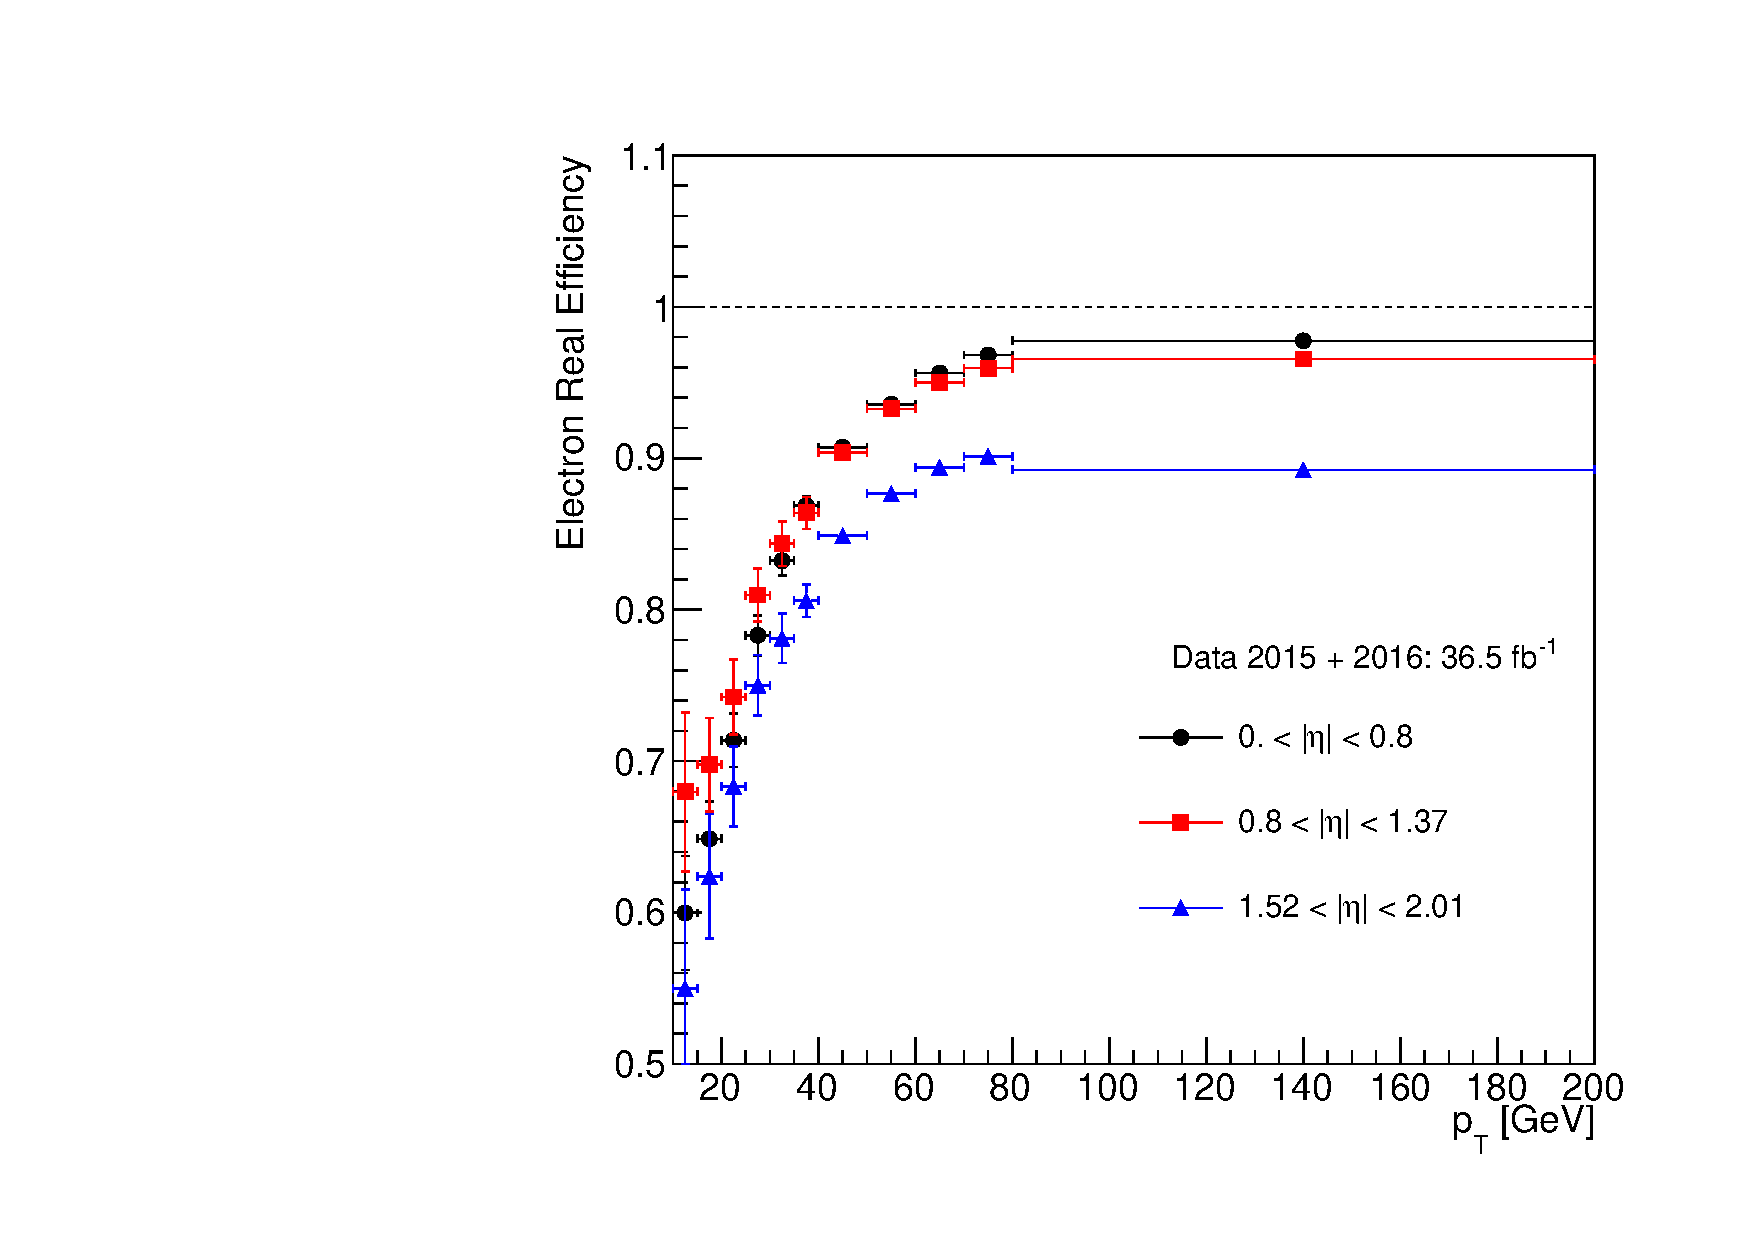
\includegraphics[scale=0.35]{real_electron_efficiency_total_systematics.pdf}
            \caption{Electron}
        \end{center}
    \end{subfigure}
    \begin{subfigure}[b]{0.48\textwidth}
        \begin{center}
            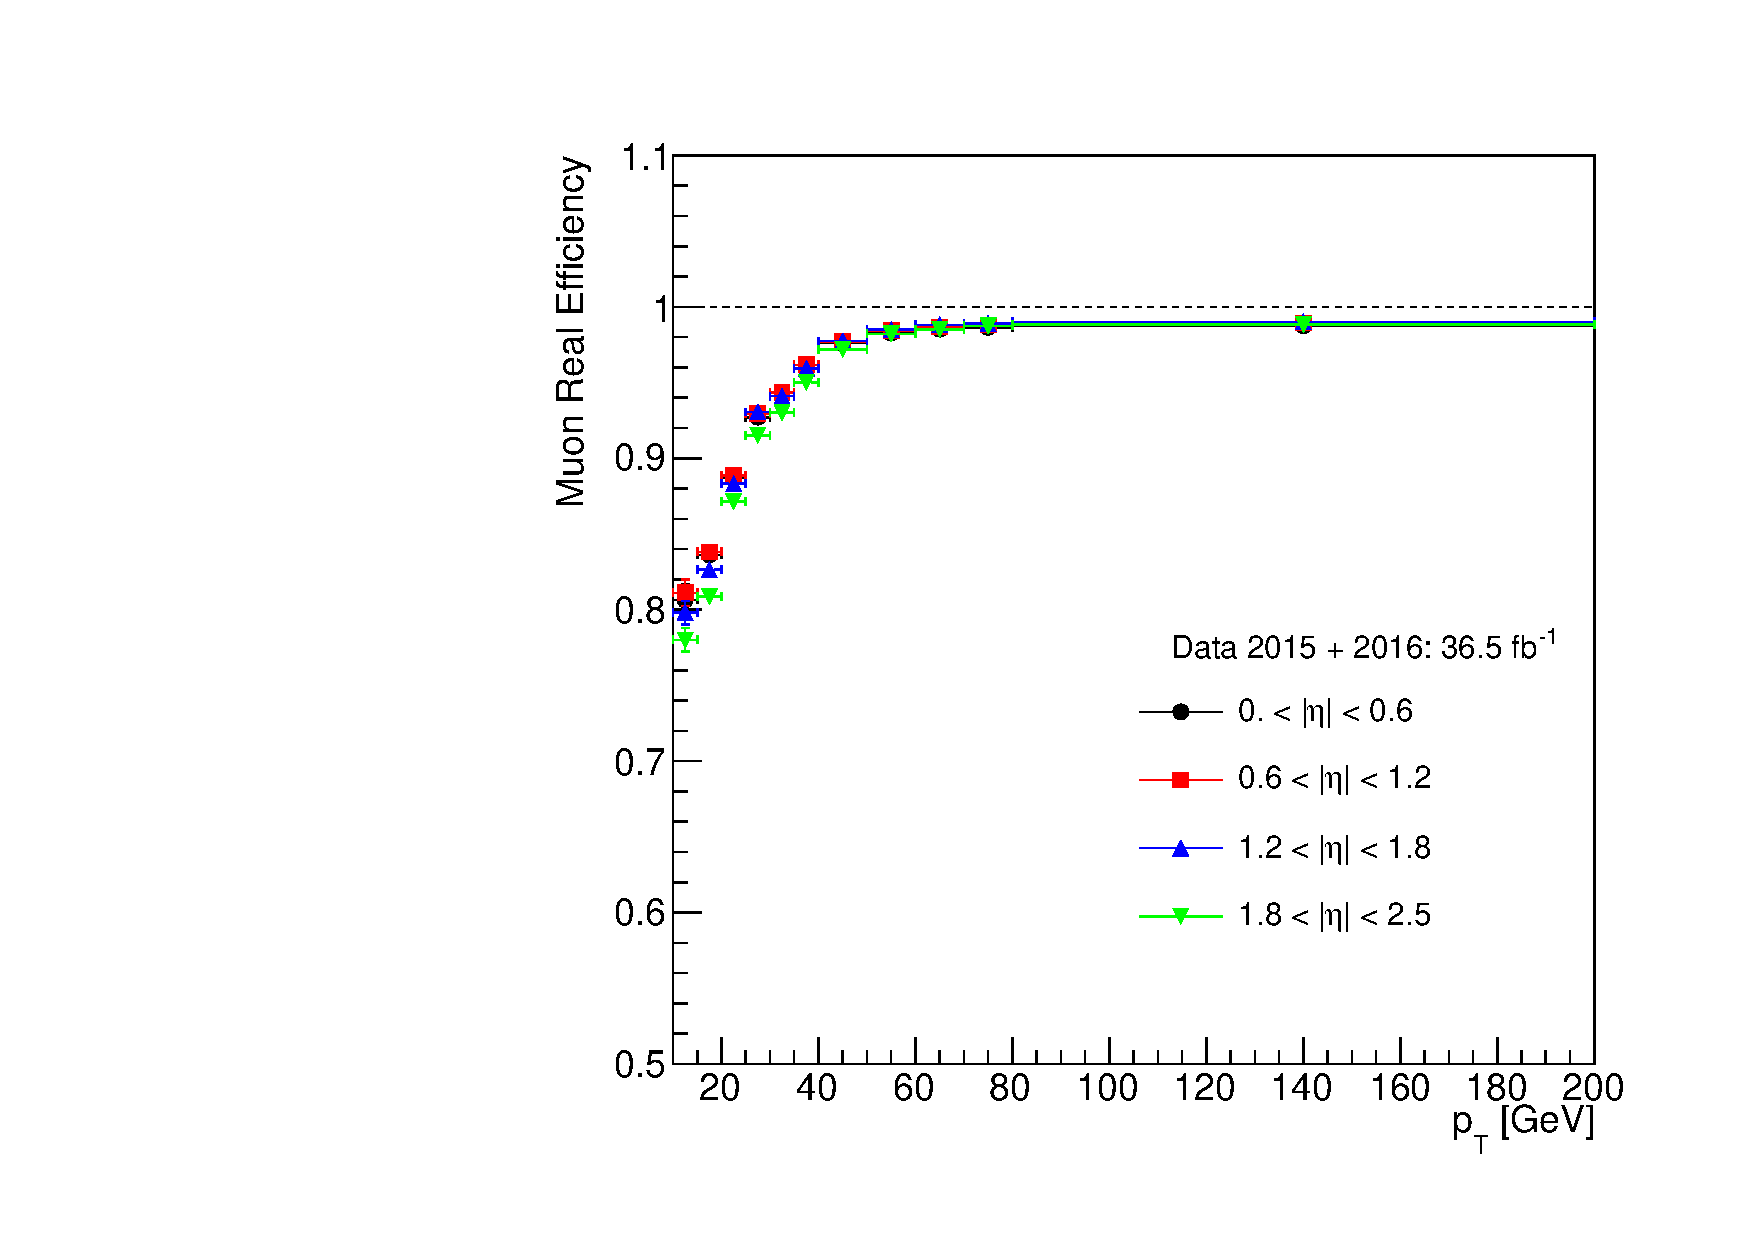
\includegraphics[scale=0.35]{real_muon_efficiency_total_systematics.pdf}
            \caption{Muon}
        \end{center}
    \end{subfigure}
    \caption{The real lepton efficiencies as a function of \pt and $|\eta|$ measured using the $Z$ tag-and-probe method.
    For the real electron efficiencies measurement, the $|\eta|$ binning in the creak region is removed.
    A homogeneous $|\eta|$ binnings are used for the muon case.}
    \label{fig:app_RLE_real_efficiency_total_systematics}
\end{figure}

%%%
%%%
%%%

\begin{figure}[htb]
    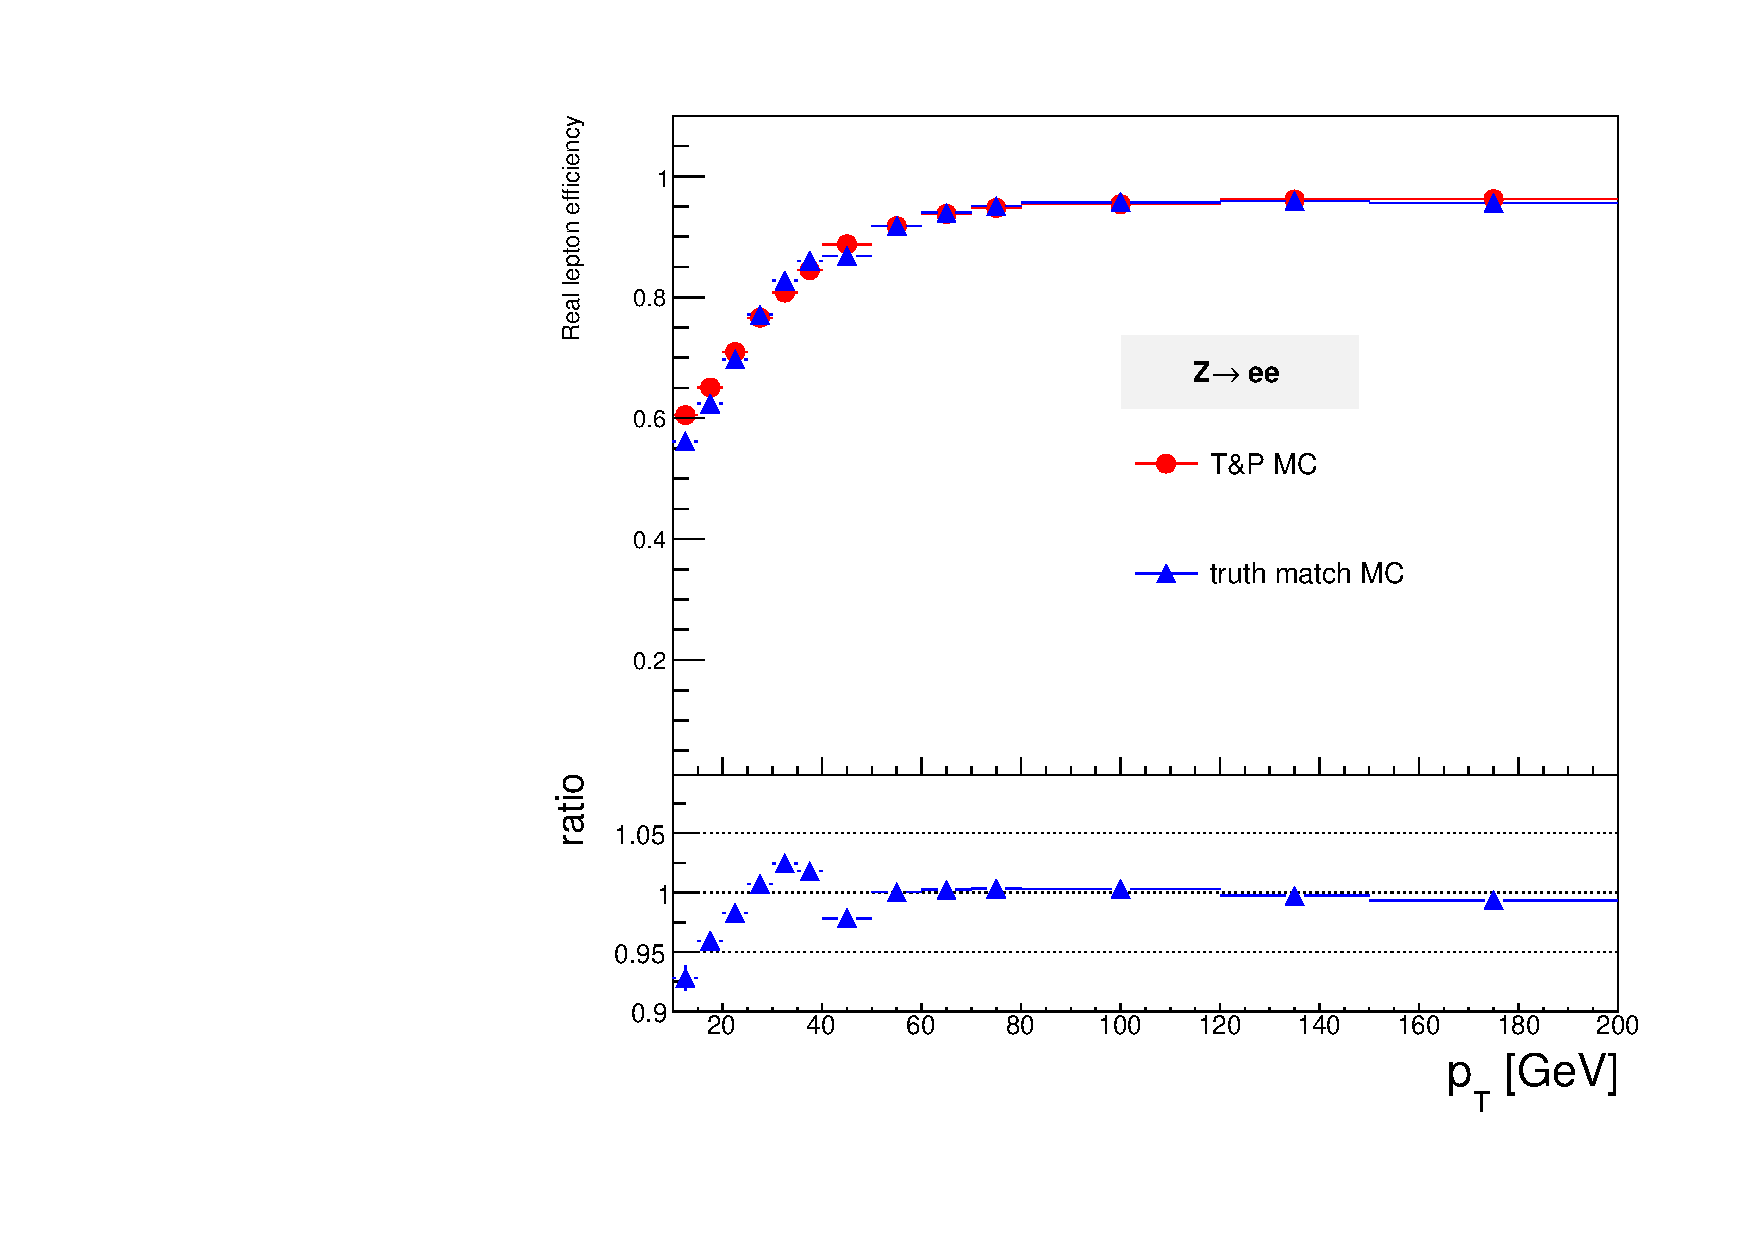
\includegraphics[width=0.32\textwidth]{Compare_TandP_truth_match_electron_pt.pdf}
    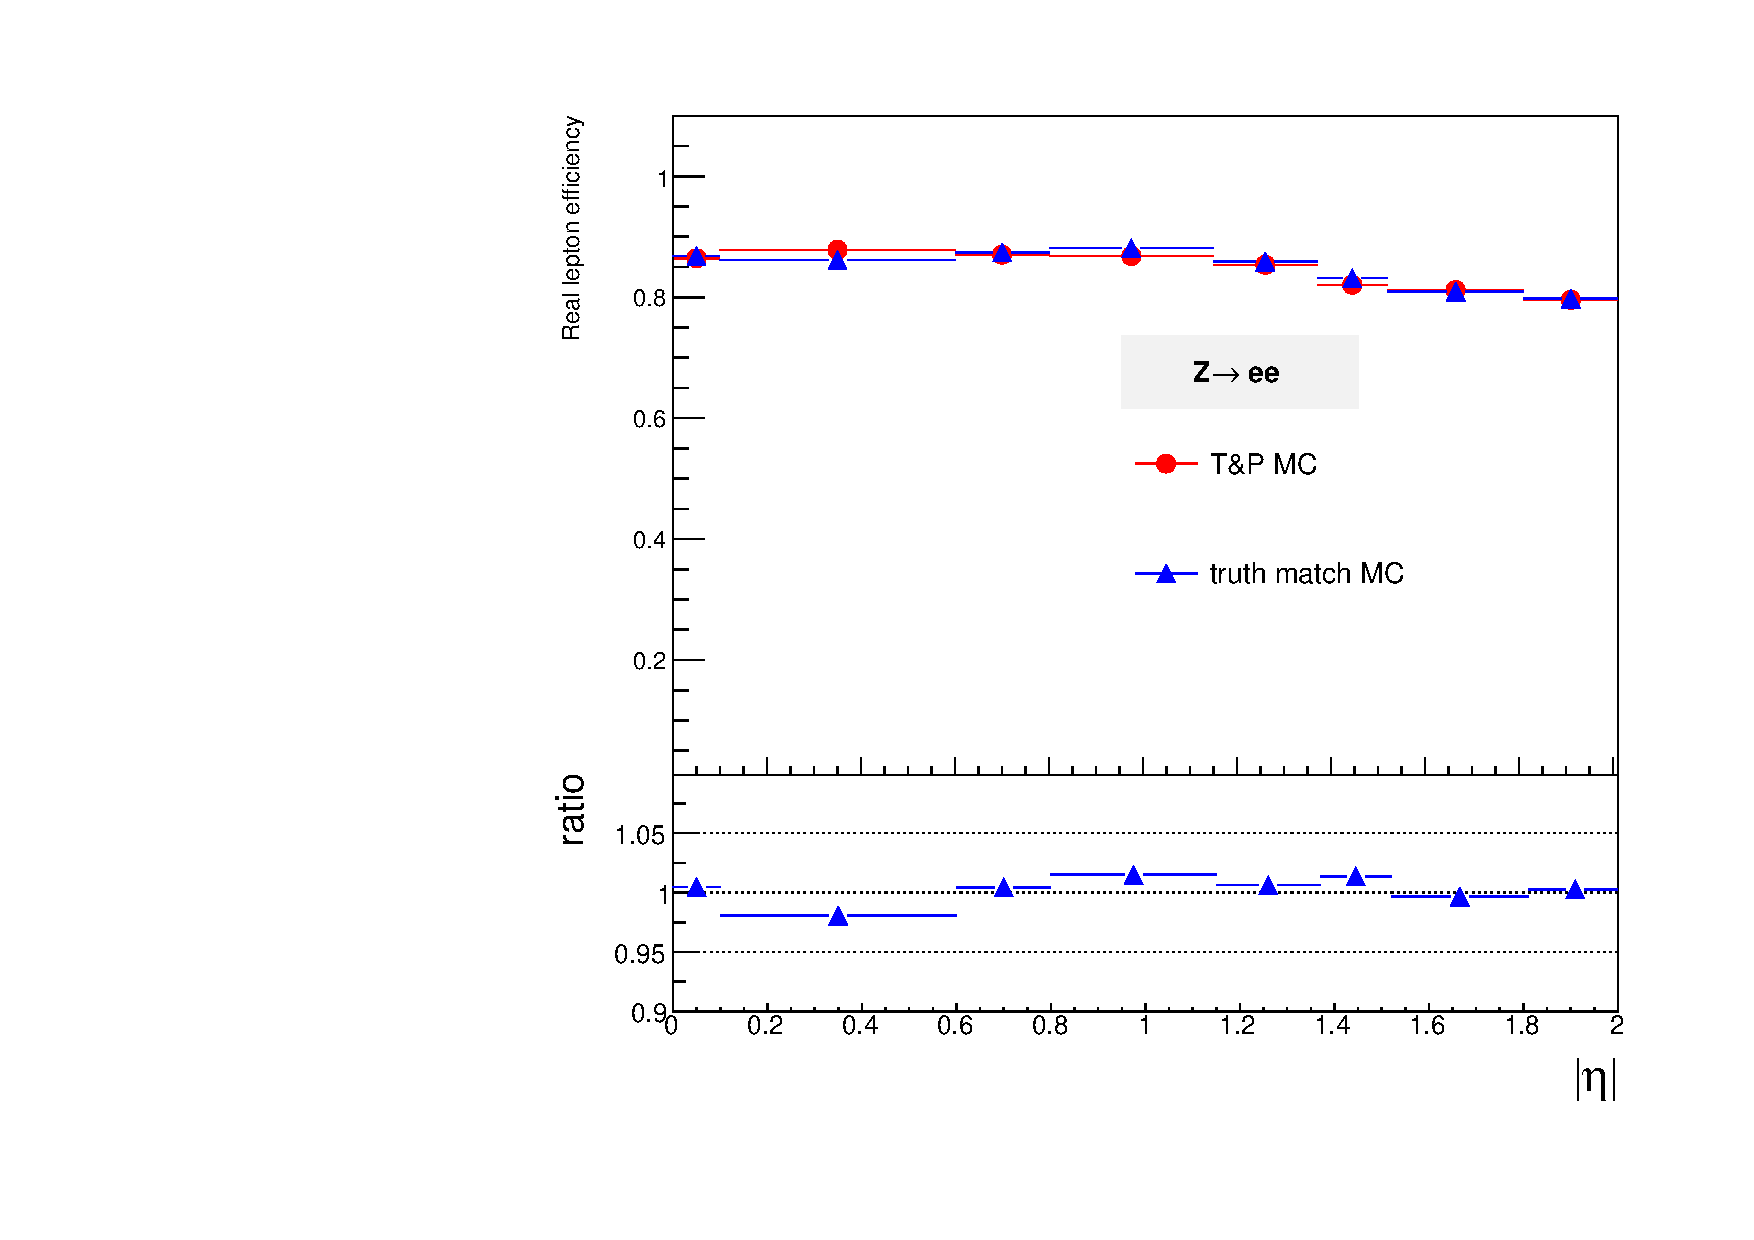
\includegraphics[width=0.32\textwidth]{Compare_TandP_truth_match_electron_eta.pdf}
    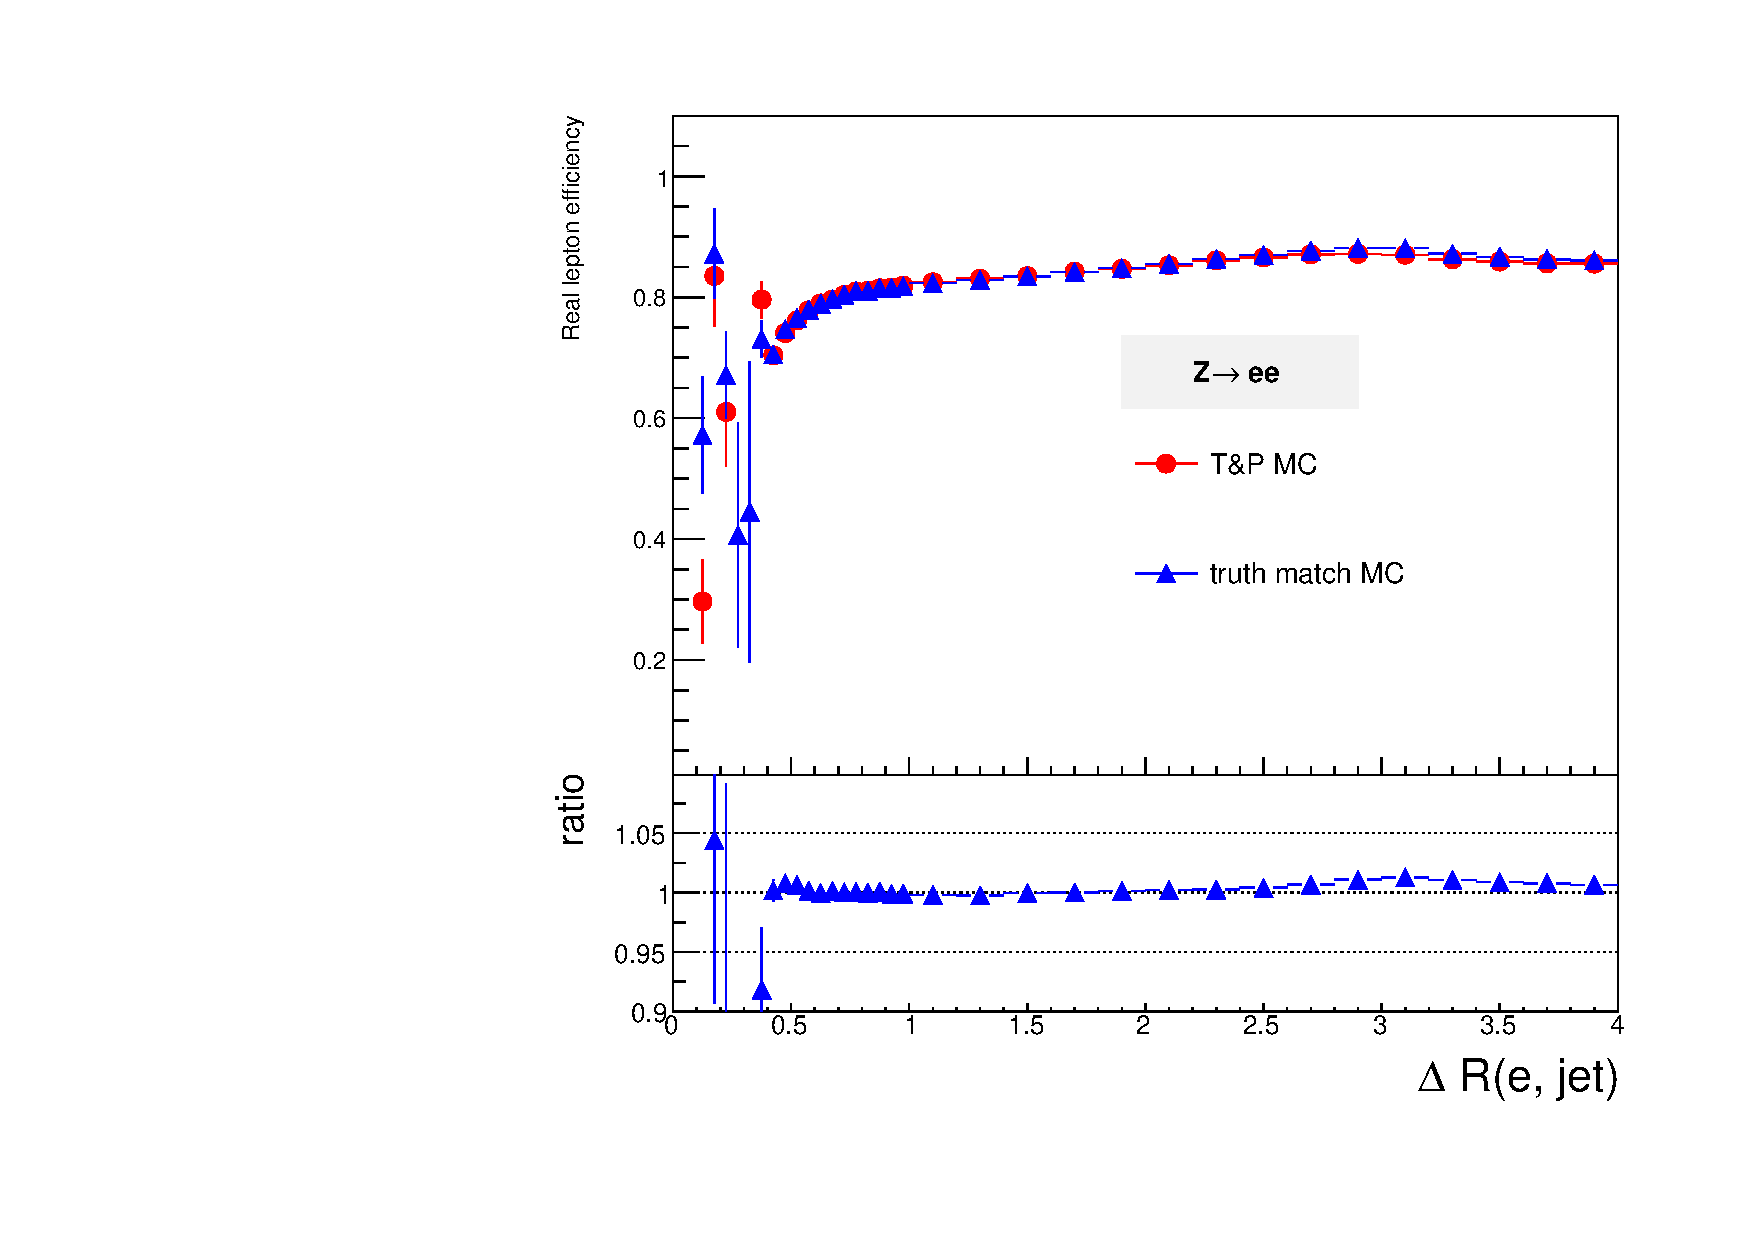
\includegraphics[width=0.32\textwidth]{Compare_TandP_truth_match_electron_dRjet.pdf}\\
    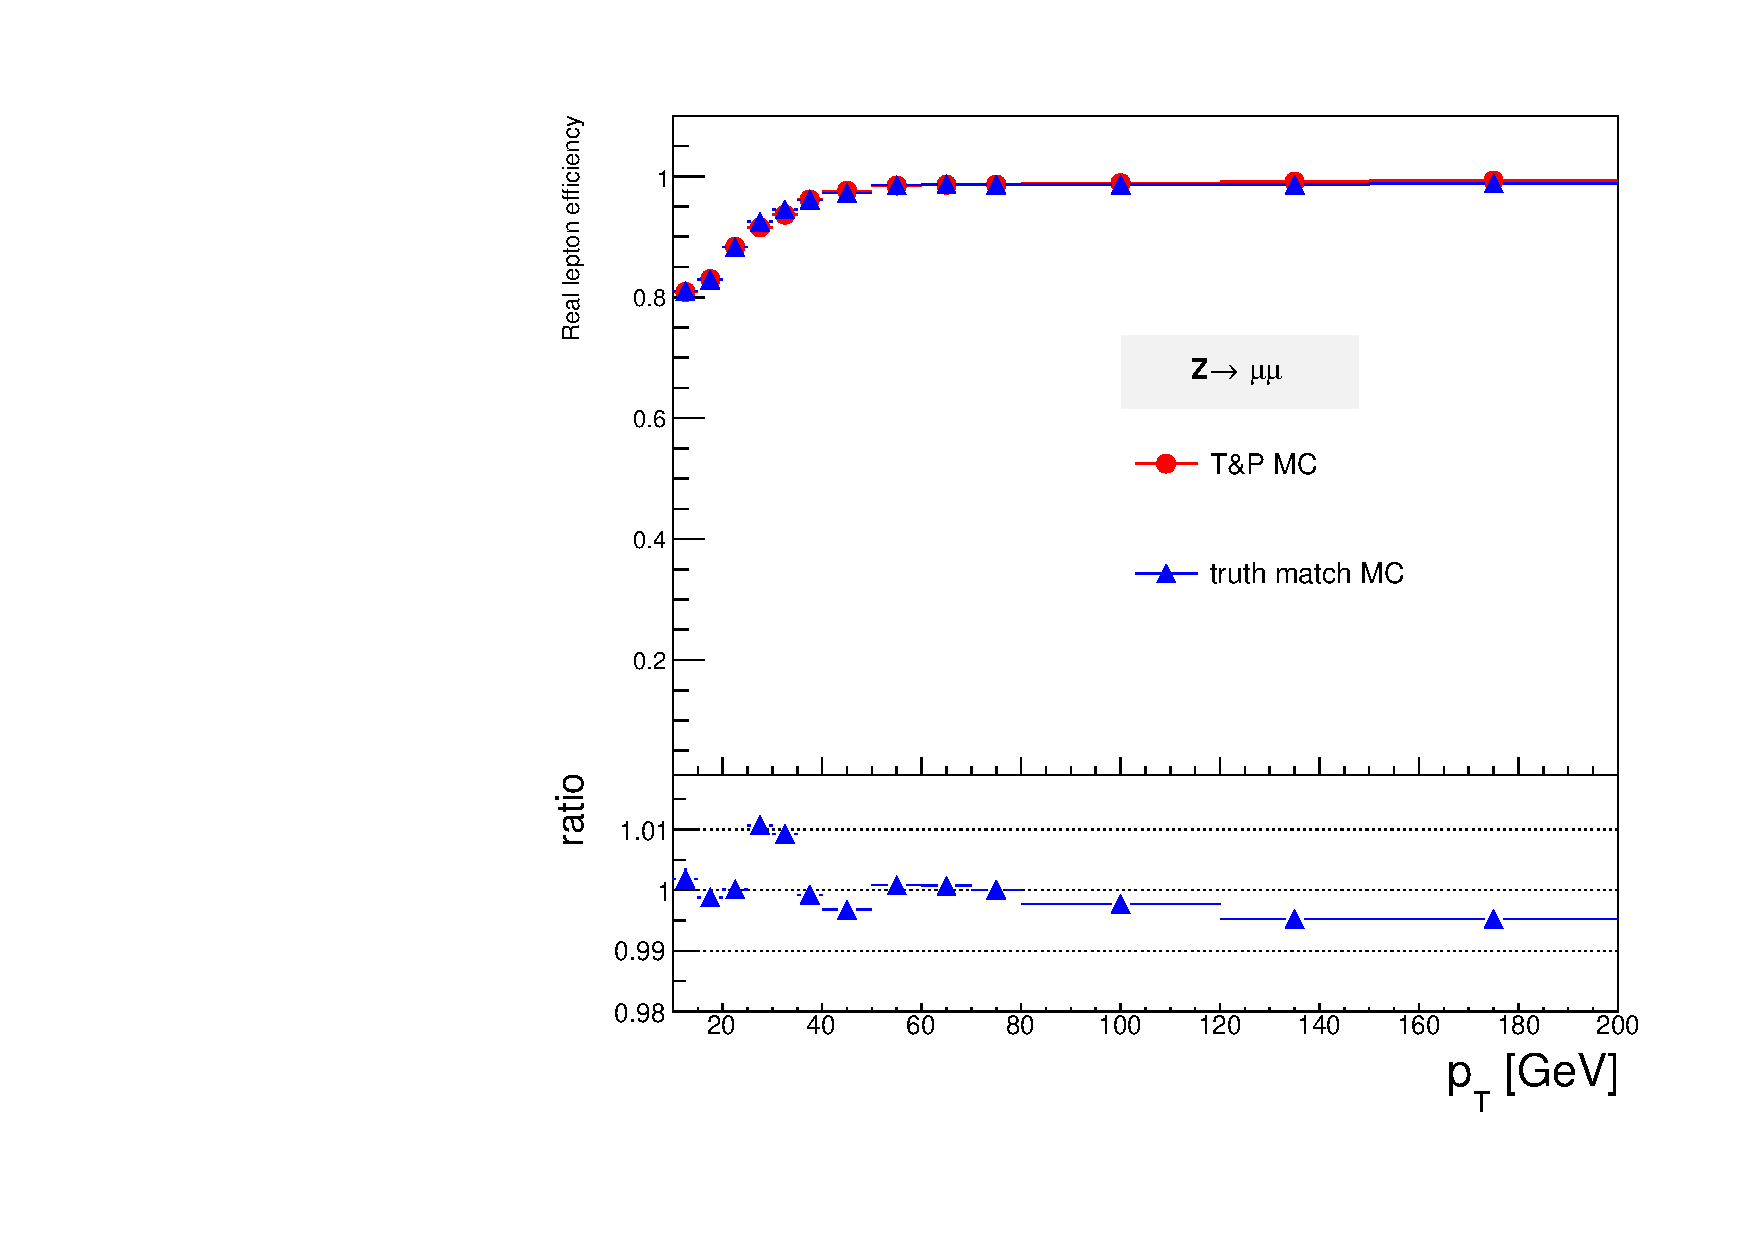
\includegraphics[width=0.32\textwidth]{Compare_TandP_truth_match_muon_pt.pdf}
    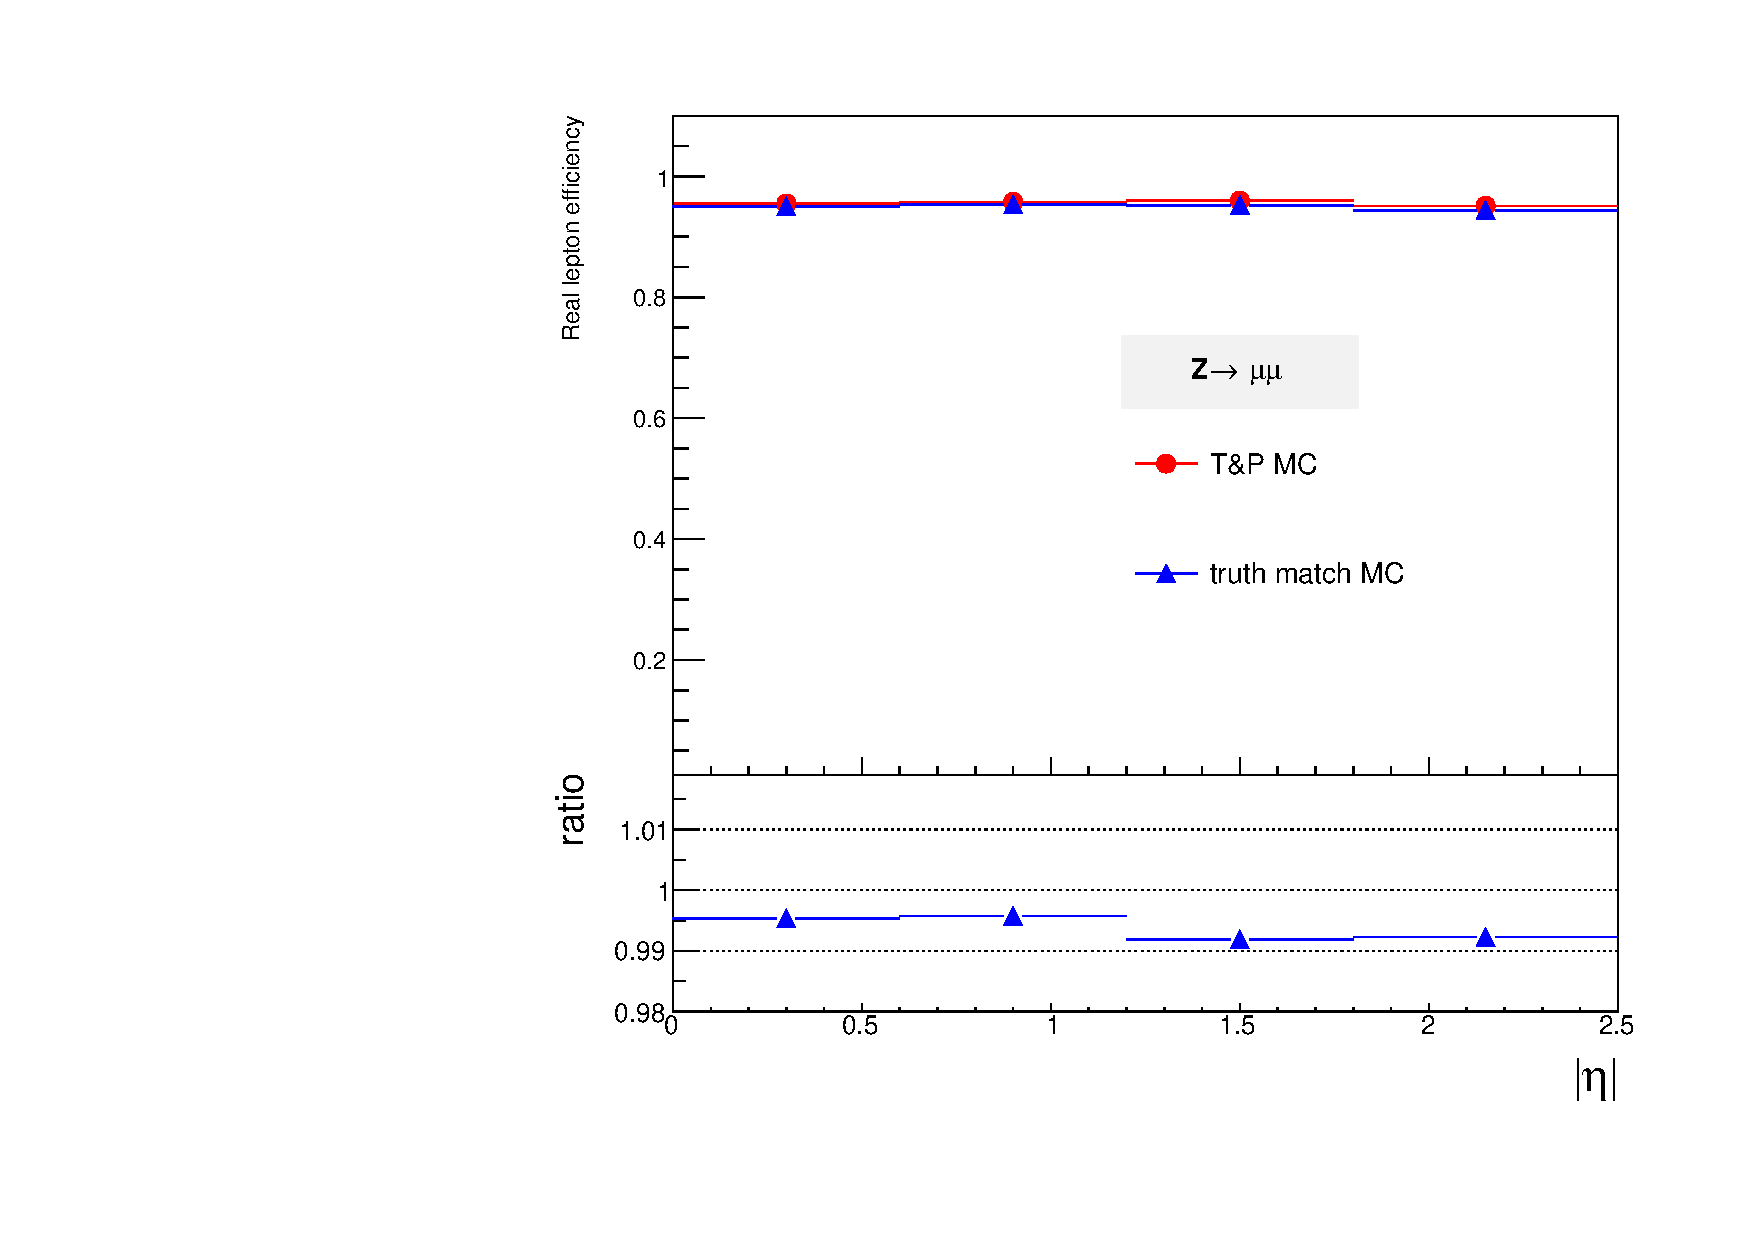
\includegraphics[width=0.32\textwidth]{Compare_TandP_truth_match_muon_eta.pdf}
    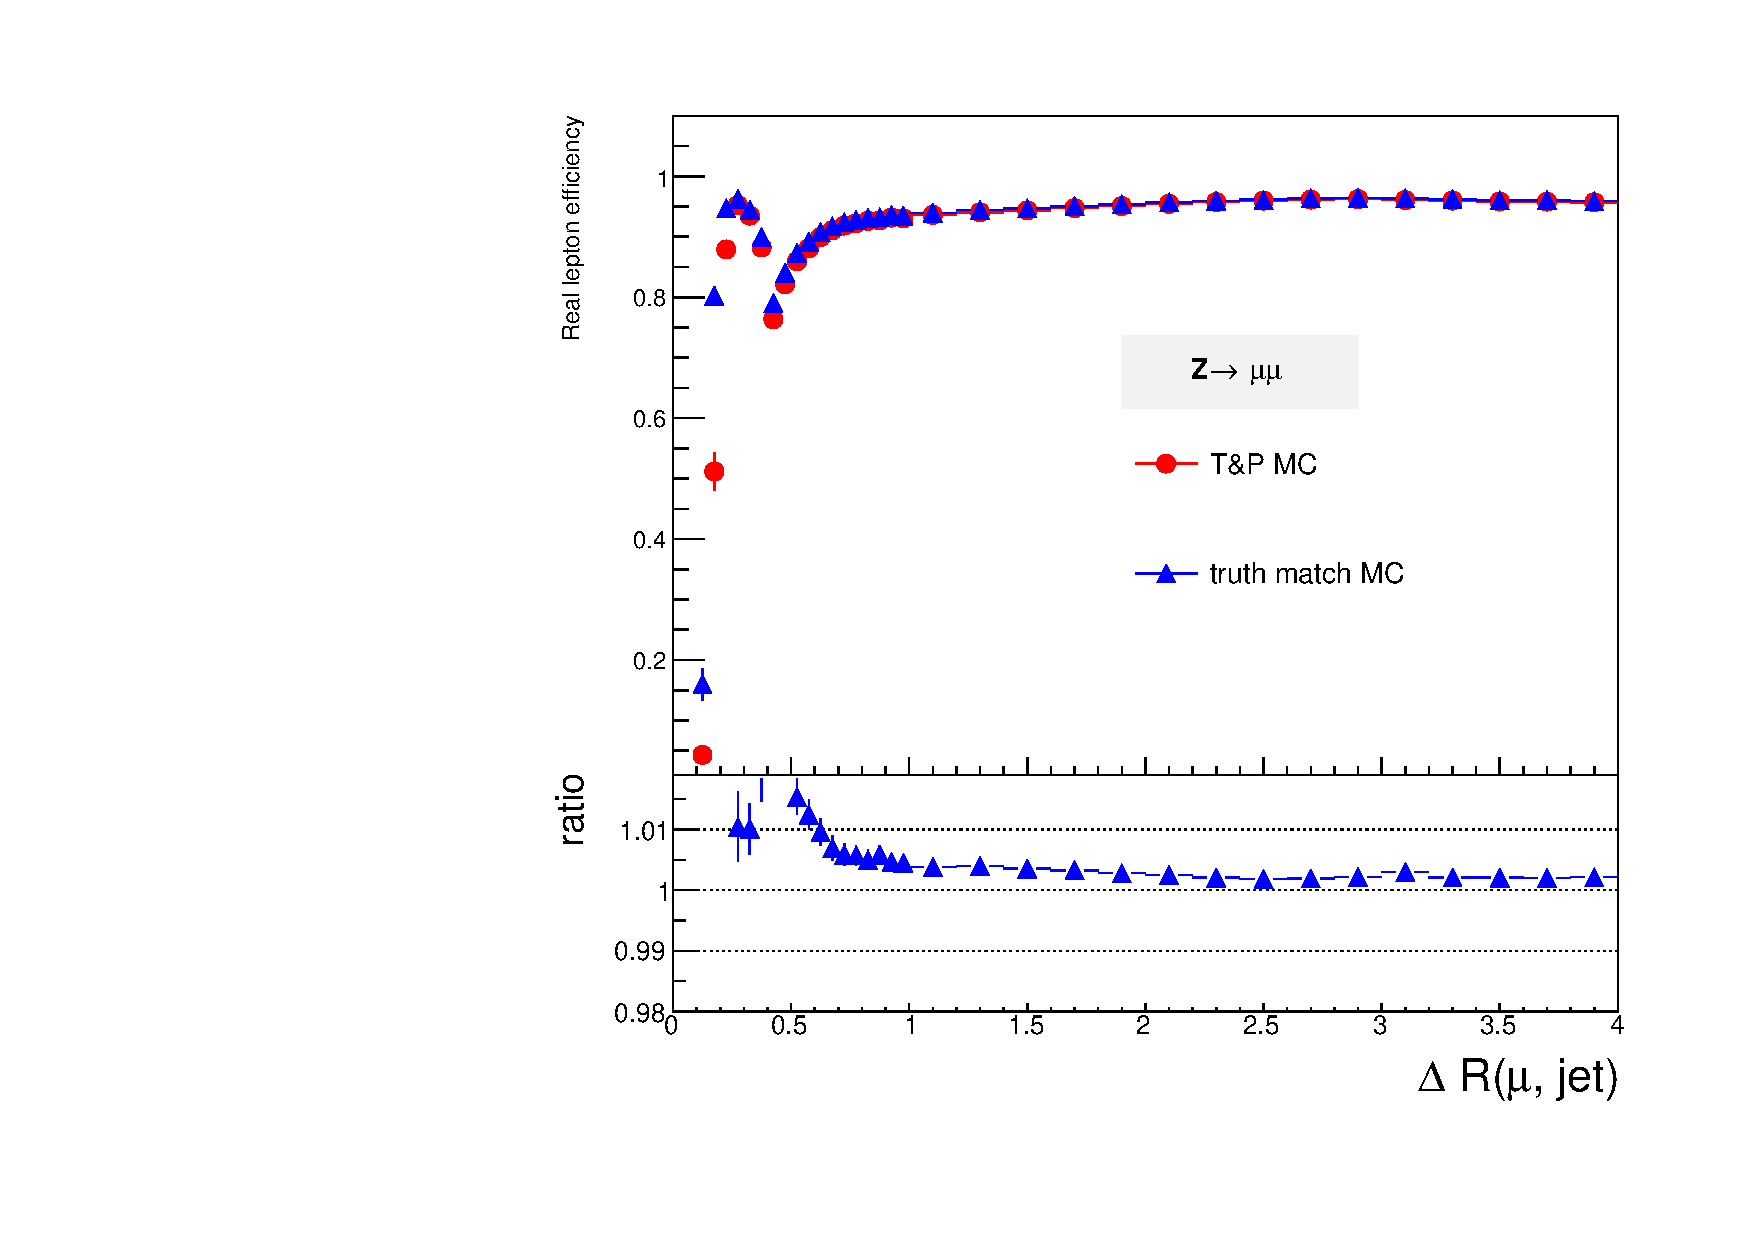
\includegraphics[width=0.32\textwidth]{Compare_TandP_truth_match_muon_dRjet.pdf}
    \caption{The real lepton efficiencies computed by $Z$ tag-and-probe method (red dots) and truth matching (blue triangles).
    The electron cases are on the top row and muon cases are at the bottom row.
    The three columns from the left to the right are the real lepton efficiencies as a function \pt, $|\eta|$, and $\Delta R(\ell, \mathrm{jet})$, respectively.
    The lower pads show the ratio with respect to the $Z$ tag-and-probe method.}
    \label{fig:app_RLE_TandP_truth_match_comparisons}
\end{figure}

\subsection{Tag-and-probe method and truth matching comparisons}
\label{subsec:app_RLE_truth_matched}
The truth matched information in the $Z \to \ell \ell$ MC samples are used to verify the accuracy of $Z$ tag-and-probe method.
Figure~\ref{fig:app_RLE_TandP_truth_match_comparisons} shows the real lepton efficiencies as a function of \pt, $|\eta|$, and $\Delta R(\ell, \mathrm{jet})$ using $Z$ tag-and-probe method and truth matching.
The associated uncertainties are statistical uncertainties only.
For the real electron efficiencies, the largest difference is $\sim$7\% in low \pt and no differences can be seen when $\pt > 50$~{\GeV}; the largest difference is $\sim$3\% in ; the larger differences in $\Delta R(e, \mathrm{jet})$ exist when $\Delta R(e, \mathrm{jet}) < 0.4$.
Because the overlap removal has been applied on the baseline electrons, the $\Delta R(e, \mathrm{jet}) < 0.4$ region lacks statistics.
For the real muon efficiencies, the differences are less then 1\% for \pt and $|\eta|$.
However, the differences are larger for $\Delta R(\mu, \mathrm{jet}) < 0.4$ also because of the overlap removal.
The small differences between two methods indicate the robust of $Z$ tag-and-probe method and the differences may be considered as the systematic uncertainties.

%%%
%%%
%%%

\subsection{Data-to-MC comparisons}
\label{subsec:app_RLE_data_to_mc_comparisons}
The real lepton efficiencies calculating by data and $Z\to \ell\ell$ MC samples are compared.
All 2015 and 2016 data are considered corresponding to an integrated luminosity of 36.5~\ifb.
All the lepton scale factors are applied on the MC samples and the simulation is re-weighted to the pileup observed in data.
Figure~\ref{fig:app_RLE_real_efficiency_pt_eta_dRjet} shows the real efficiencies as a function of \pt, $|\eta|$ and $\Delta R(\ell, \mathrm{jet})$ using data and $Z\to \ell \ell$ MC samples, respectively.
The associated uncertainties are statistical uncertainties only.
Good agreement between data and MC can be seen in the \pt and $|\eta|$ plots.
Larger differences exist in $\Delta R(\ell, \mathrm{jet})$ plots because of lacking statistics.

\begin{figure}[htb]
    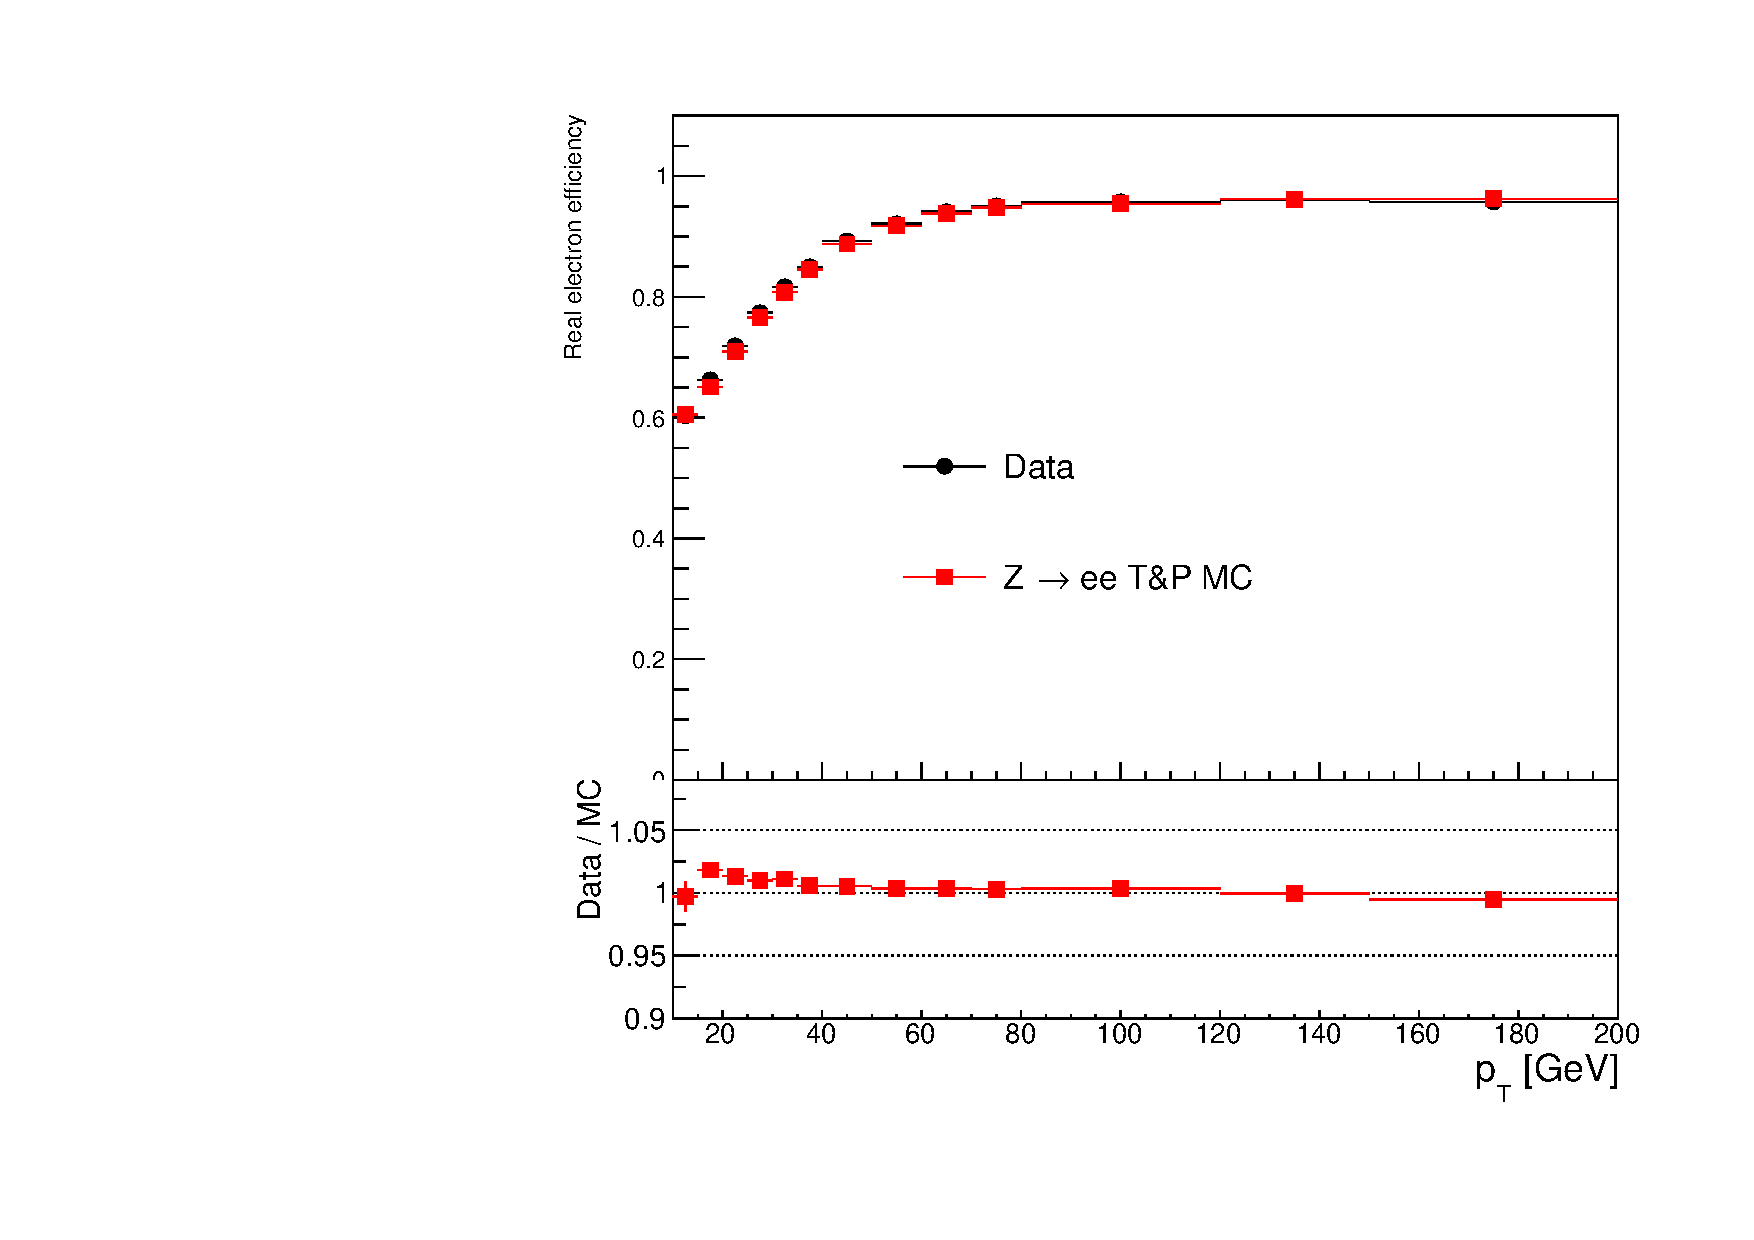
\includegraphics[width=0.32\textwidth]{real_efficiency_ratio_plot_electron_pt.pdf}
    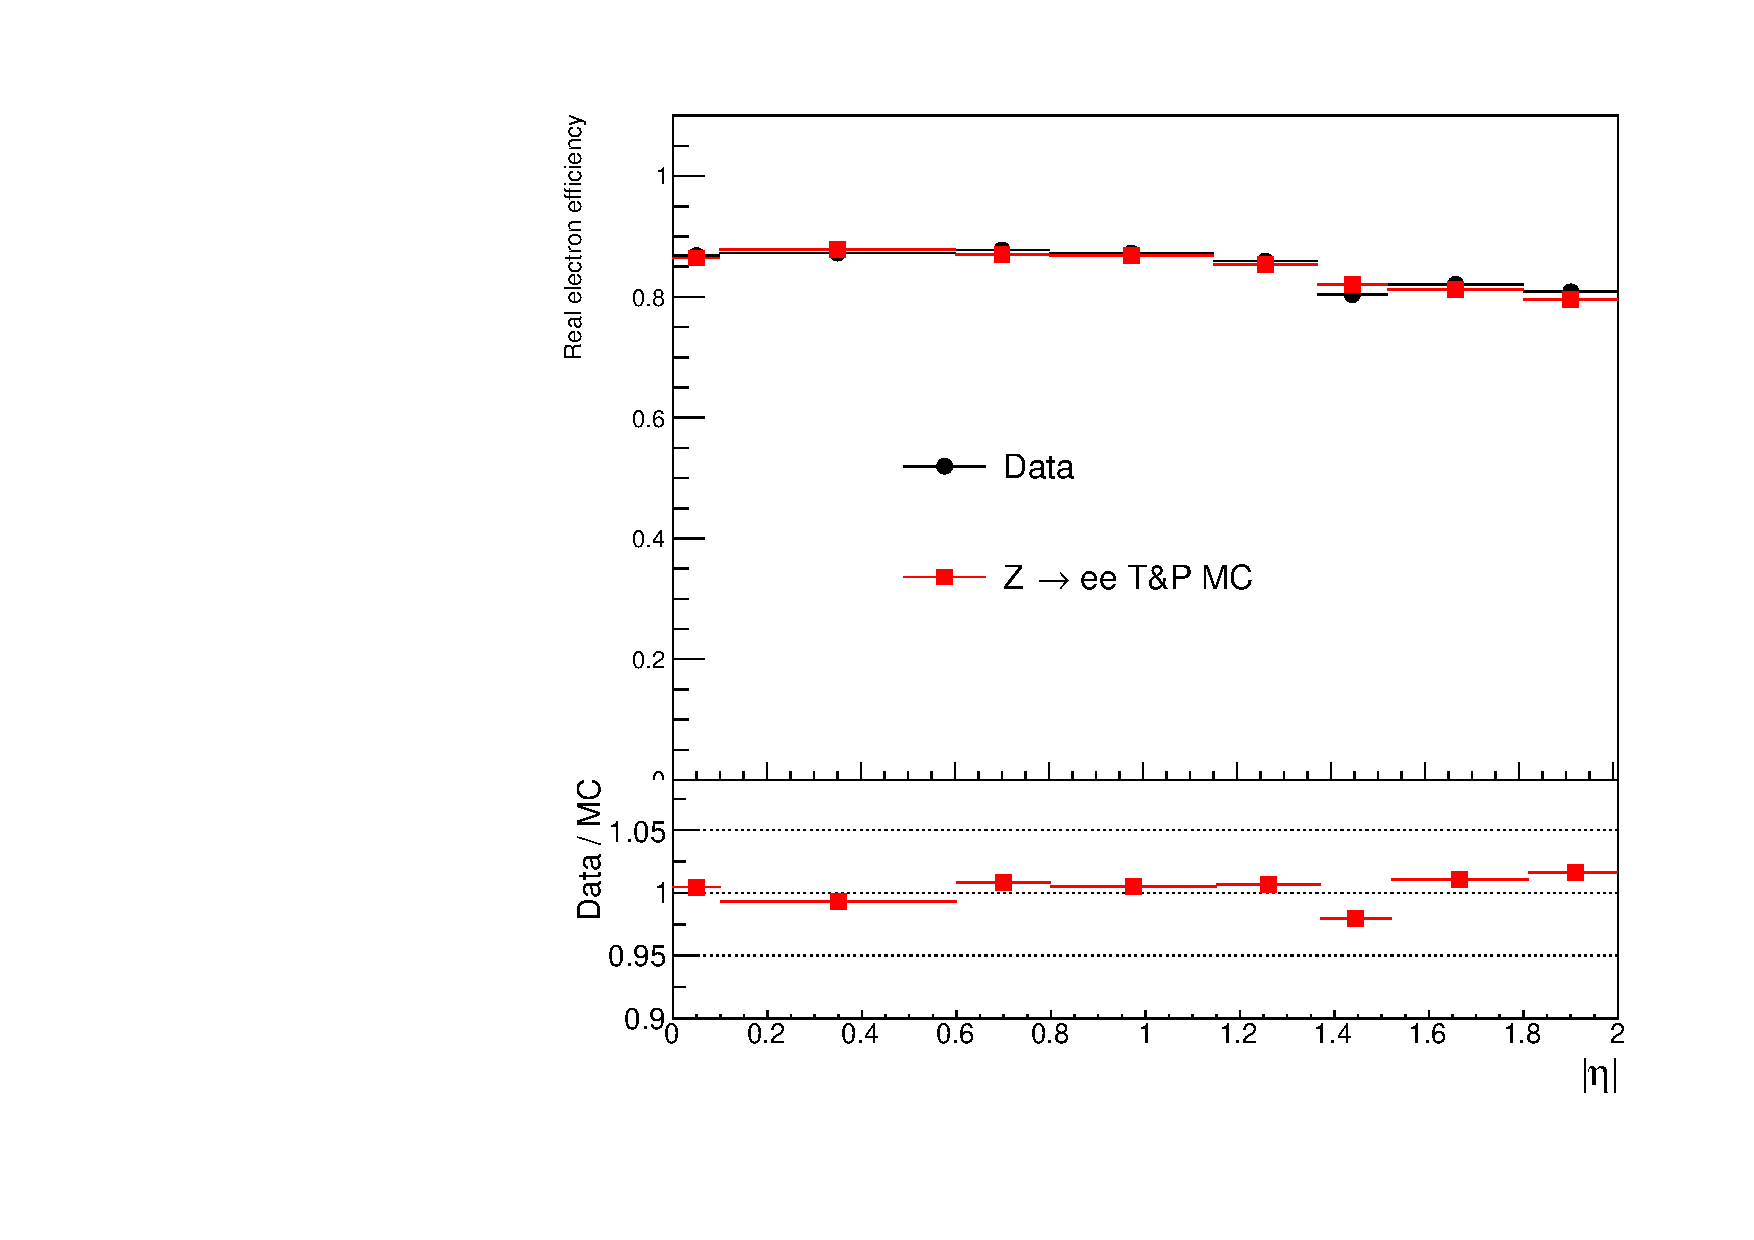
\includegraphics[width=0.32\textwidth]{real_efficiency_ratio_plot_electron_eta.pdf}
    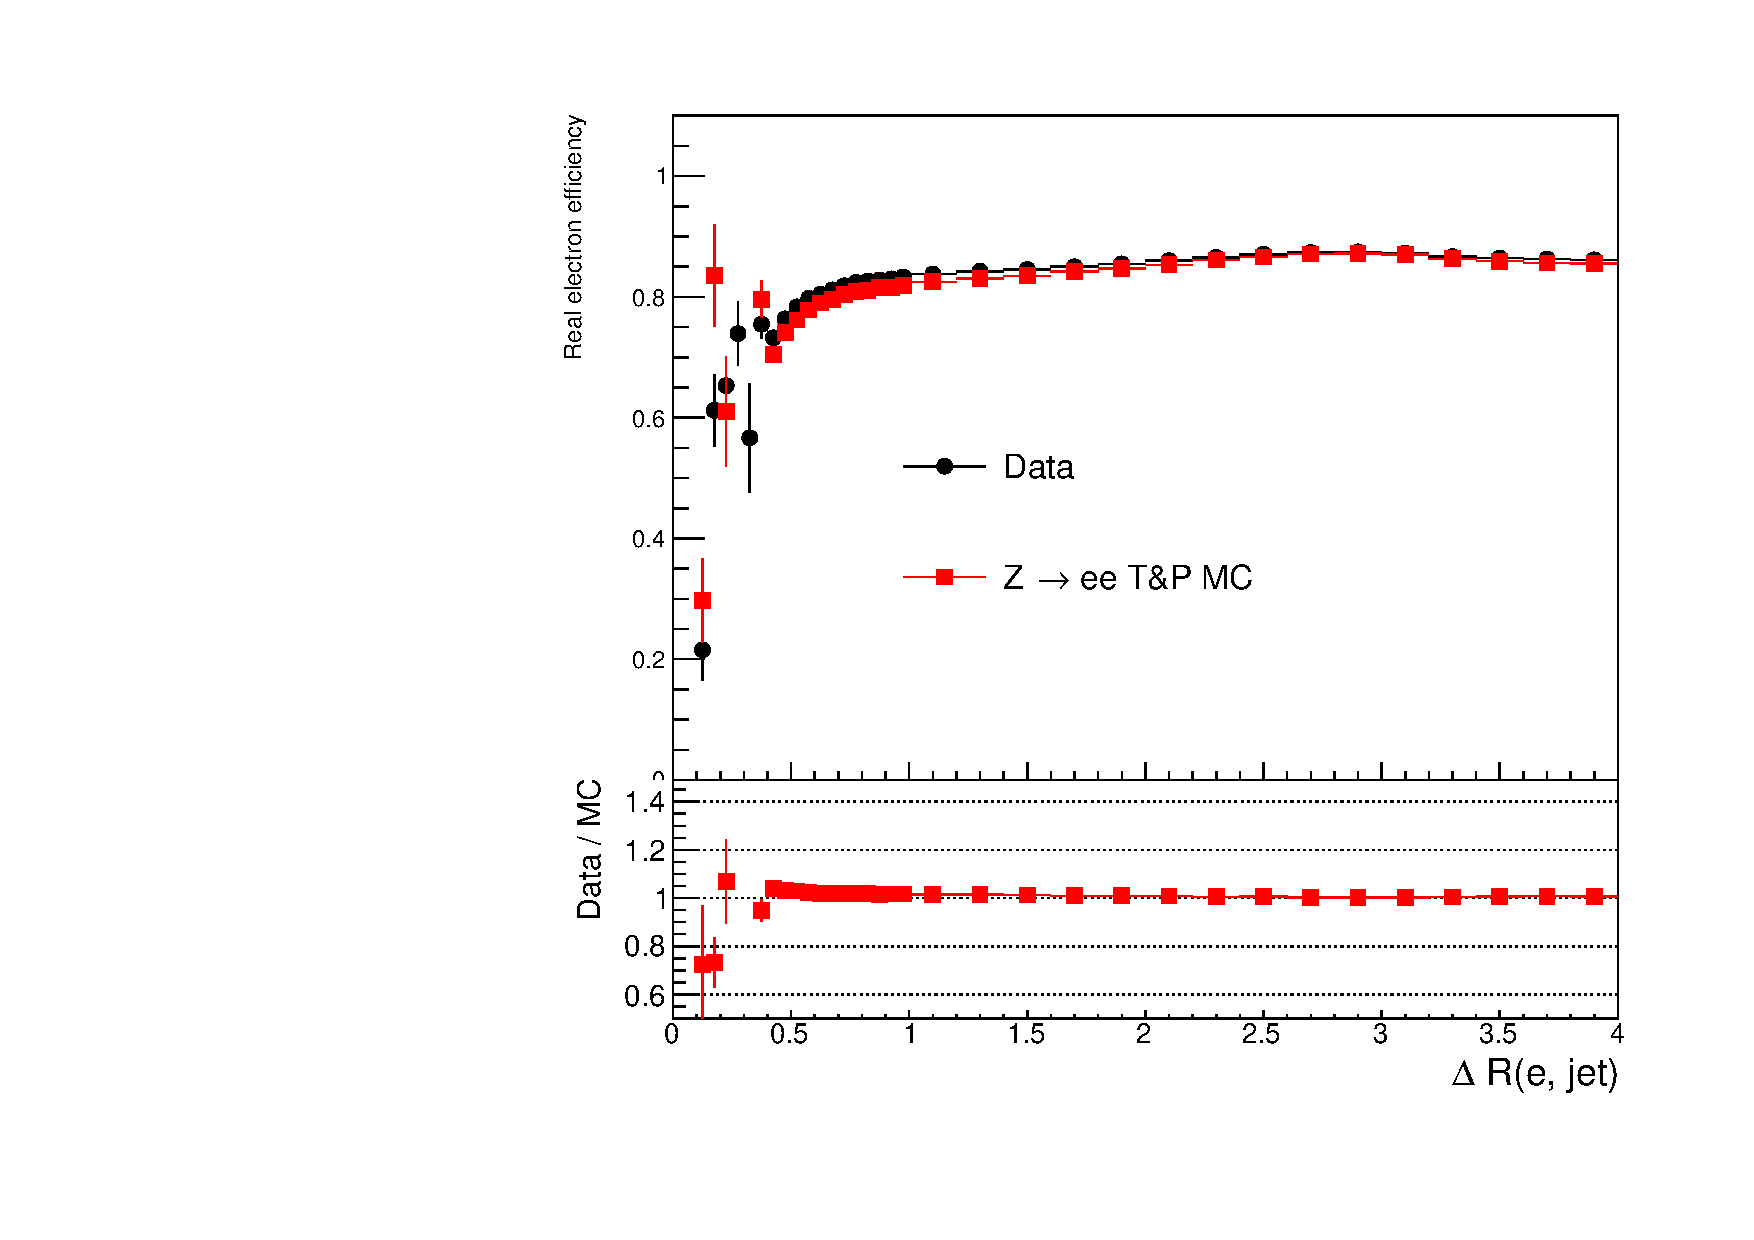
\includegraphics[width=0.32\textwidth]{real_efficiency_ratio_plot_electron_dRjet.pdf}\\
    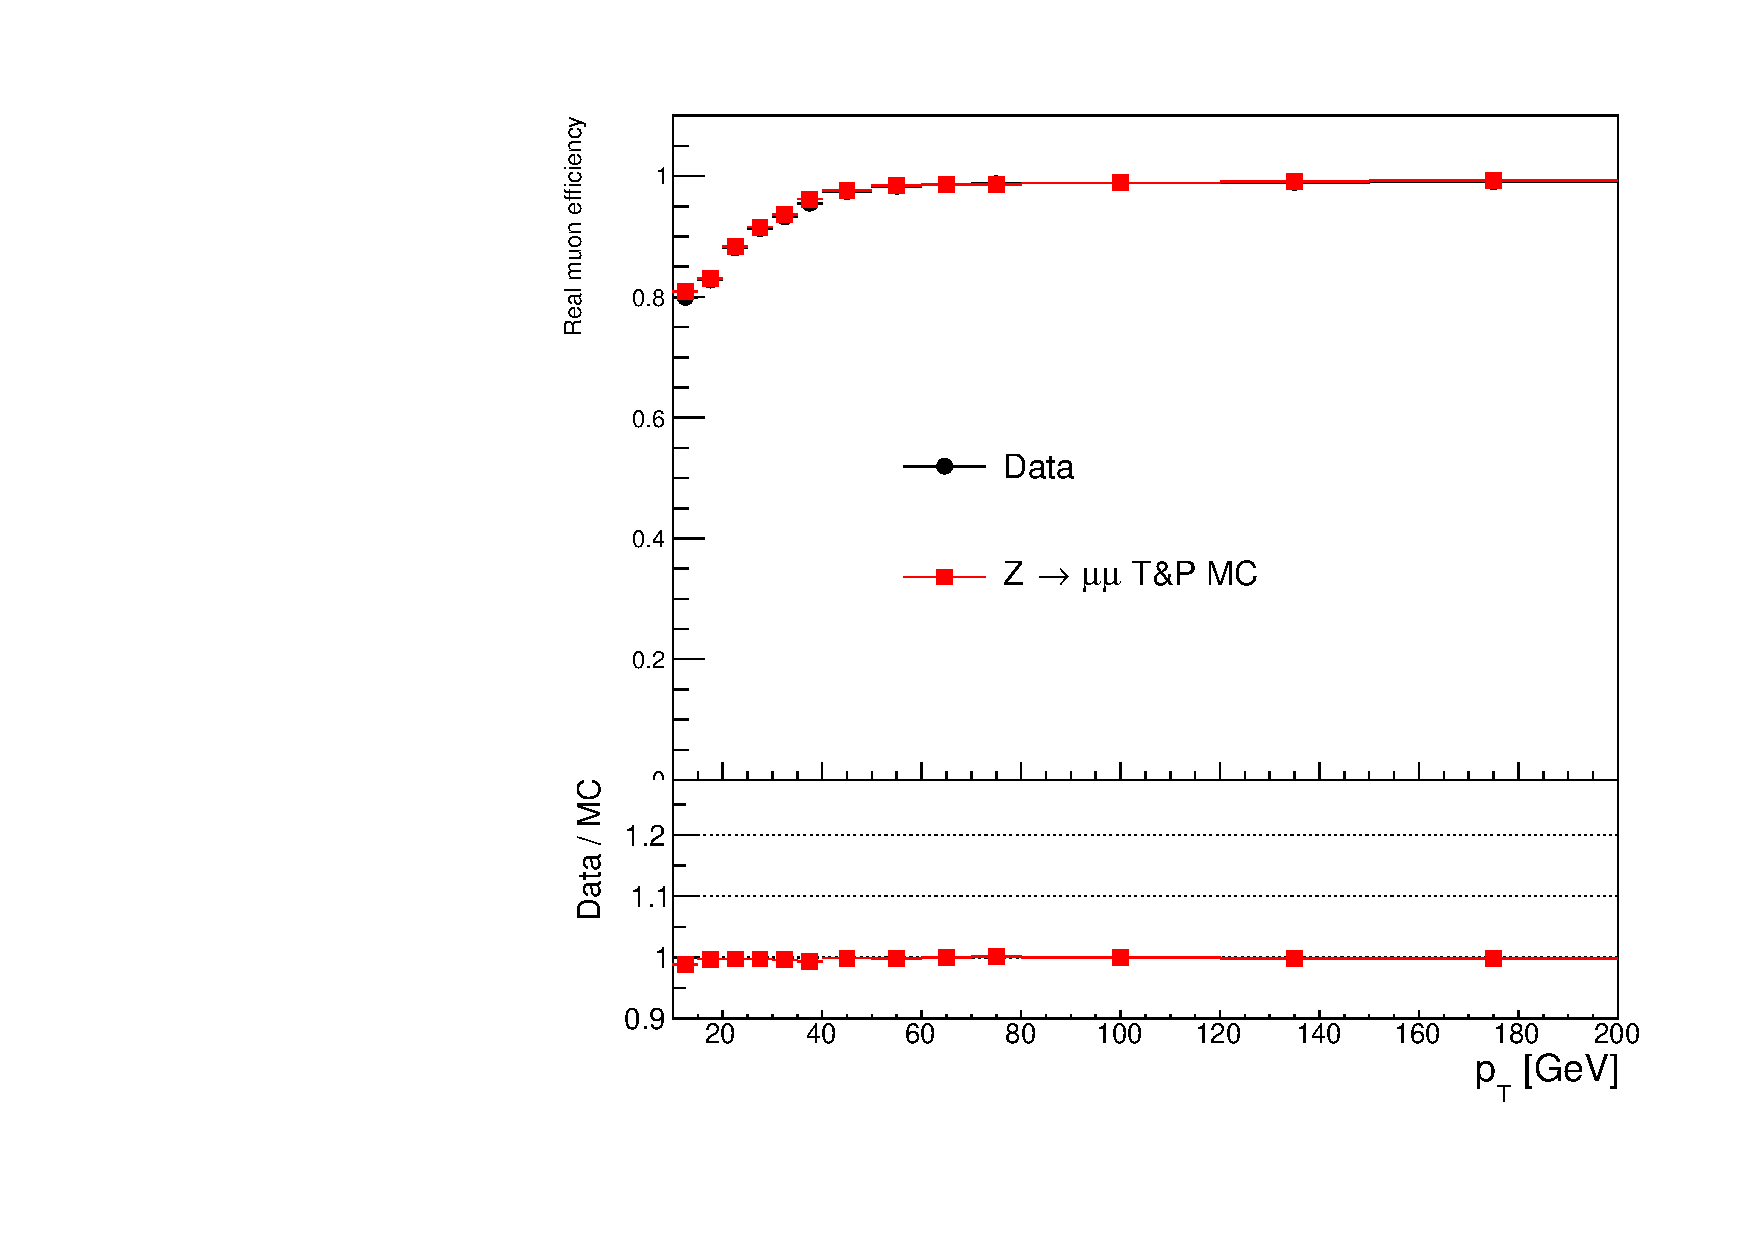
\includegraphics[width=0.32\textwidth]{real_efficiency_ratio_plot_muon_pt.pdf}
    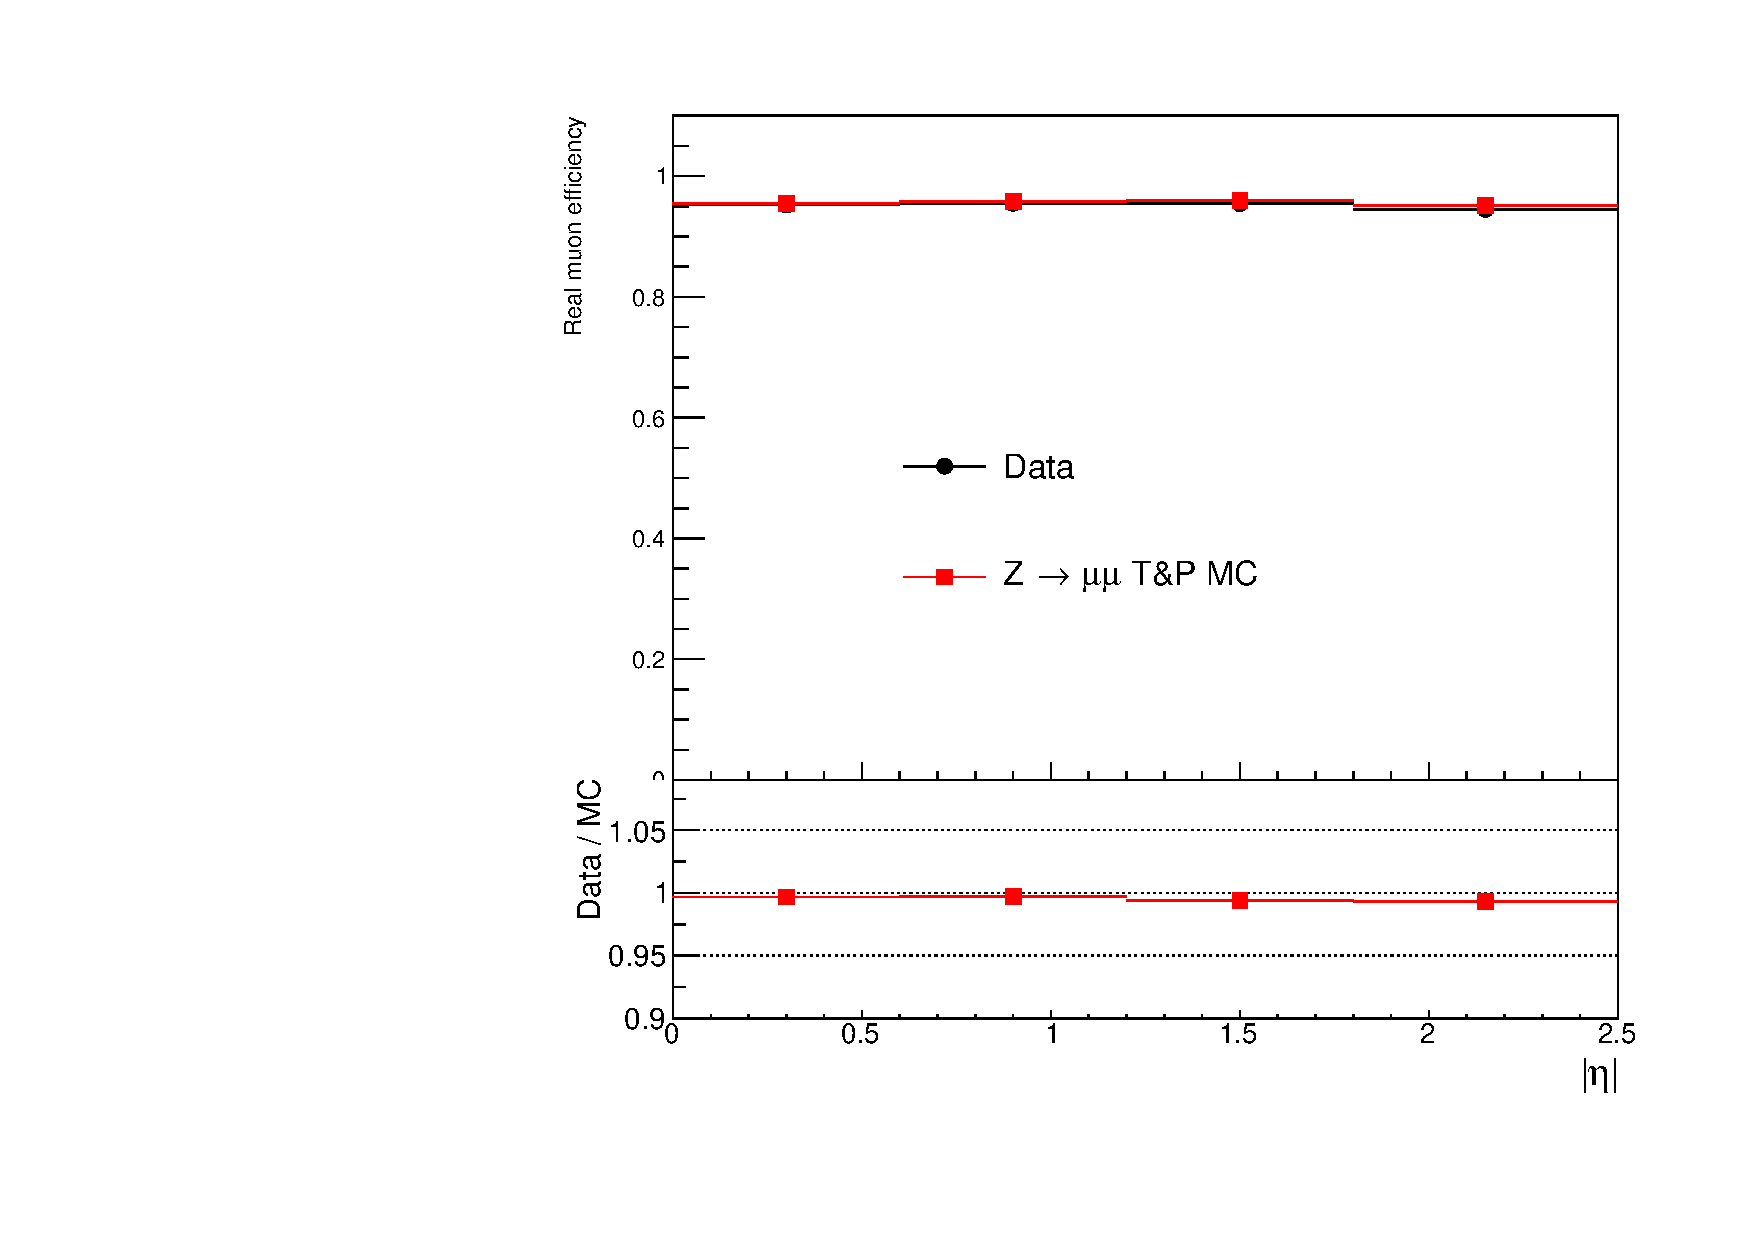
\includegraphics[width=0.32\textwidth]{real_efficiency_ratio_plot_muon_eta.pdf}
    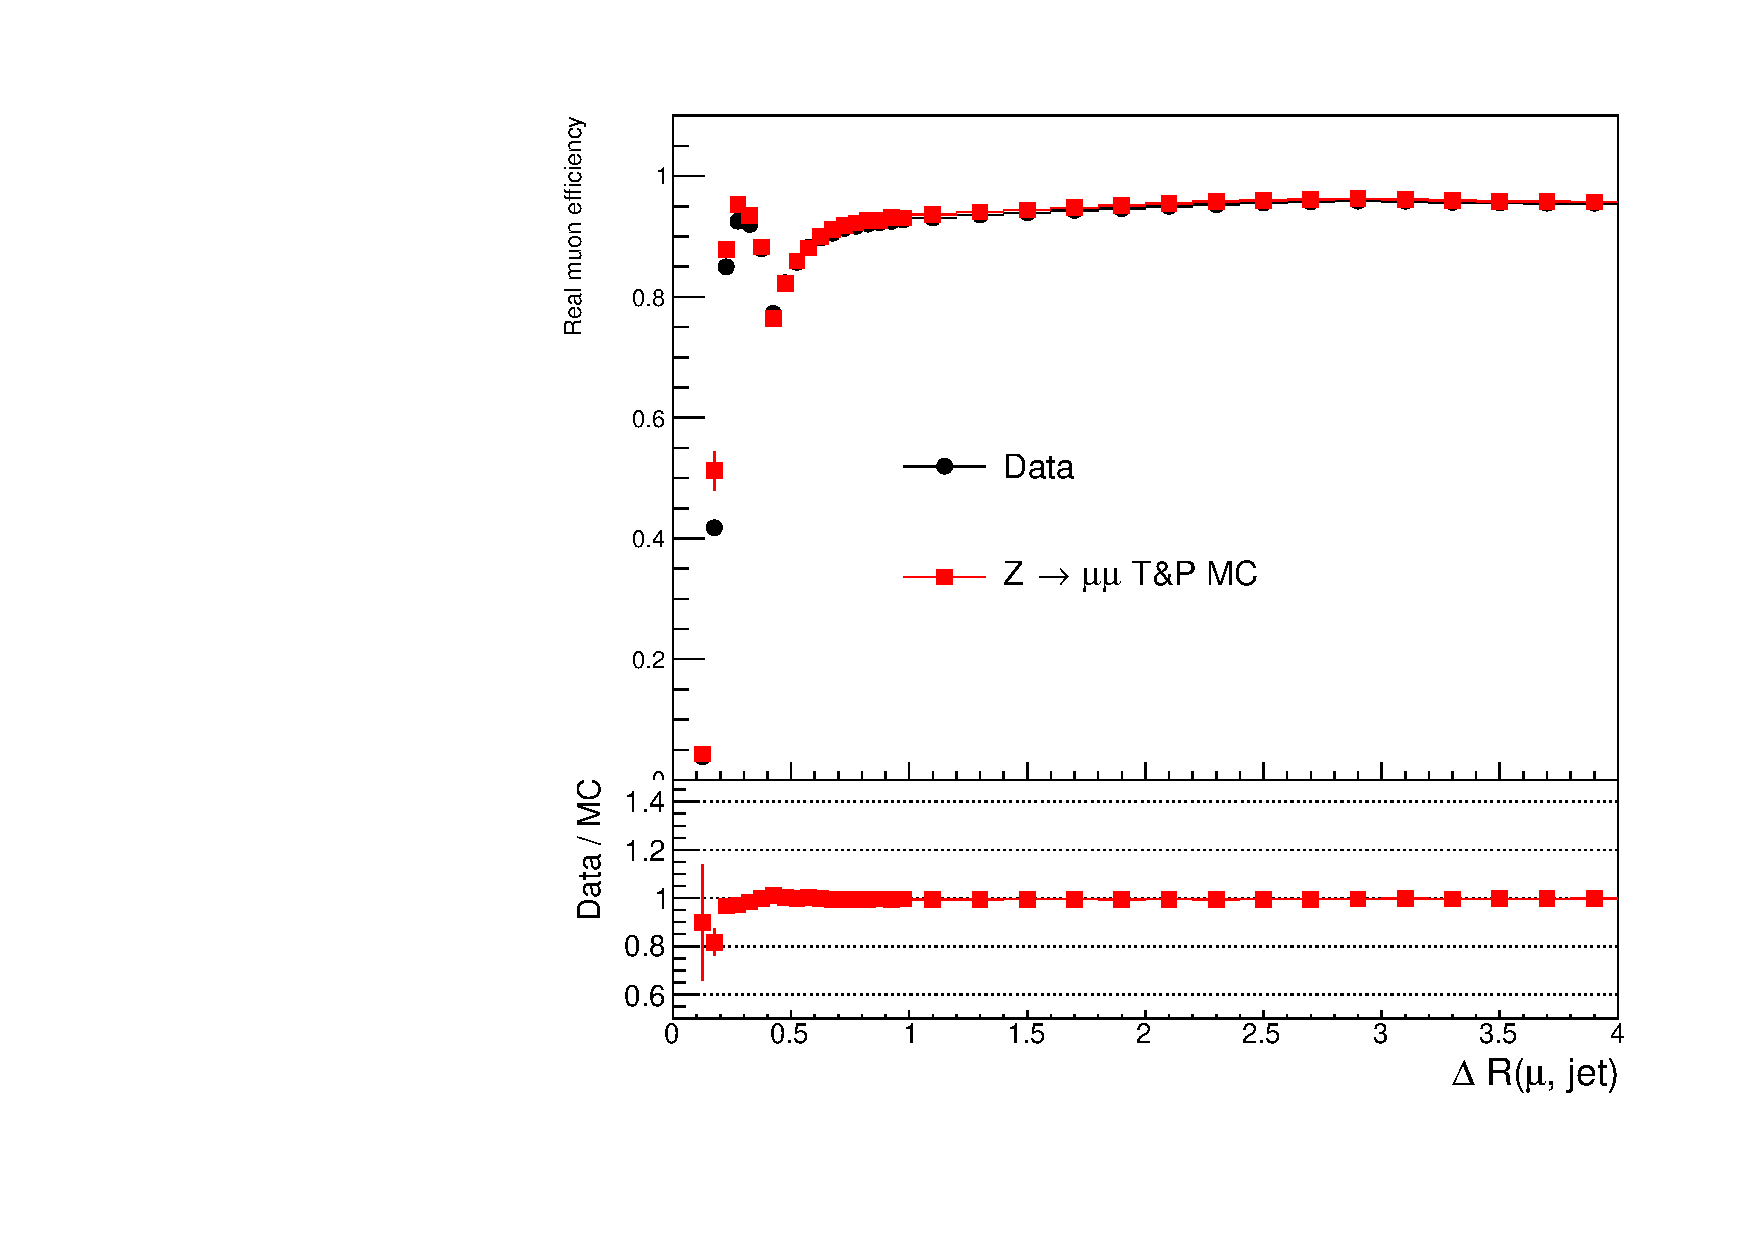
\includegraphics[width=0.32\textwidth]{real_efficiency_ratio_plot_muon_dRjet.pdf}
    \caption{The real lepton efficiencies measured on 2015 + 2016 data (black dots) and $Z\to \ell\ell$ MC samples (red squares) using the $Z$ tag-and-probe method.
    The electron cases are on the top row and muon cases are at the bottom row.
    The three columns from the left to the right are the real lepton efficiencies as a function \pt, $|\eta|$, and $\Delta R(\ell, \mathrm{jet})$, respectively.
    The MC samples have been re-weighted to the pileup observed in data.}
    \label{fig:app_RLE_real_efficiency_pt_eta_dRjet}
\end{figure}

%%%
%%%
%%%

\subsection{Real lepton efficiency versus pileup}
\label{subsec:app_RLE_vs_pileup}
The relations between the real lepton efficiencies and the pileup are also studied.
The efficiencies computed by 2015 + 2016 data, $Z$ tag-and-probe method and truth matching MC samples are shown in Fig.~\ref{fig:app_RLE_vs_pileup}.

\begin{figure}[htb]
    \begin{subfigure}[b]{0.48\textwidth}
        \begin{center}
            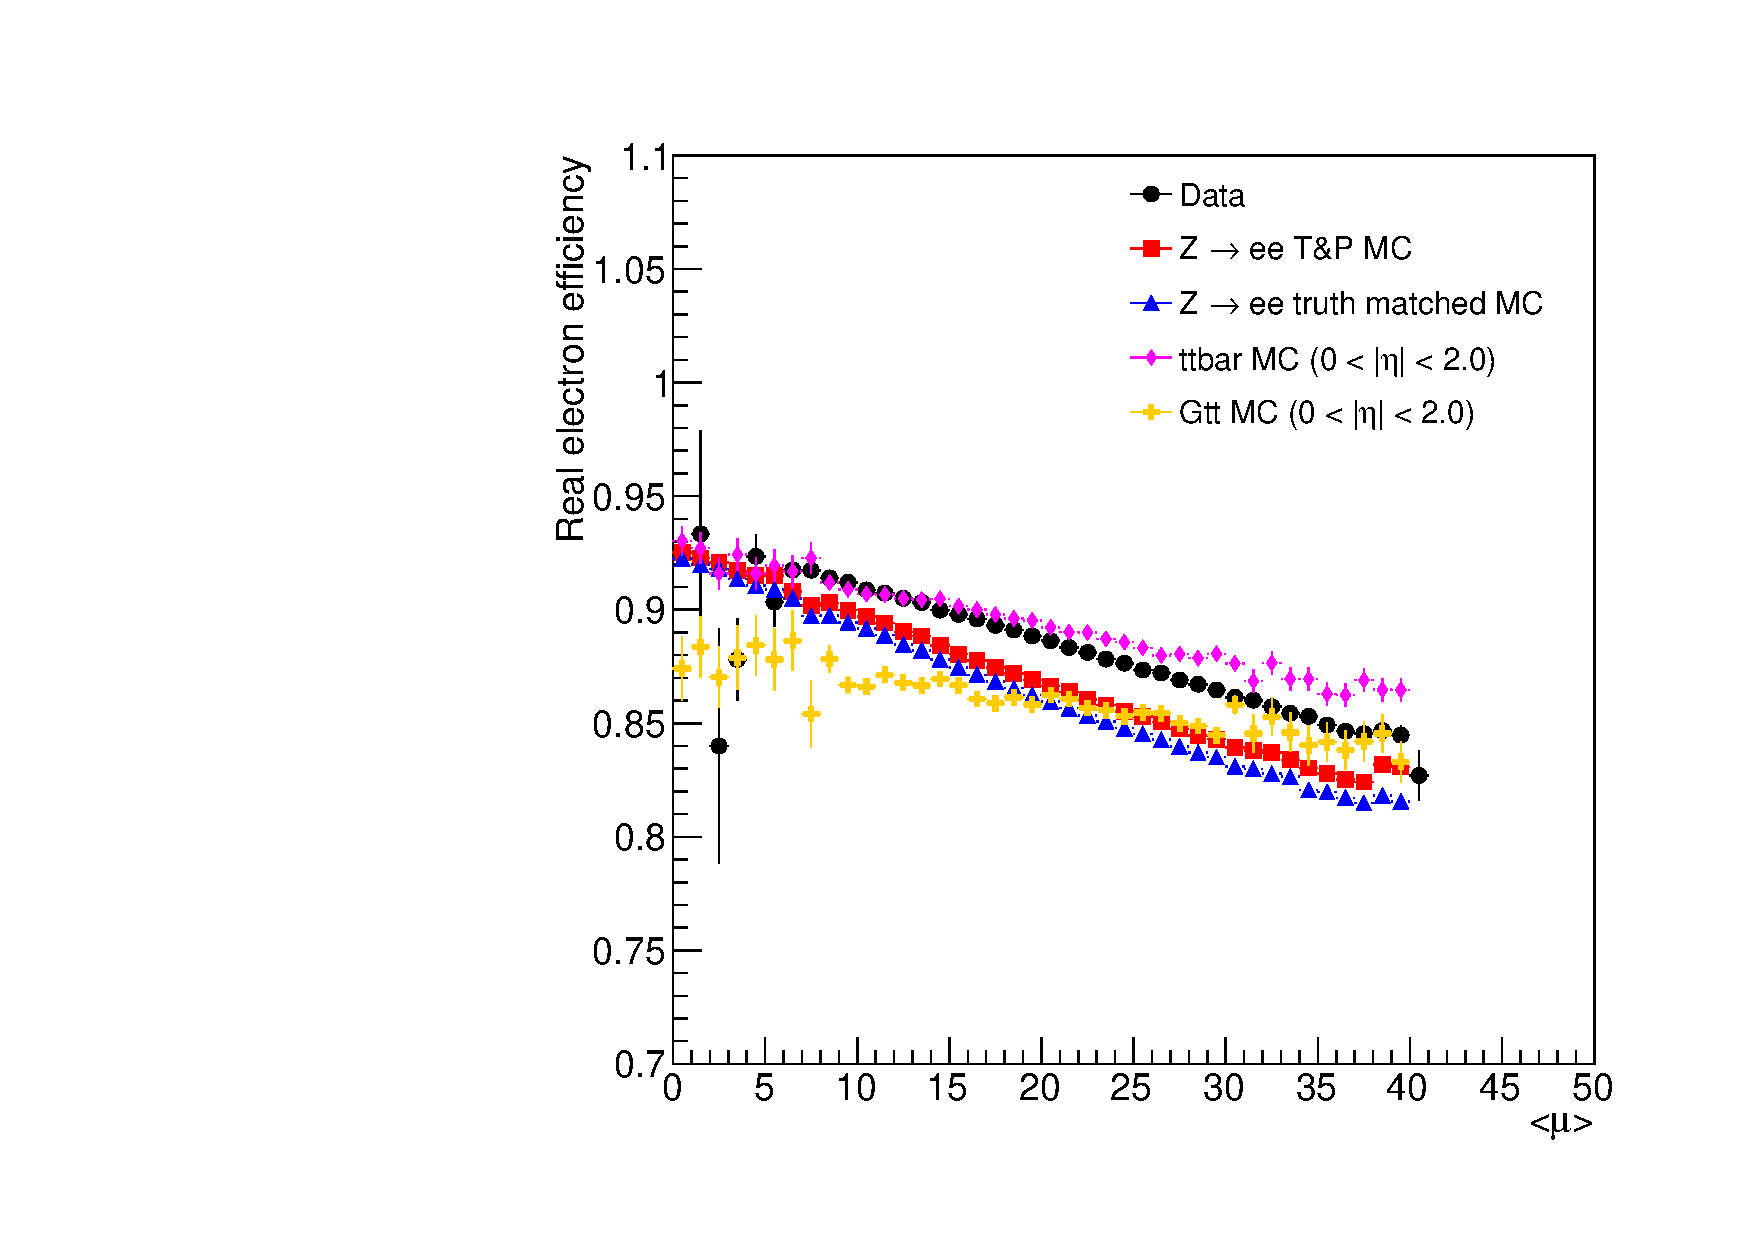
\includegraphics[scale=0.35]{real_efficiency_vs_AvgMu_elec.pdf}
            \caption{Electron}
        \end{center}
    \end{subfigure}
    \begin{subfigure}[b]{0.48\textwidth}
        \begin{center}
            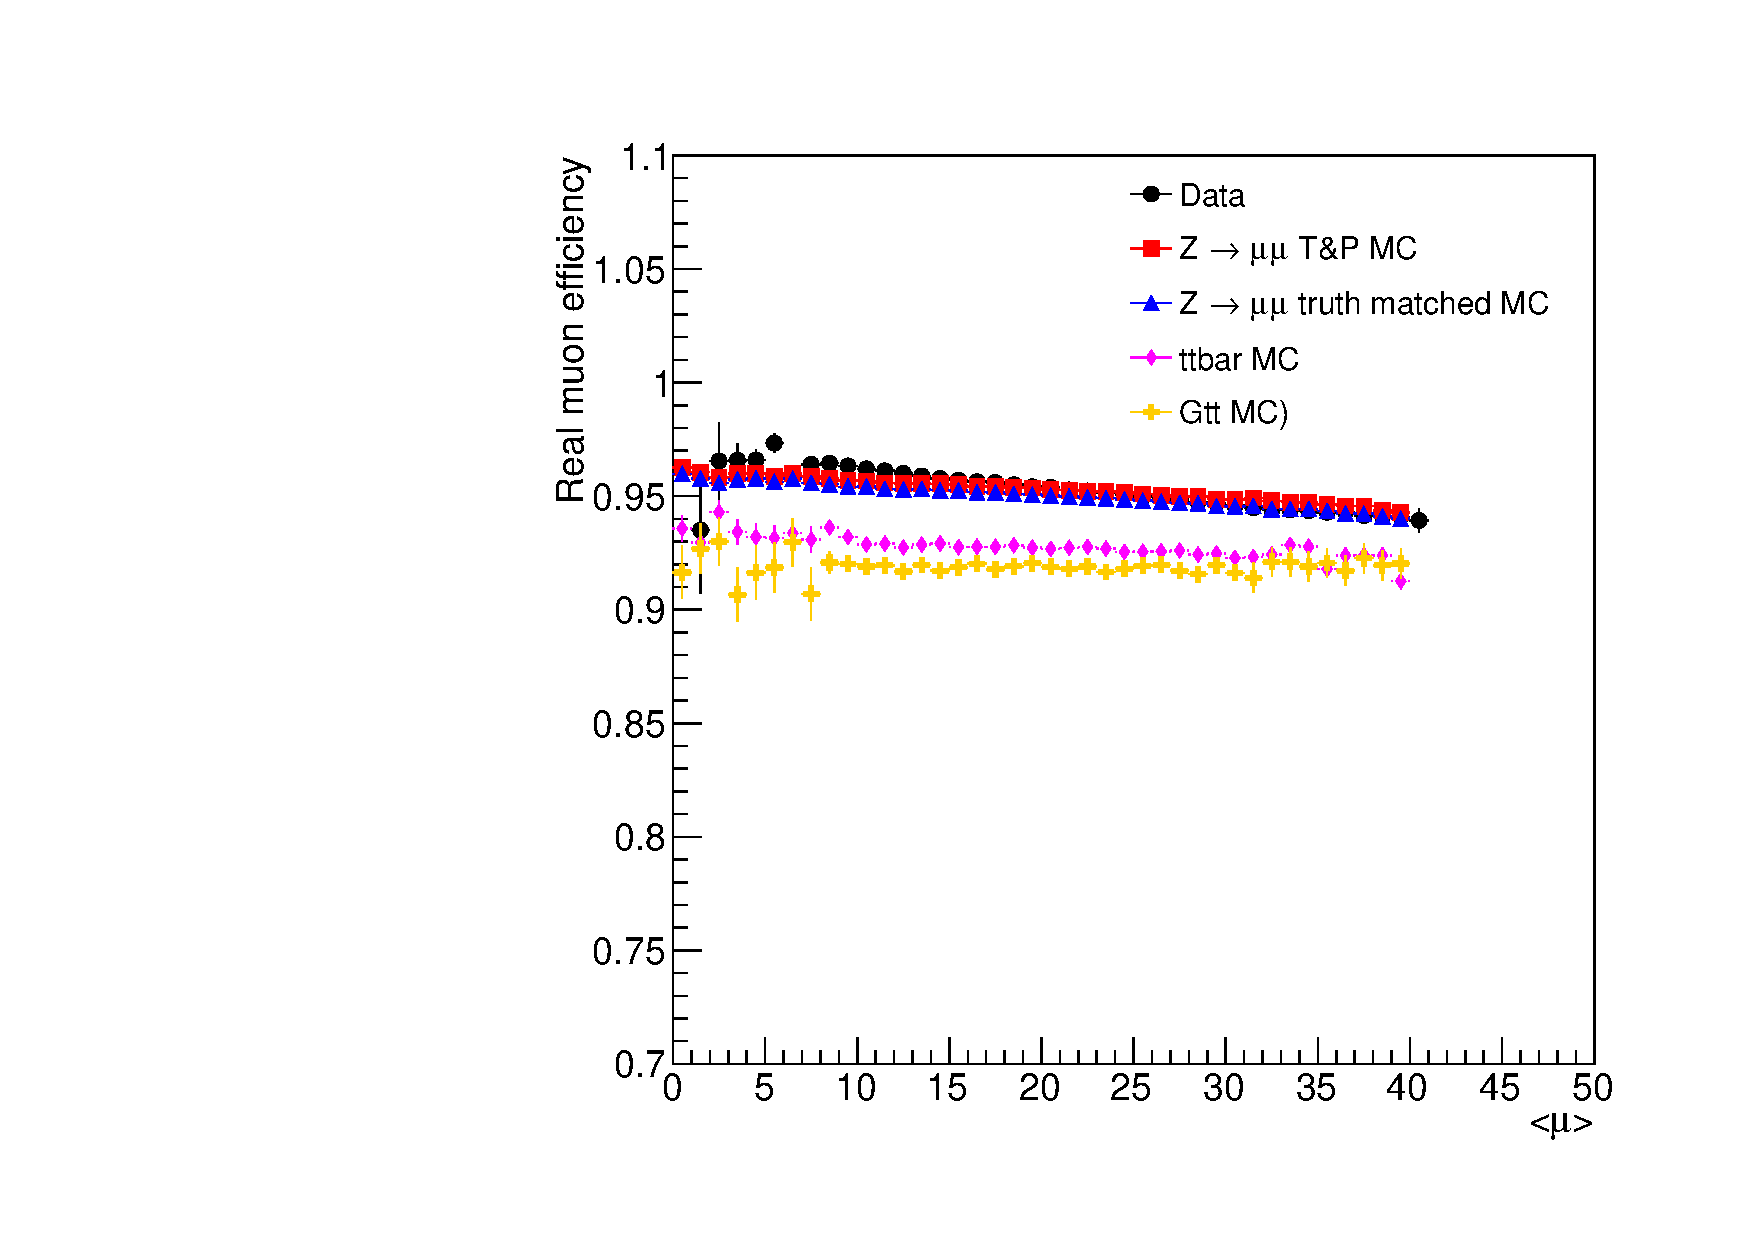
\includegraphics[scale=0.35]{real_efficiency_vs_AvgMu_muon.pdf}
            \caption{Muon}
        \end{center}
    \end{subfigure}
    \caption{The real lepton efficiencies as a function of the average interactions per crossing $<\mu>$.
    The data is presented in black dots,  $Z\to \ell\ell$ tag-and-probe is presented in red squares, the truth matching is presented in blue triangles, the \ttbar is presented in magenta diamonds, and $\tilde{g} \to \ttbar \widetilde{\chi^{0}_{1}}$ is presented in yellow crosses.
    The $|\eta|<2$ requirement has been applied on the \ttbar and $\tilde{g} \to \ttbar \widetilde{\chi^{0}_{1}}$ MC samples for the electron case.}
\label{fig:app_RLE_vs_pileup}
\end{figure}

In order to study the efficiencies with different event topologies, the \ttbar and $\tilde{g} \to \ttbar \widetilde{\chi^{0}_{1}}$ MC samples are considered.
The real electron efficiencies are $\sim$92\% at low $<\mu>$ and decrease when $<\mu>$ increases.
The measured real lepton efficiencies using $\tilde{g} \to \ttbar \widetilde{\chi^{0}_{1}}$ MC sample is lower then the data case.
The \ttbar and data have similar real electron efficiencies.
However, the real muon efficiencies for \ttbar is lower than the data because the efficiencies in $\pt < 40$~{\GeV} is lower.
If a $\pt > 40$~{\GeV} requirement is applied on the \ttbar MC sample, then the efficiencies are agreed with data.
Figure~\ref{fig:app_RLE_real_efficiency_ttbar_gtt} shows the measured real electron and muon efficiencies as a function of $\pt$ using data, $Z$ tag-and-probe method, truth matching, \ttbar, and $\tilde{g} \to \ttbar \widetilde{\chi^{0}_{1}}$ MC samples.
The real lepton efficiencies of \ttbar process is lower than the data one in $\pt < 40$~{\GeV} region.
The real lepton efficiencies of $\tilde{g} \to \ttbar \widetilde{\chi^{0}_{1}}$ process are lower than data in both electron and muon cases.

\begin{figure}[htb]
    \begin{subfigure}[b]{0.48\textwidth}
        \begin{center}
            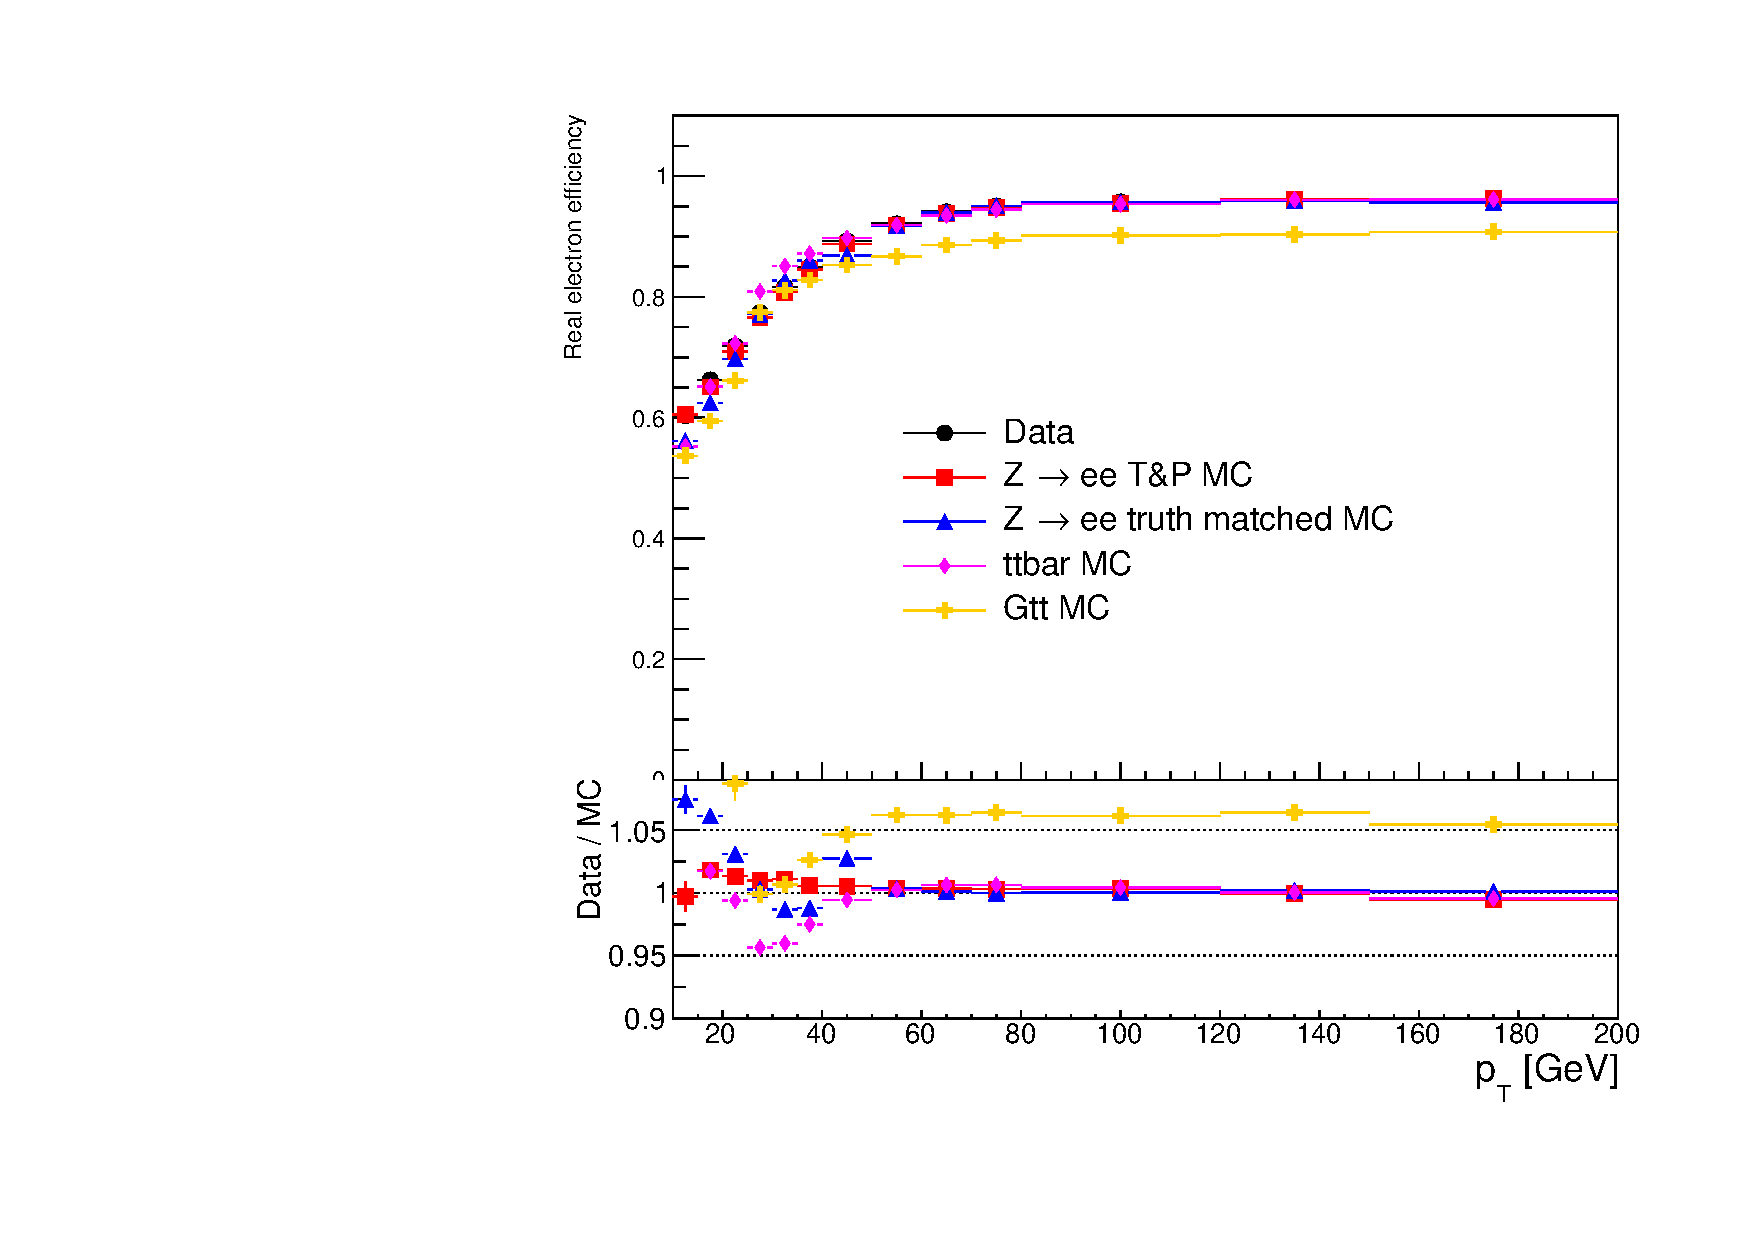
\includegraphics[scale=0.35]{real_efficiency_ratio_plot_electron_pt_ttbar_gtt.pdf}
            \caption{Electron}
        \end{center}
    \end{subfigure}
    \begin{subfigure}[b]{0.48\textwidth}
        \begin{center}
            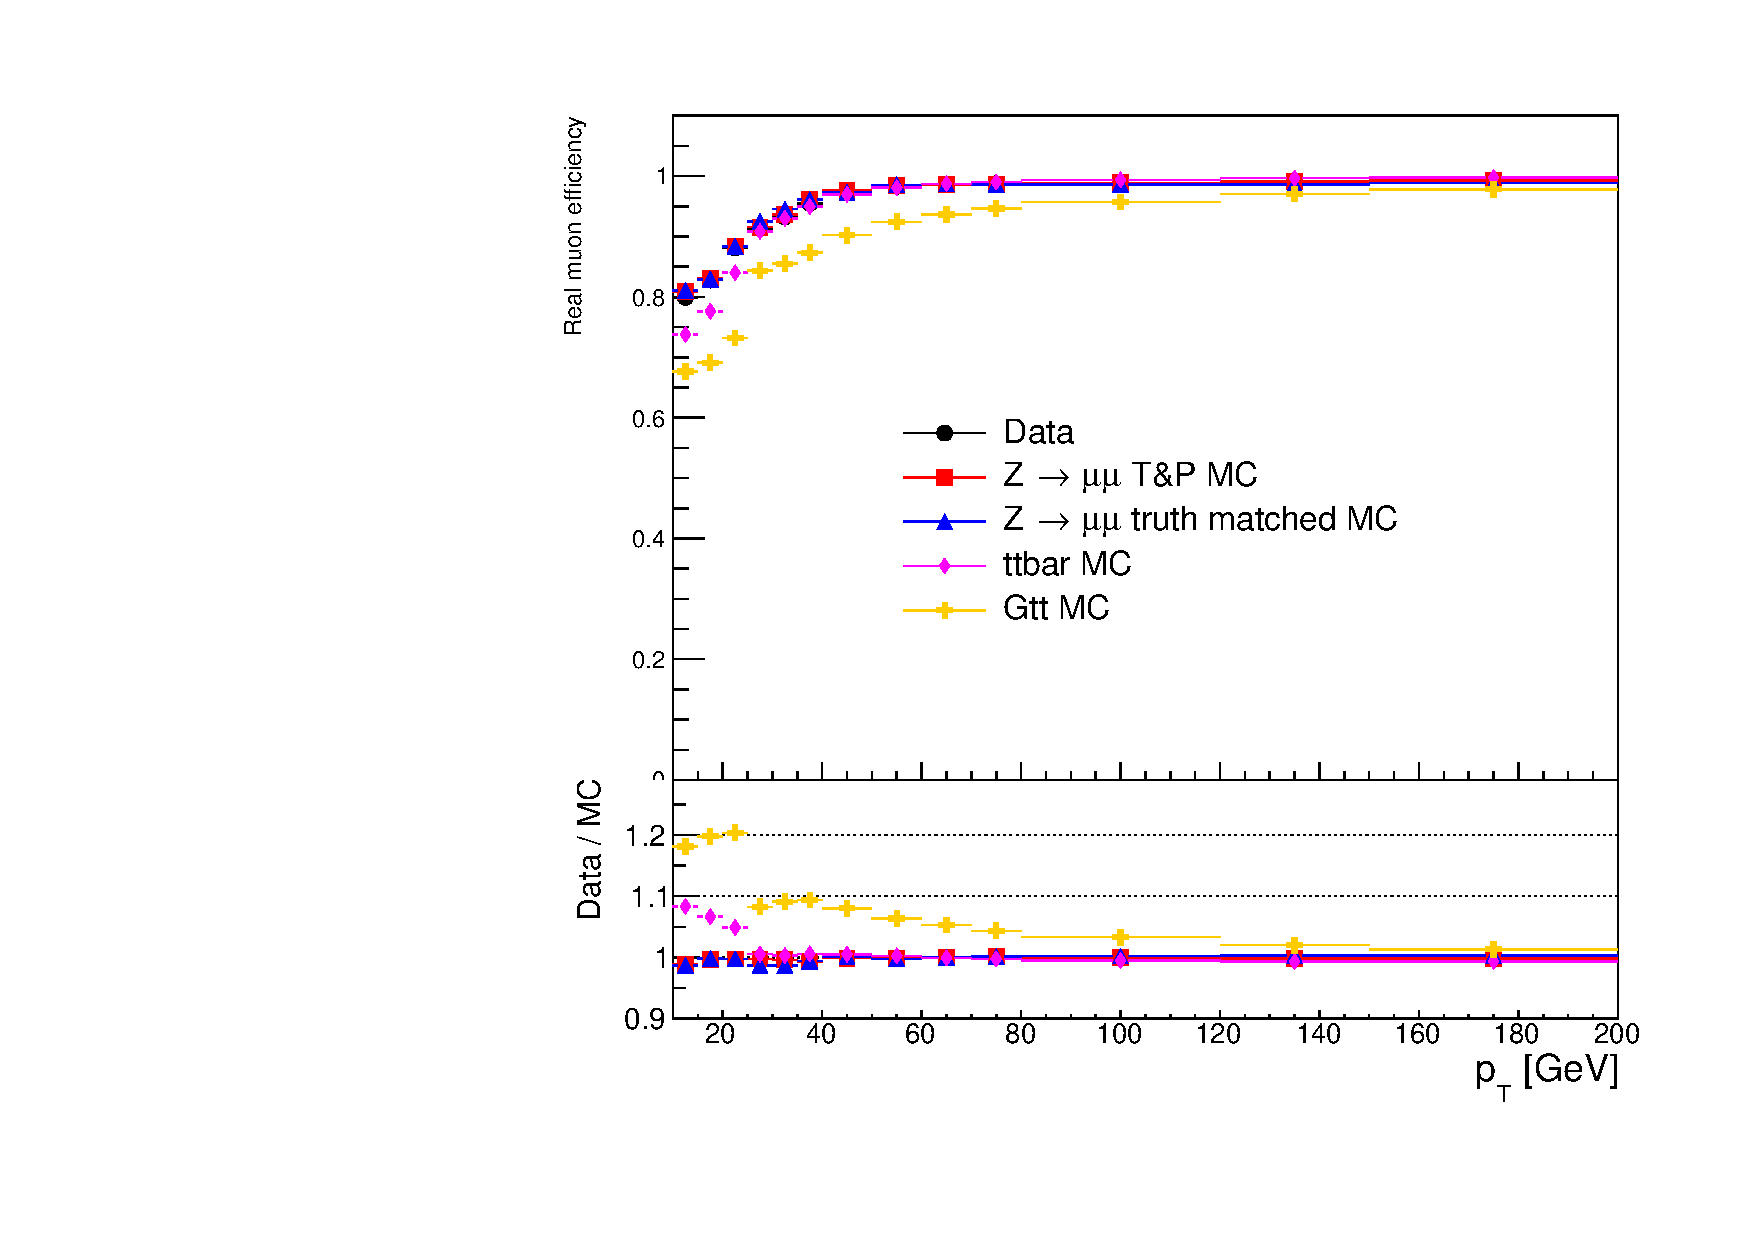
\includegraphics[scale=0.35]{real_efficiency_ratio_plot_muon_pt_ttbar_gtt.pdf}
            \caption{Muon}
        \end{center}
    \end{subfigure}
    \caption{The real electron and muon efficiencies as a function of $\pt$.
    The data is presented in black dots,  $Z\to \ell\ell$ tag-and-probe is presented in red squares, the truth matching is presented in blue triangles, the \ttbar is presented in magenta diamonds, and $\tilde{g} \to \ttbar \widetilde{\chi^{0}_{1}}$ is presented in yellow crosses.
    The differences in the $\pt < 40$~{\GeV} region come from the different event topologies.}
    \label{fig:app_RLE_real_efficiency_ttbar_gtt}
\end{figure}

%%%
%%%
%%%

\section{Sources of systematic uncertainties}
\label{sec:app_RLE_sources_of_systematic_uncertainties}

%%%
%%%
%%%

\subsection{Measurement systematics}
\label{subsec:app_RLE_bkg_systematics}
The measurement systematic uncertainties of the real lepton efficiency calculated by the $Z$ tag-and-probe method have been studied by varying the background template definitions, the template fitting ranges, and the $m_{\ell \ell}$ windows.
The definition of 3 background templates are listed in Table~\ref{tab:app_RLE_bkg_templates}.
The additional template fitting ranges are [60 \textendash 70] $\cup$ [100 \textendash 120]~{\GeV} and [65 \textendash 75] $\cup$ [100 \textendash 120]~{\GeV}.
The two other $m_{\ell \ell}$ windows considered are $75 < m_{ee} < 105$~{\GeV} and $85 < m_{ee} < 95$~{\GeV}.
Therefore, there are 27 variations considered in $\pt < 20$~{\GeV} and 3 variations in $\pt > 20$~{\GeV} for the electron case.
Because the background subtraction is applied on the electron case only, no background templates and template fitting ranges are considered in the muon case.
There are only 3 $m_{\ell \ell}$ window variations considered for the systematic uncertainties of real muon efficiency.
Table~\ref{tab:app_RLE_bkg_systematics_elec} and Table~\ref{tab:app_RLE_bkg_systematics_muon} show the measurement uncertainties for the electron and muon cases, respectively.

\begin{table}[htb]
    \resizebox{\textwidth}{!}{% <------ Don't forget this %
        {\footnotesize
            \begin{tabular}{cccc}
                \hline
                \hline
                \multicolumn{4}{c}{Electrons (measurement)}\\
                \hline
                $|\eta|$                 & [0, 0.8]                          & [0.8, 1.37]                       & [1.52, 2.0]\\
                \hline
                $10 < \pt < 15$~{\GeV}   & 2.32\%(t) / 2.85\%(f) / 5.06\%(m) & 4.84\%(t) / 1.99\%(f) / 5.66\%(m) & 5.90\%(t) / 0.28\%(f) / 10.31\%(m)\\
                $15 < \pt < 20$~{\GeV}   & 1.39\%(t) / 0.00\%(f) / 3.55\%(m) & 2.01\%(t) / 0.01\%(f) / 3.94\%(m) & 2.05\%(t) / 0.15\%(f) / 6.19\%(m)\\
                $20 < \pt < 25$~{\GeV}   & 2.46\%                            & 3.34\%                            & 3.88\%\\
                $25 < \pt < 30$~{\GeV}   & 1.69\%                            & 2.17\%                            & 2.66\%\\
                $30 < \pt < 35$~{\GeV}   & 1.19\%                            & 1.75\%                            & 2.07\%\\
                $35 < \pt < 40$~{\GeV}   & 0.70\%                            & 1.23\%                            & 1.32\%\\
                $40 < \pt < 50$~{\GeV}   & 0.20\%                            & 0.30\%                            & 0.42\%\\
                $50 < \pt < 60$~{\GeV}   & 0.15\%                            & 0.17\%                            & 0.20\%\\
                $60 < \pt < 70$~{\GeV}   & 0.13\%                            & 0.14\%                            & 0.21\%\\
                $70 < \pt < 80$~{\GeV}   & 0.10\%                            & 0.17\%                            & 0.18\%\\
                $80 < \pt < 120$~{\GeV}  & 0.12\%                            & 0.11\%                            & 0.19\%\\
                $120 < \pt < 150$~{\GeV} & 0.10\%                            & 0.16\%                            & 0.06\%\\
                $150 < \pt < 200$~{\GeV} & 0.11\%                            & 0.03\%                            & 0.19\%\\
                \hline
                \hline
            \end{tabular}
        }
    }
    \caption{The systematic uncertainties for real electron efficiencies.
    For the electron case, the background subtraction is applied on the first two \pt bins ($\pt < 20$~{\GeV}).
    There are 3 sources of the systematic uncertainties: varying templates (t), varying fitting ranges (f), and varying $m_{\ell \ell}$ windows (m).
    When $\pt > 20$~{\GeV}, only $m_{\ell\ell}$ window variation is considered.}
    \label{tab:app_RLE_bkg_systematics_elec}
\end{table}

\begin{table}[htb]
    \begin{center}
    %\resizebox{\textwidth}{!}{%
        {\footnotesize
            \begin{tabular}{ccccc}
                \hline
                \hline
                \multicolumn{5}{c}{Muon (measurement)}\\
                \hline
                $|\eta|$                 & [0, 0.6] & [0.6, 1.2] & [1.2, 1.8] & [1.8, 2.5]\\
                \hline
                $10 < \pt < 15$~{\GeV}   & 1.29\%   & 1.06\%     & 0.96\%     & 0.98\%\\
                $15 < \pt < 20$~{\GeV}   & 0.44\%   & 0.38\%     & 0.56\%     & 0.64\%\\
                $20 < \pt < 25$~{\GeV}   & 0.19\%   & 0.22\%     & 0.38\%     & 0.56\%\\
                $25 < \pt < 30$~{\GeV}   & 0.09\%   & 0.12\%     & 0.22\%     & 0.36\%\\
                $30 < \pt < 35$~{\GeV}   & 0.06\%   & 0.11\%     & 0.23\%     & 0.32\%\\
                $35 < \pt < 40$~{\GeV}   & 0.05\%   & 0.07\%     & 0.13\%     & 0.26\%\\
                $40 < \pt < 50$~{\GeV}   & 0.04\%   & 0.04\%     & 0.05\%     & 0.07\%\\
                $50 < \pt < 60$~{\GeV}   & 0.06\%   & 0.06\%     & 0.09\%     & 0.07\%\\
                $60 < \pt < 70$~{\GeV}   & 0.06\%   & 0.07\%     & 0.08\%     & 0.08\%\\
                $70 < \pt < 80$~{\GeV}   & 0.06\%   & 0.08\%     & 0.11\%     & 0.05\%\\
                $80 < \pt < 120$~{\GeV}  & 0.07\%   & 0.07\%     & 0.12\%     & 0.07\%\\
                $120 < \pt < 150$~{\GeV} & 0.06\%   & 0.06\%     & 0.15\%     & 0.05\%\\
                $150 < \pt < 200$~{\GeV} & 0.09\%   & 0.11\%     & 0.15\%     & 0.06\%\\
                \hline
                \hline
            \end{tabular}
        }
    %}
    \end{center}
    \caption{The systematic uncertainties for real muon efficiencies.
    Only the $m_{\ell\ell}$ window variation is considered because no background subtraction is applied on the muon case.}
    \label{tab:app_RLE_bkg_systematics_muon}
\end{table}

Since electrons extracted from the $m_{\ell \ell}$ tail region are affected by bremsstrahlung effects, the contribution of the $m_{\ell \ell}$ window variations is larger in the systematic uncertainties.
Using larger $m_{\ell \ell}$ window, the lower real electron efficiency we get.
In $10 < \pt < 15$~{\GeV}, the contribution comes from the $m_{\ell\ell}$ window variation is $\sim$10\% whereas the background subtraction one is $\sim$6\%.
This result shows the robustness of the background subtraction method.

%%%
%%%
%%%

\subsection{Trigger bias}
\label{subsec:app_RLE_trigger_bias}
The systematic uncertainties originate from different trigger strategies are also studied.
The leptons entering in the signal regions are required to fire one of the dilepton triggers.
If the event fires the dilepton trigger and the considered lepton is the leading lepton or the subleading lepton, then a trigger matching should be applied before the real lepton efficiency measurement.
However, if the event fires the \met trigger or the considered lepton is the third leading lepton, then no trigger matching should be applied.
The systematics uncertainties of are then assigned as the differences between the nominal values and the values measured with different trigger where the nominal value is obtained using events triggered by the single lepton triggers as listed in Table~\ref{tab:app_RLE_single_lepton_triggers}.
In order to provide unbiased probe leptons for the real lepton efficiency measurements, the tag lepton must match single lepton trigger.
Moreover, the \pt of the two leading leptons must satisfies $\pt > 20$~{\GeV}, the leptons with $\pt < 20$~{\GeV} will never be trigger matched to the dilepton trigger.
Hence, no systematics are assigned in the region $10 < \pt < 20$~{\GeV}.
The real electron efficiencies as a function of \pt in 3 $|\eta|$ regions using different trigger strategies are shown in Fig.~\ref{fig:app_RLE_trigger_bias_electron}.
The crack region, $1.37<|\eta|<1.52$, is removed from the study.
The real muon efficiencies as a function of \pt in 4 $|\eta|$ regions using different trigger strategies are shown in Fig.~\ref{fig:app_RLE_trigger_bias_muon}.
These plots indicate that the trigger strategy does not affect the real muon efficiency measurement.
Table~\ref{tab:app_RLE_trigger_syst_elec} and Table~\ref{tab:app_RLE_trigger_syst_muon} show the systematic uncertainties due to the different trigger strategies.

\begin{figure}[htbp]
    \begin{subfigure}[b]{0.32\textwidth}
        \begin{center}
            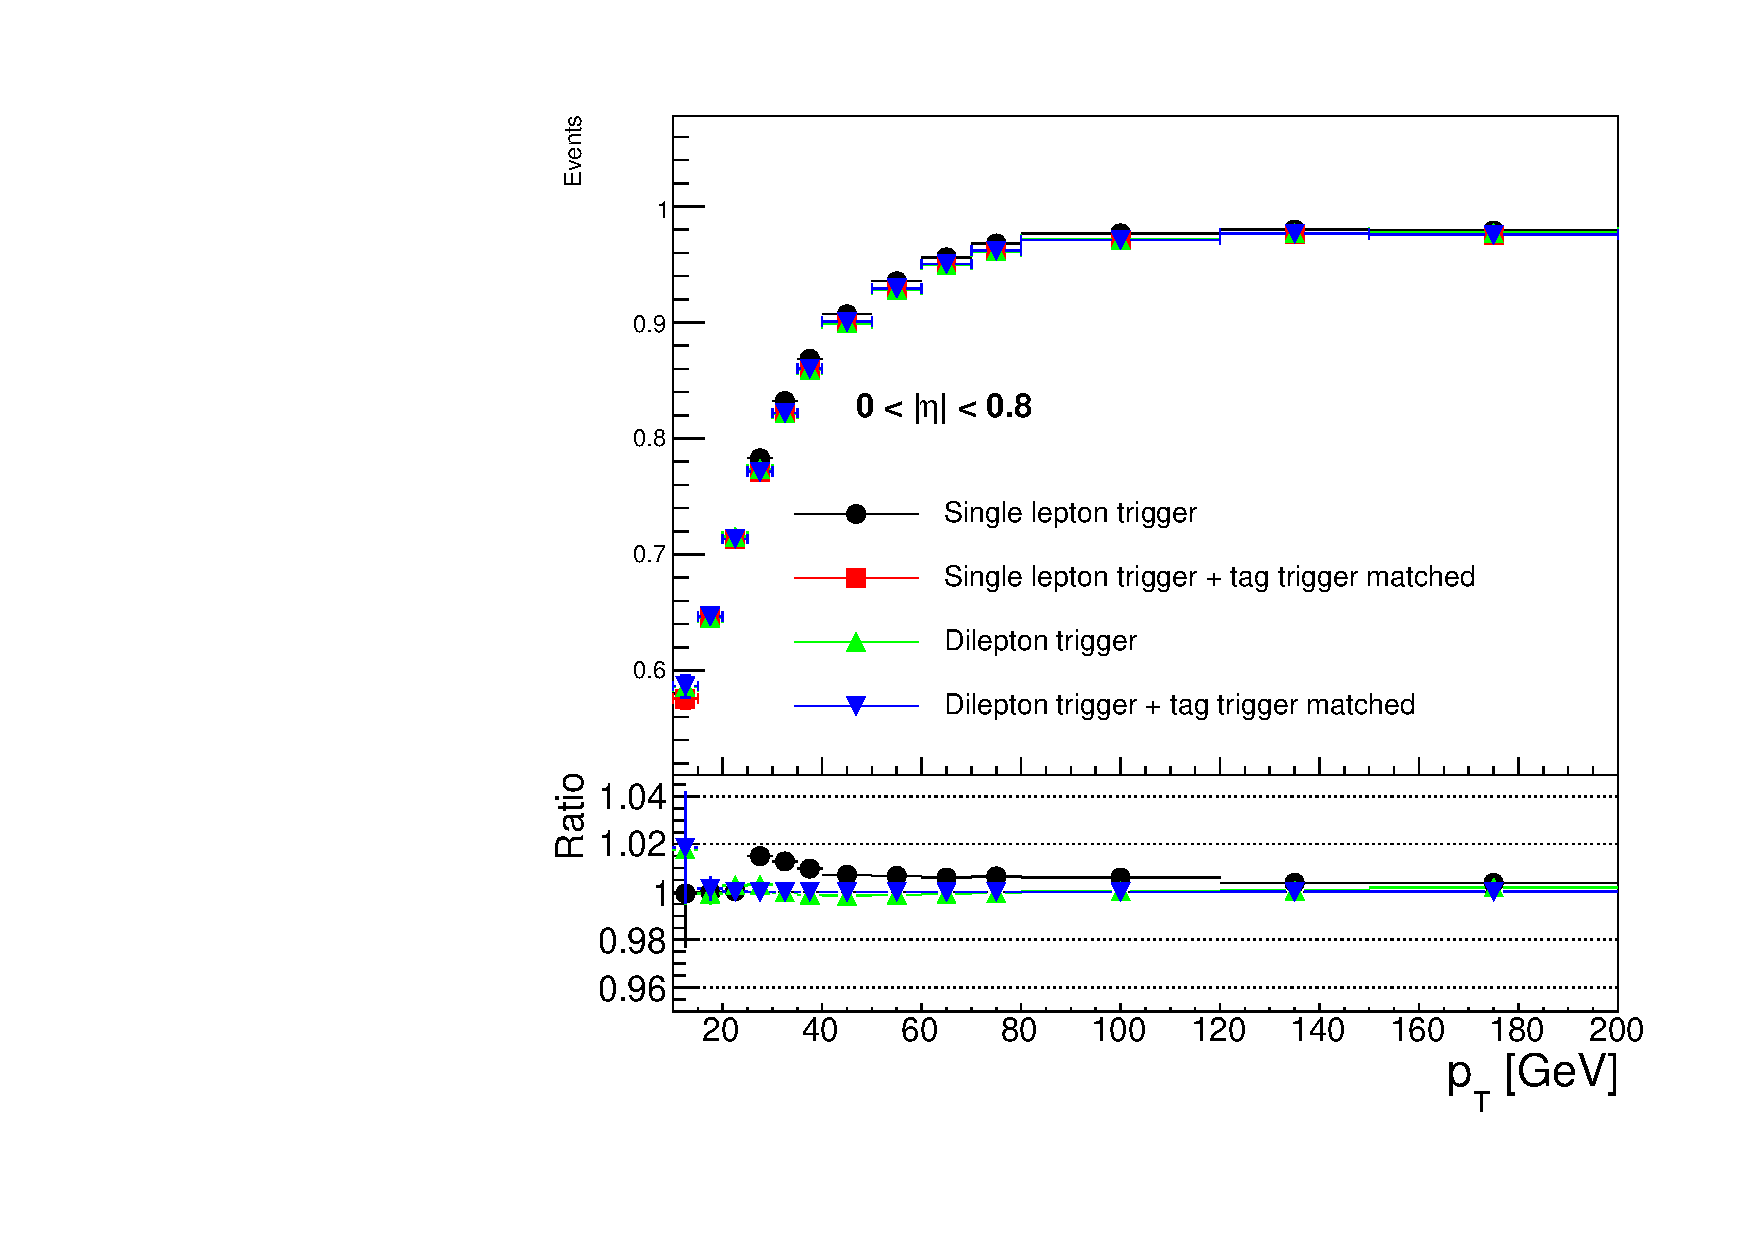
\includegraphics[scale=0.25]{trigger_uncertainty_electron_eta080_ratio_plot.pdf}
            \caption{$0 < |\eta| < 0.8$}
        \end{center}
    \end{subfigure}
    \begin{subfigure}[b]{0.32\textwidth}
        \begin{center}
            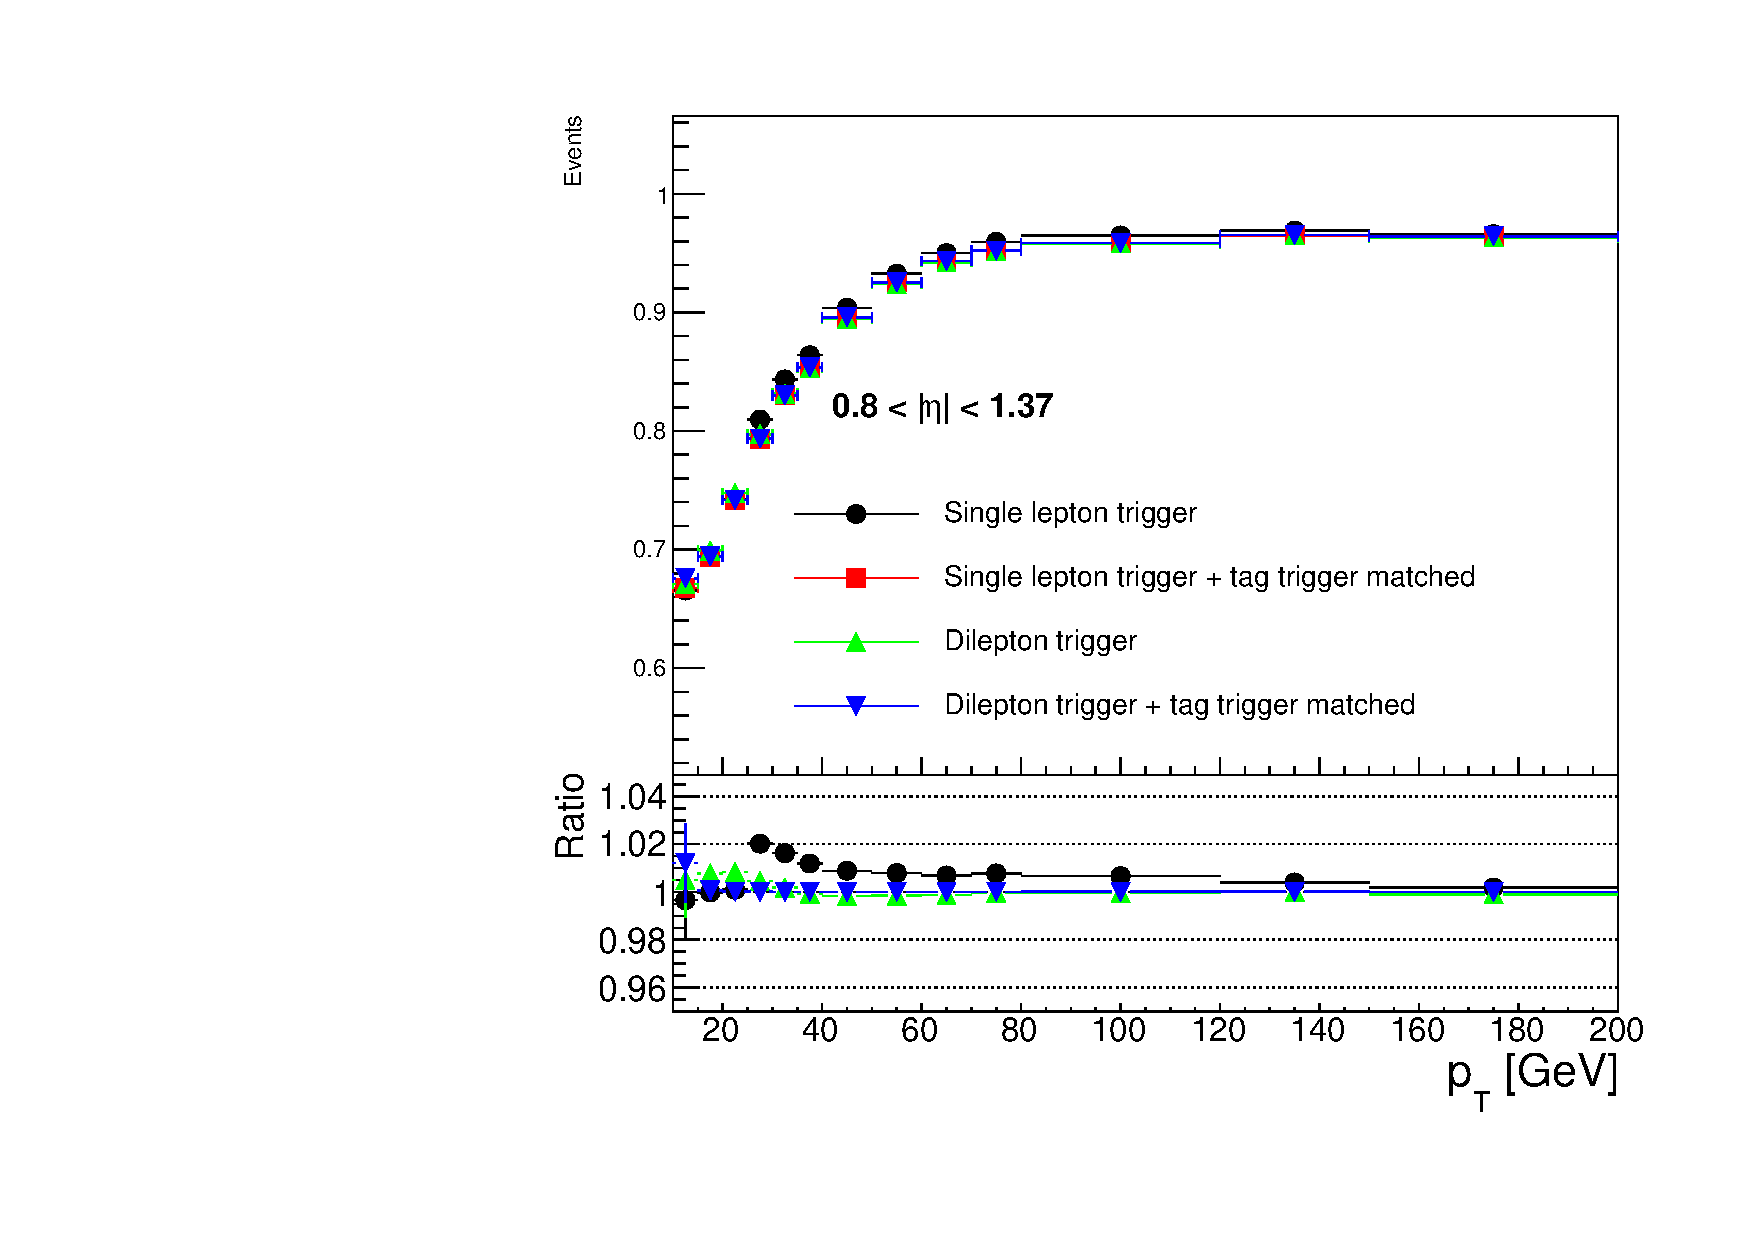
\includegraphics[scale=0.25]{trigger_uncertainty_electron_eta80137_ratio_plot.pdf}
            \caption{$0.8 < |\eta| < 1.37$}
        \end{center}
    \end{subfigure}
    \begin{subfigure}[b]{0.32\textwidth}
        \begin{center}
            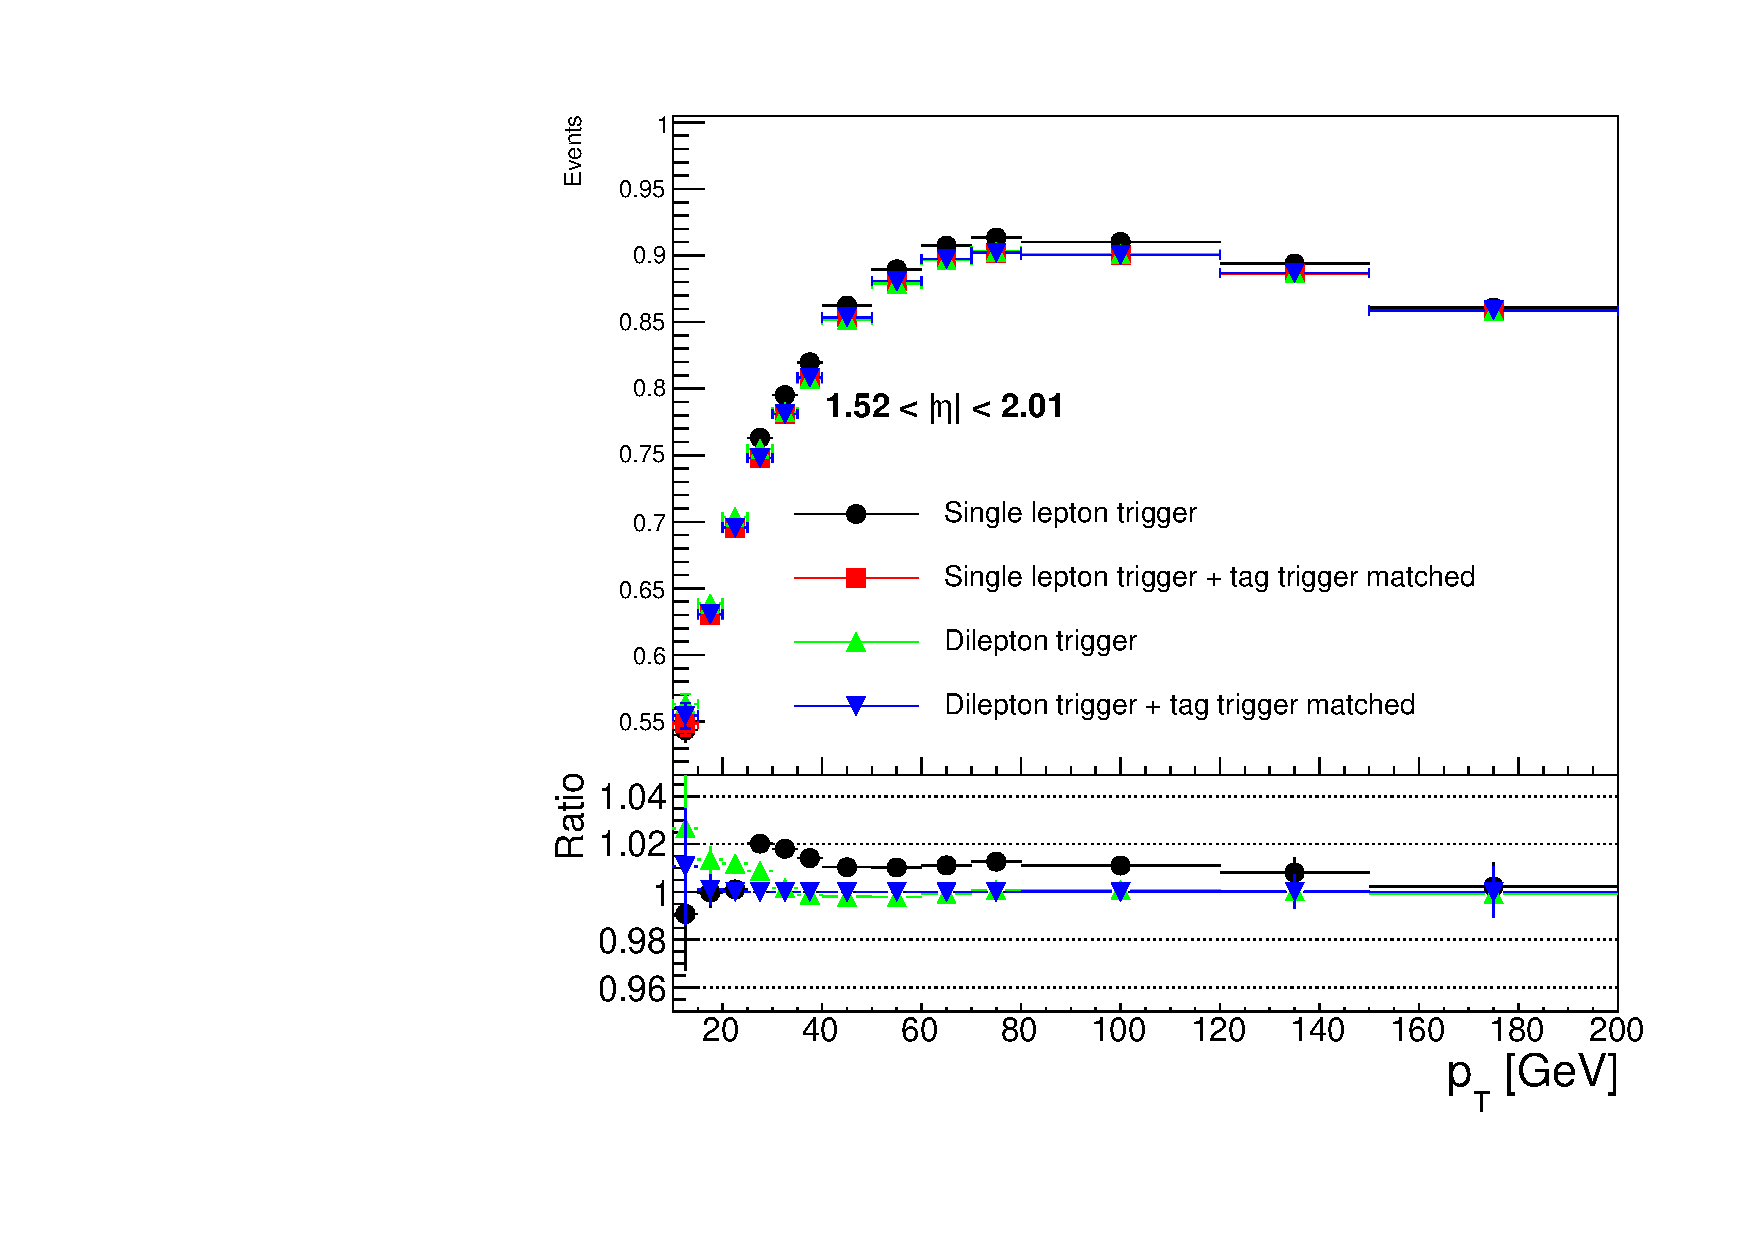
\includegraphics[scale=0.25]{trigger_uncertainty_electron_eta152201_ratio_plot.pdf}
            \caption{$1.52 < |\eta| < 2.01$}
        \end{center}
    \end{subfigure}
    \caption{The real electron efficiencies as a function of \pt in 3 $|\eta|$ regions.
    Four different trigger strategies are applied.
    The nominal values are obtained using the single lepton trigger with tag trigger matched.
    The differences between the nominal values and the values measured using other strategies are assigned as the systematic uncertainties.}
    \label{fig:app_RLE_trigger_bias_electron}
\end{figure}

\begin{figure}[htbp]
    \begin{subfigure}[b]{0.48\textwidth}
        \begin{center}
            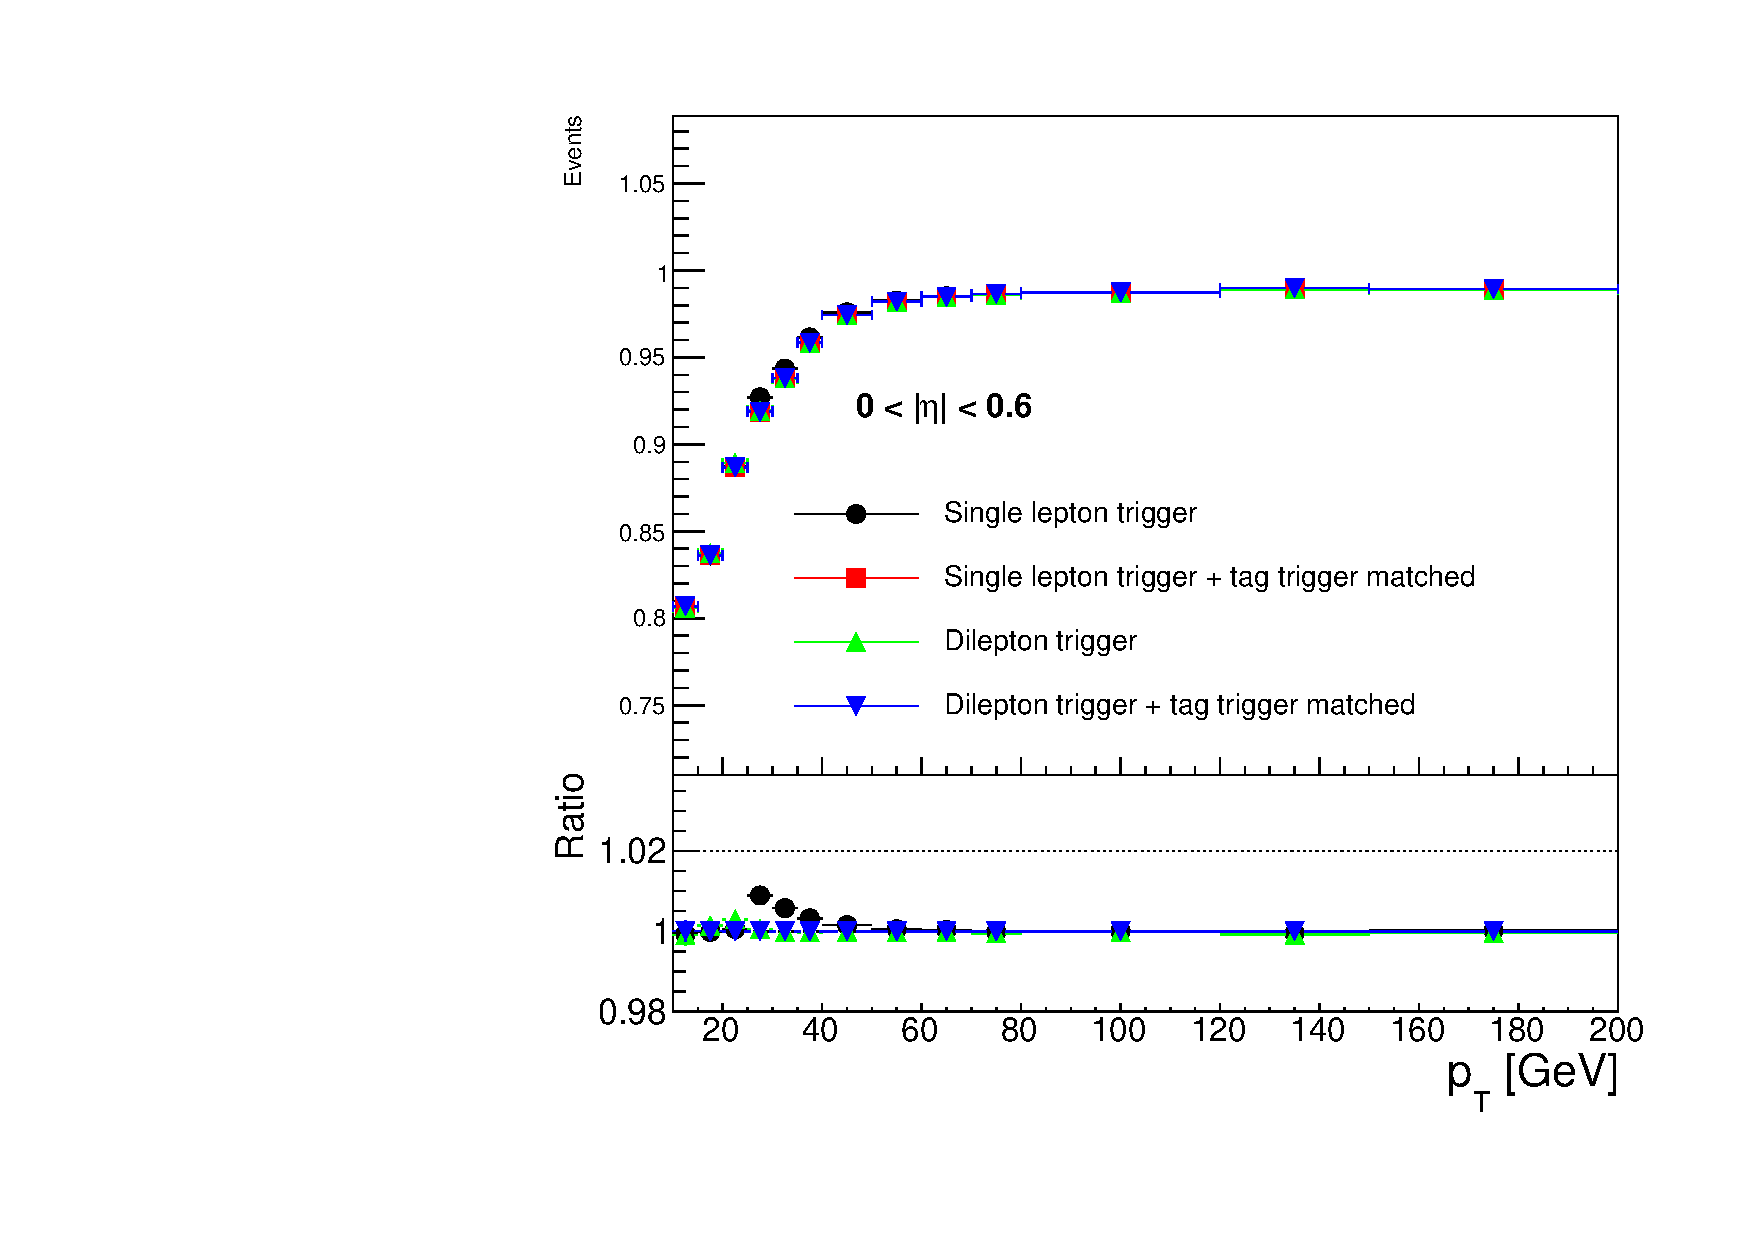
\includegraphics[scale=0.35]{trigger_uncertainty_muon_eta060_ratio_plot.pdf}
            \caption{$0 < |\eta| < 0.6$}
        \end{center}
    \end{subfigure}
    \begin{subfigure}[b]{0.48\textwidth}
        \begin{center}
            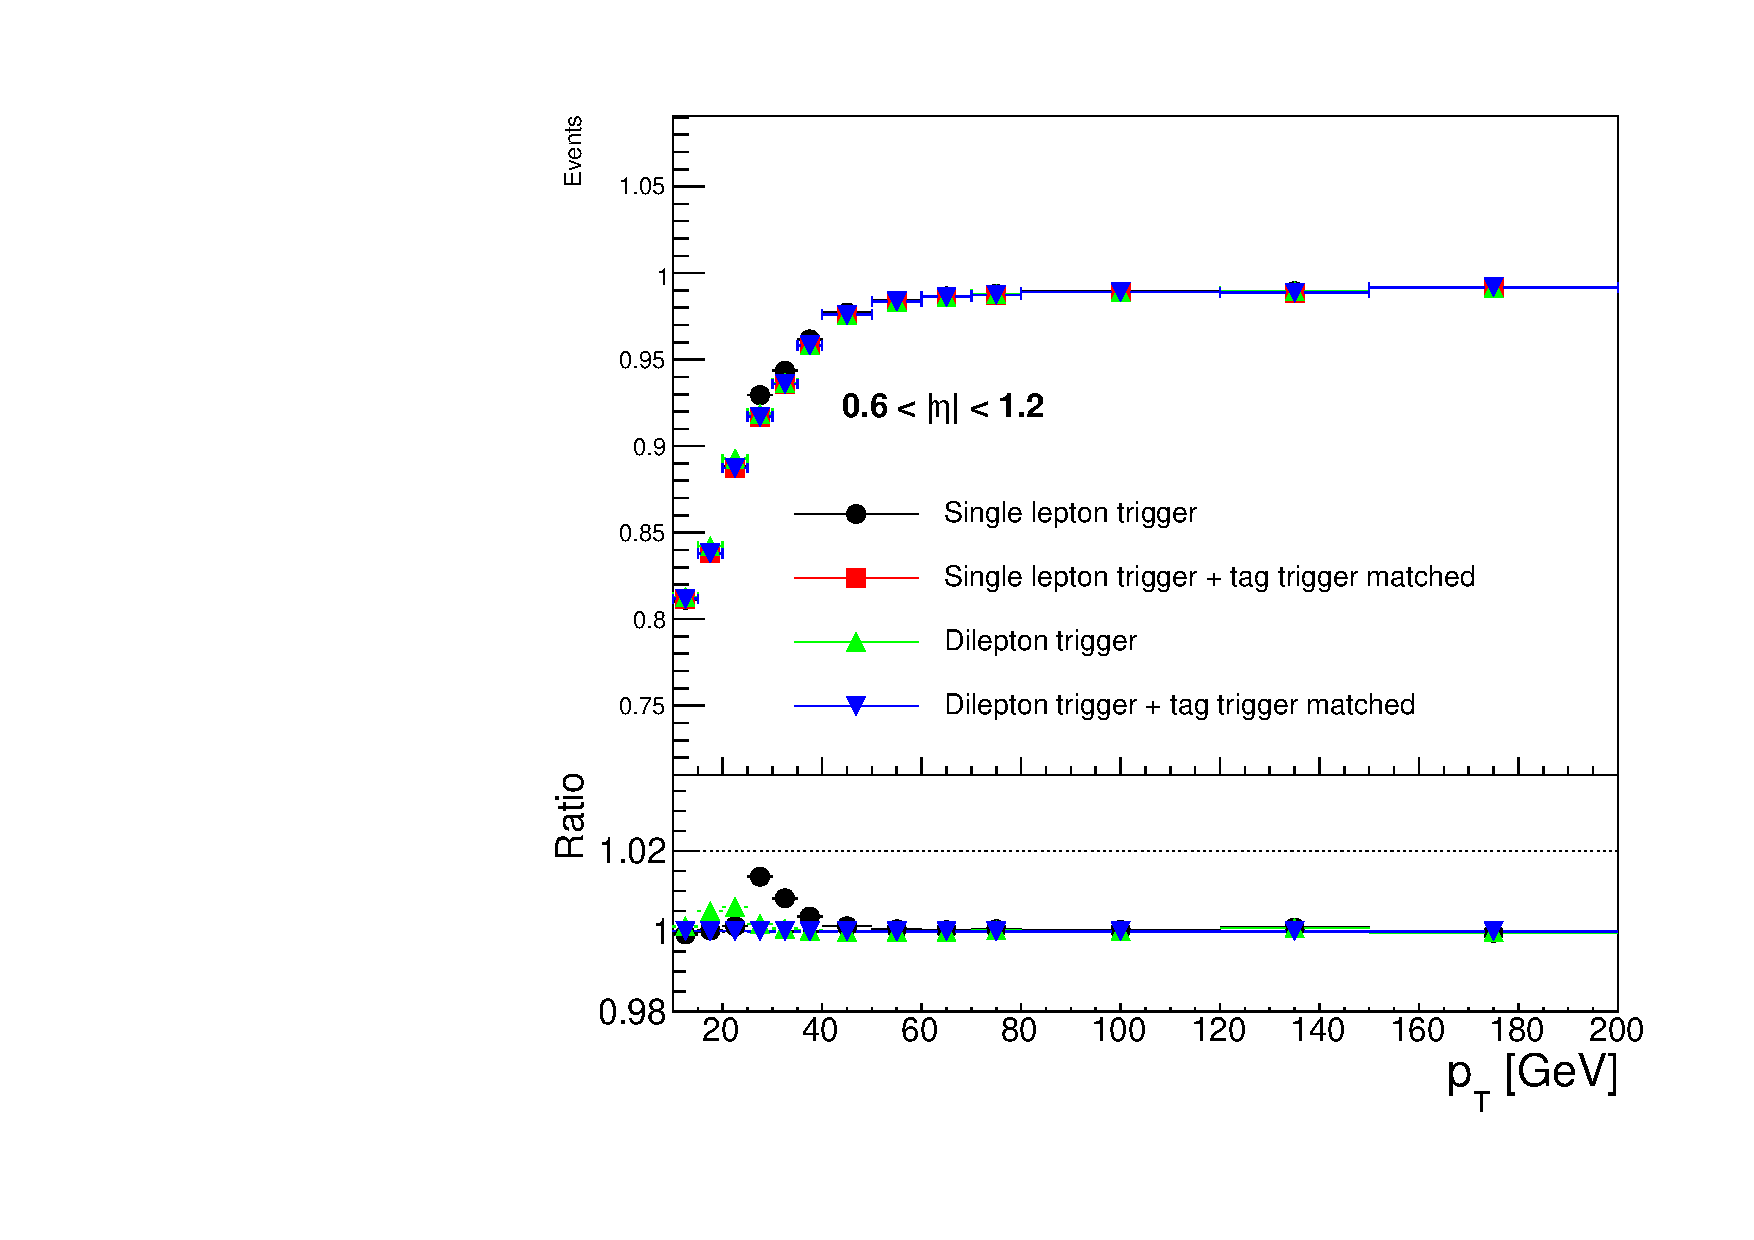
\includegraphics[scale=0.35]{trigger_uncertainty_muon_eta60120_ratio_plot.pdf}
            \caption{$0.6 < |\eta| < 1.2$}
        \end{center}
    \end{subfigure}
    \begin{subfigure}[b]{0.48\textwidth}
        \begin{center}
            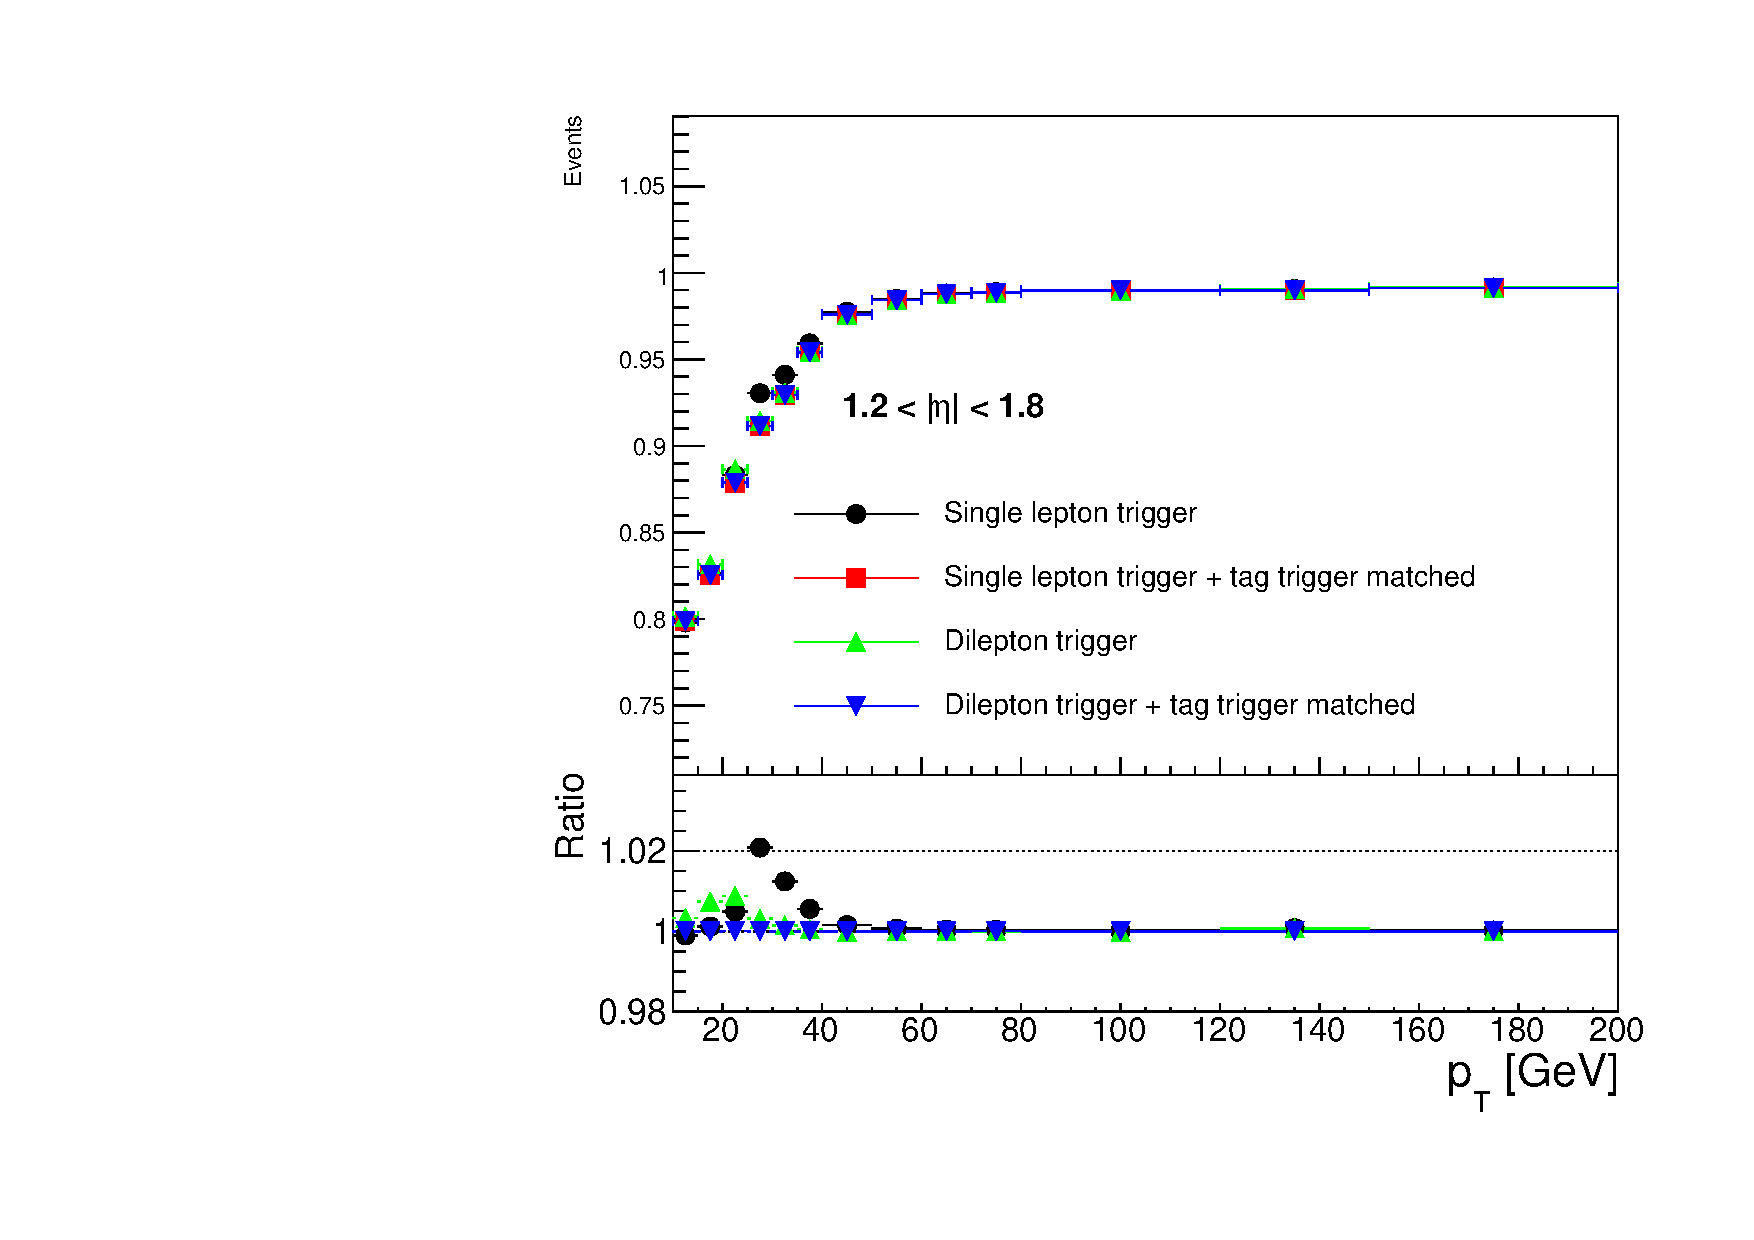
\includegraphics[scale=0.35]{trigger_uncertainty_muon_eta120180_ratio_plot.pdf}
            \caption{$1.2 < |\eta| < 1.8$}
        \end{center}
    \end{subfigure}
    \begin{subfigure}[b]{0.48\textwidth}
        \begin{center}
            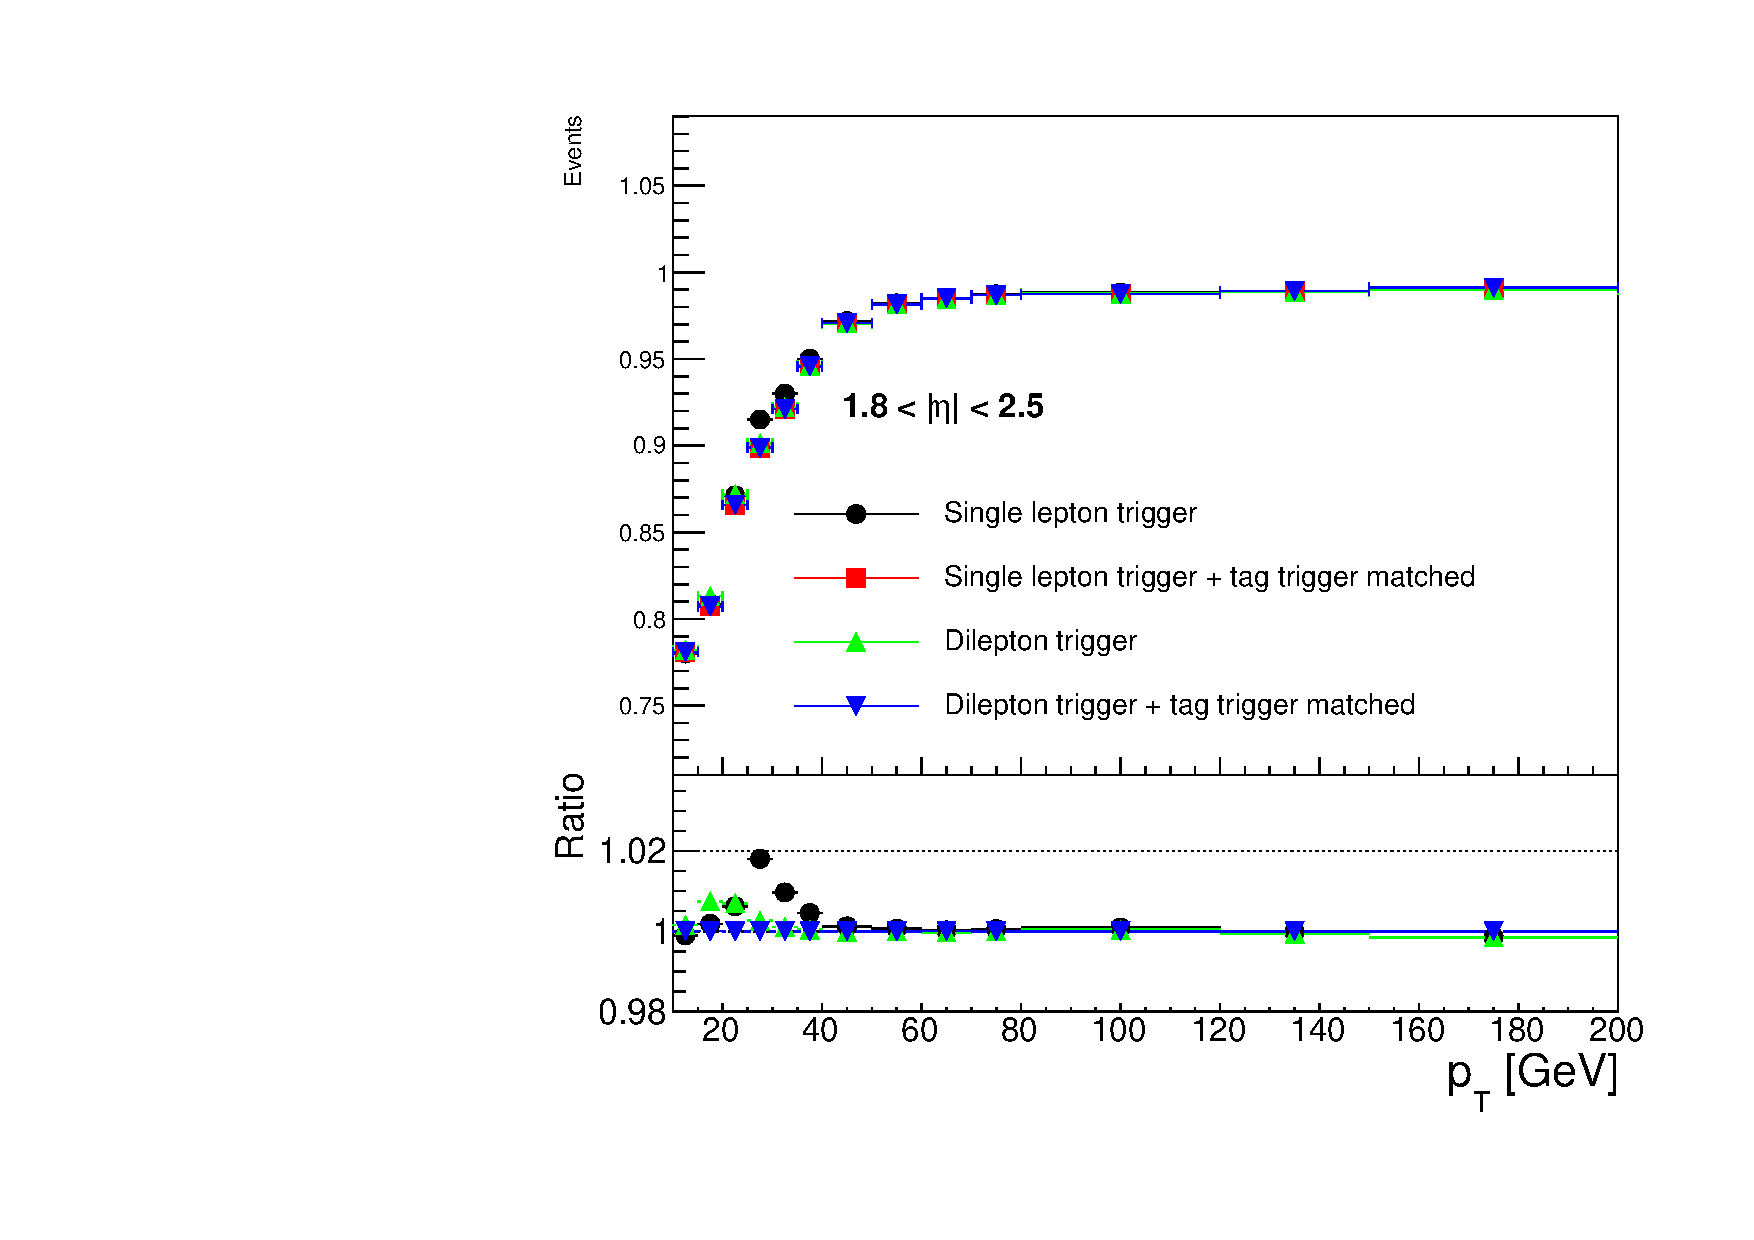
\includegraphics[scale=0.35]{trigger_uncertainty_muon_eta180250_ratio_plot.pdf}
            \caption{$1.8 < |\eta| < 2.5$}
        \end{center}
    \end{subfigure}
    \caption{The real muon efficiencies as a function of \pt in 4 $|\eta|$ regions.
    Four different trigger strategies are applied.
    The nominal values are obtained using the single lepton trigger with tag trigger matched.
    The differences between the nominal values and the values measured using other strategies are assigned as the systematic uncertainties.}
    \label{fig:app_RLE_trigger_bias_muon}
\end{figure}

\begin{table}[htbp]
    \begin{center}
        {\footnotesize
            \begin{tabular}{cccc}
                \hline
                \hline
                \multicolumn{4}{c}{Electrons (trigger)}\\
                \hline
                $|\eta|$                 & [0, 0.8] & [0.8, 1.37] & [1.52, 2.0]\\
                \hline
                $10 < \pt < 15$~{\GeV}   & 2.46\%   & 1.32\%      & 3.02\%\\
                $15 < \pt < 20$~{\GeV}   & 0.16\%   & 0.78\%      & 1.33\%\\
                $20 < \pt < 25$~{\GeV}   & 0.29\%   & 0.84\%      & 1.18\%\\
                $25 < \pt < 30$~{\GeV}   & 1.53\%   & 2.07\%      & 2.20\%\\
                $30 < \pt < 35$~{\GeV}   & 1.28\%   & 1.63\%      & 1.81\%\\
                $35 < \pt < 40$~{\GeV}   & 0.98\%   & 1.19\%      & 1.42\%\\
                $40 < \pt < 50$~{\GeV}   & 0.73\%   & 0.90\%      & 1.05\%\\
                $50 < \pt < 60$~{\GeV}   & 0.68\%   & 0.81\%      & 1.05\%\\
                $60 < \pt < 70$~{\GeV}   & 0.61\%   & 0.70\%      & 1.13\%\\
                $70 < \pt < 80$~{\GeV}   & 0.65\%   & 0.77\%      & 1.27\%\\
                $80 < \pt < 120$~{\GeV}  & 0.60\%   & 0.66\%      & 1.11\%\\
                $120 < \pt < 120$~{\GeV} & 0.38\%   & 0.40\%      & 0.79\%\\
                $150 < \pt < 200$~{\GeV} & 0.43\%   & 0.22\%      & 0.25\%\\
                \hline
                \hline
            \end{tabular}
        }
    \end{center}
    \caption{The systematic uncertainties for real electron efficiencies due to the different trigger strategies.
    The uncertainties of each trigger strategy are calculated with respect to the one applied single lepton trigger with tag trigger matched.
    The total uncertainties are the quadratic sum of the uncertainties of each trigger strategy.}
    \label{tab:app_RLE_trigger_syst_elec}
\end{table}

\begin{table}[htbp]
    \begin{center}
        {\footnotesize
            \begin{tabular}{ccccc}
                \hline
                \hline
                \multicolumn{5}{c}{Muons (trigger)}\\
                \hline
                $|\eta|$                 & [0, 0.6] & [0.6, 1.2] & [1.2, 1.8] & [1.8, 2.5]\\
                \hline
                $10 < \pt < 15$~{\GeV}   & 0.11\%   & 0.15\%     & 0.34\%     & 0.19\%\\
                $15 < \pt < 20$~{\GeV}   & 0.14\%   & 0.50\%     & 0.75\%     & 0.77\%\\
                $20 < \pt < 25$~{\GeV}   & 0.30\%   & 0.63\%     & 1.01\%     & 0.93\%\\
                $25 < \pt < 30$~{\GeV}   & 0.90\%   & 1.38\%     & 2.12\%     & 1.83\%\\
                $30 < \pt < 35$~{\GeV}   & 0.58\%   & 0.84\%     & 1.27\%     & 0.99\%\\
                $35 < \pt < 40$~{\GeV}   & 0.33\%   & 0.37\%     & 0.57\%     & 0.46\%\\
                $40 < \pt < 50$~{\GeV}   & 0.16\%   & 0.13\%     & 0.16\%     & 0.13\%\\
                $50 < \pt < 60$~{\GeV}   & 0.06\%   & 0.06\%     & 0.07\%     & 0.07\%\\
                $60 < \pt < 70$~{\GeV}   & 0.04\%   & 0.04\%     & 0.04\%     & 0.04\%\\
                $70 < \pt < 80$~{\GeV}   & 0.05\%   & 0.06\%     & 0.04\%     & 0.06\%\\
                $80 < \pt < 120$~{\GeV}  & 0.03\%   & 0.03\%     & 0.03\%     & 0.11\%\\
                $120 < \pt < 120$~{\GeV} & 0.05\%   & 0.13\%     & 0.10\%     & 0.08\%\\
                $150 < \pt < 200$~{\GeV} & 0.04\%   & 0.03\%     & 0.02\%     & 0.19\%\\
                \hline
                \hline
            \end{tabular}
        }
    \end{center}
    \caption{The systematic uncertainties for real muon efficiencies due to the different trigger strategies.
    The uncertainties of each trigger strategy are calculated with respect to the one applied single lepton trigger with tag trigger matched.
    The total uncertainties are the quadratic sum of the uncertainties of each trigger strategy.}
    \label{tab:app_RLE_trigger_syst_muon}
\end{table}

%%%
%%%
%%%

\subsection{Extrapolation to signal regions}
\label{subsec:app_RLE_extrapolation_to_signal_region}
Because $Z\to \ell\ell$ events are characterized by well isolated leptons, the leptons presented in the final state are not necessary well isolated using different processes.
The processes other than $Z\to \ell\ell$ might contain many ($b$-)jets in the SR and with different event topologies.
In order to study different event topologies, a SUSY benchmark model $\tilde{g}\to\ttbar \widetilde{\chi}^{0}_{1}$ is used and $\Delta m = m_{\tilde{g}} - m_{\chi^{0}_{1}} > 1$~{\TeV} requirement is applied on the model to selected boosted event.
Since one of the main irreducible background, $\ttbar V$, has similar event topology, the \ttbar samples are also considered.
The difference in the real lepton efficiencies between the two processes are assigned as system uncertainties.
Figure~\ref{fig:app_RLE_kinematic} shows the kinematic distributions of the baseline leptons for $Z\to \ell\ell$, $\tilde{g} \to \ttbar \widetilde{\chi}^{0}_{1}$, and \ttbar processes.

\begin{figure}[htb]
    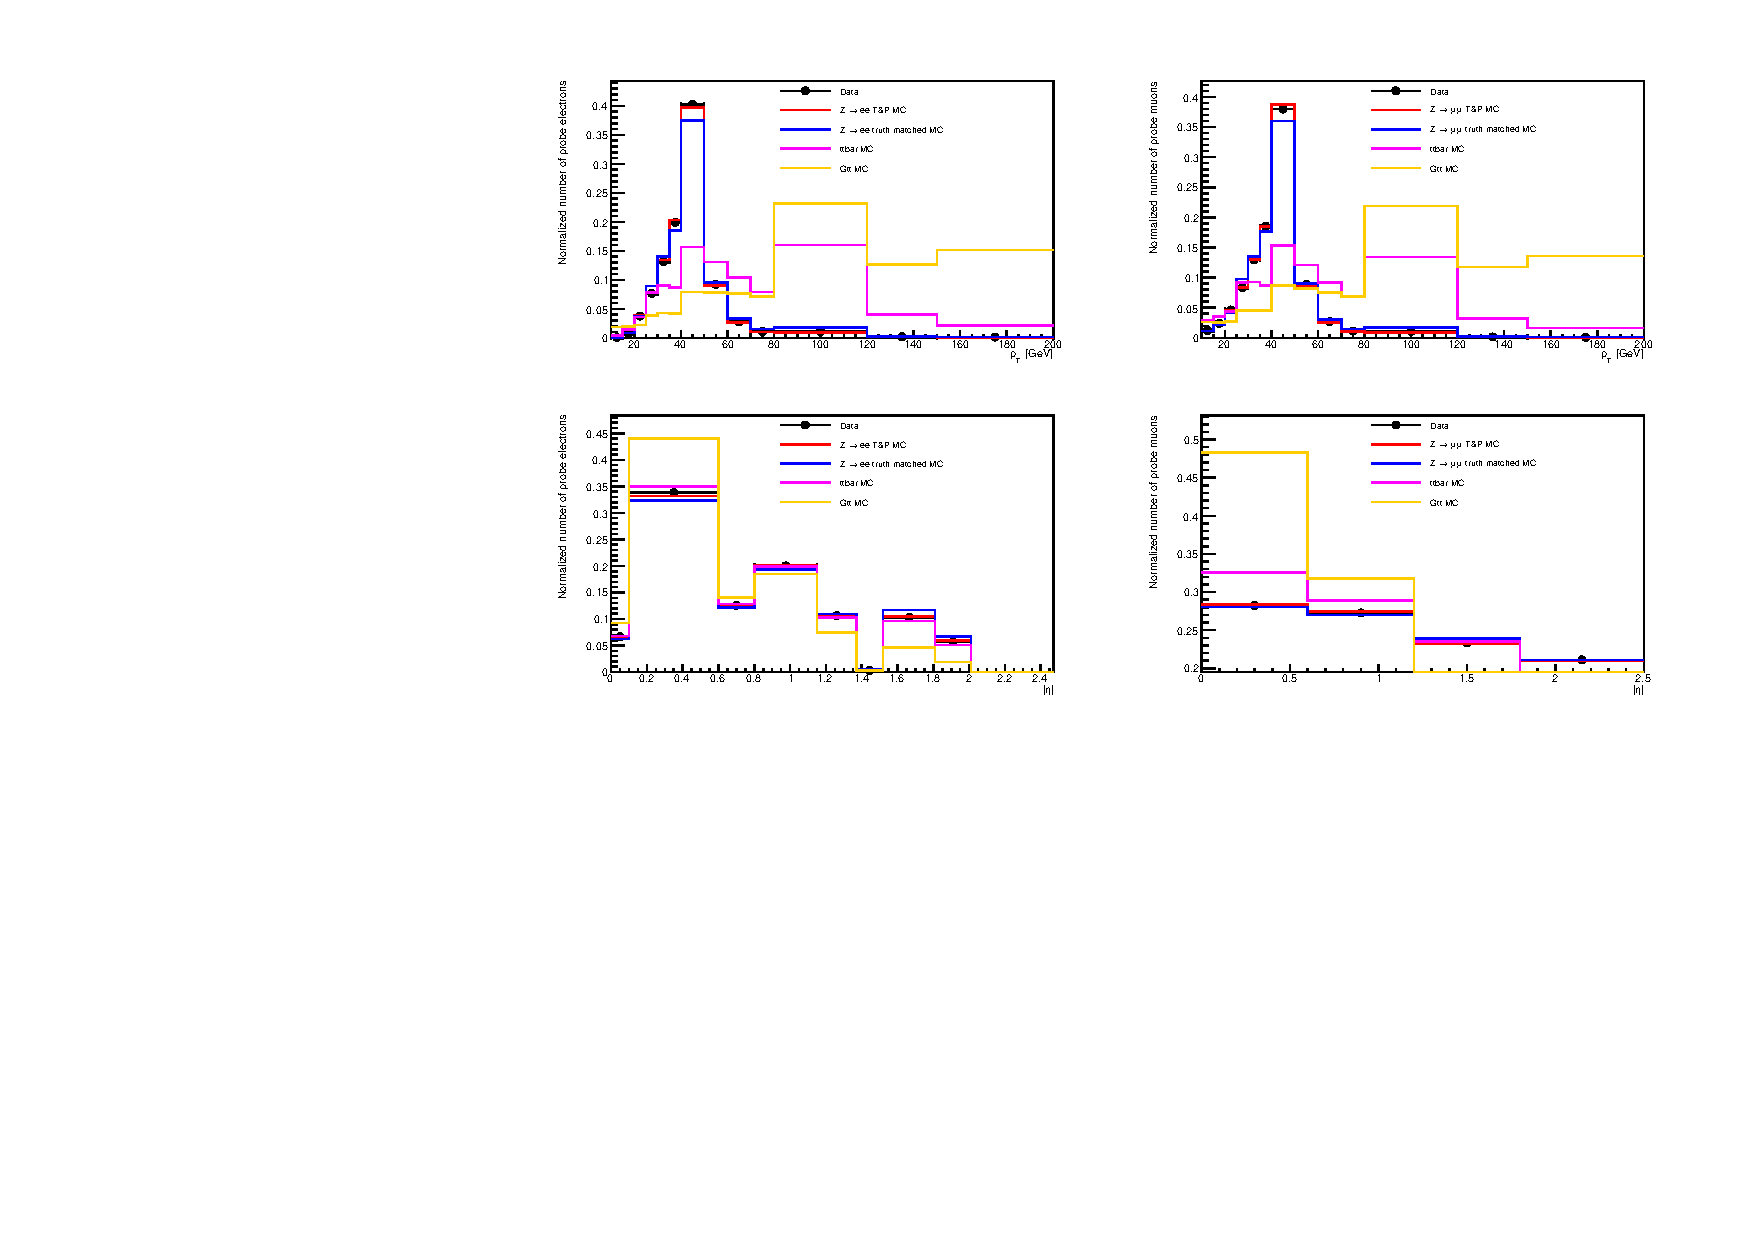
\includegraphics[width=0.96\textwidth]{baseline_kinematics.pdf}
    \caption{The kinematic distributions of the baseline leptons for $Z\to \ell\ell$, $\tilde{g} \to \ttbar \widetilde{\chi}^{0}_{1}$, and \ttbar processes.
    The top row is the \pt distributions and the bottom row is the $|\eta|$ distributions.
    The electron case is on the left hand side and the muon case is on the right hand side.
    The $\tilde{g} \to \ttbar \widetilde{\chi}^{0}_{1}$ process is more boosted and centralized than the $Z\to \ell \ell$ and \ttbar processes.}
    \label{fig:app_RLE_kinematic}
\end{figure}

The SUSY process $\tilde{g} \to \ttbar \widetilde{\chi}^{0}_{1}$ is more boosted and centralized than the $Z\to \ell \ell$ and \ttbar processes.
Figure~\ref{fig:app_RLE_dRjet_Njet} shows the $\Delta R(\ell, \mathrm{jet})$ and the $N_\mathrm{jets}$ distributions of the baseline leptons for $Z\to \ell\ell$, $\tilde{g} \to \ttbar \widetilde{\chi}^{0}_{1}$, and \ttbar processes.
The leptons from the $Z \to \ell \ell$ processes are not accompanied with a signal jet and the $\Delta R(\ell, \mathrm{jet})$ distribution peak about $\Delta R(\ell, \mathrm{jet}) = 3$.
The leptons from the SUSY process $\tilde{g} \to \ttbar \widetilde{\chi}^{0}_{1}$ peak at $\Delta R(\ell, \mathrm{jet}) = 0.5$ and most of the statistics are located in $\Delta R(\ell, \mathrm{jet}) < 1$ region.
The $Z \to \ell \ell$ peaks at $N_\mathrm{jets} = 4$ and $N_\mathrm{jets} = 3$ for the electron and muon case, respectively.
The SUSY process $\tilde{g} \to \ttbar \widetilde{\chi}^{0}_{1}$ peaks at $N_\mathrm{jets} = 9$.
Hence, the leptons produced in the SUSY process are accompanied with many jets and less isolated than the $Z \to \ell \ell$ process.
If the isolation requirement is looser, then the associated real lepton efficiencies are larger.
This extreme topology enables us to assess a conservative SUSY signal extrapolation systematic uncertainty that should cover all SUSY signal processes considered by the analysis.

\begin{figure}[htb]
    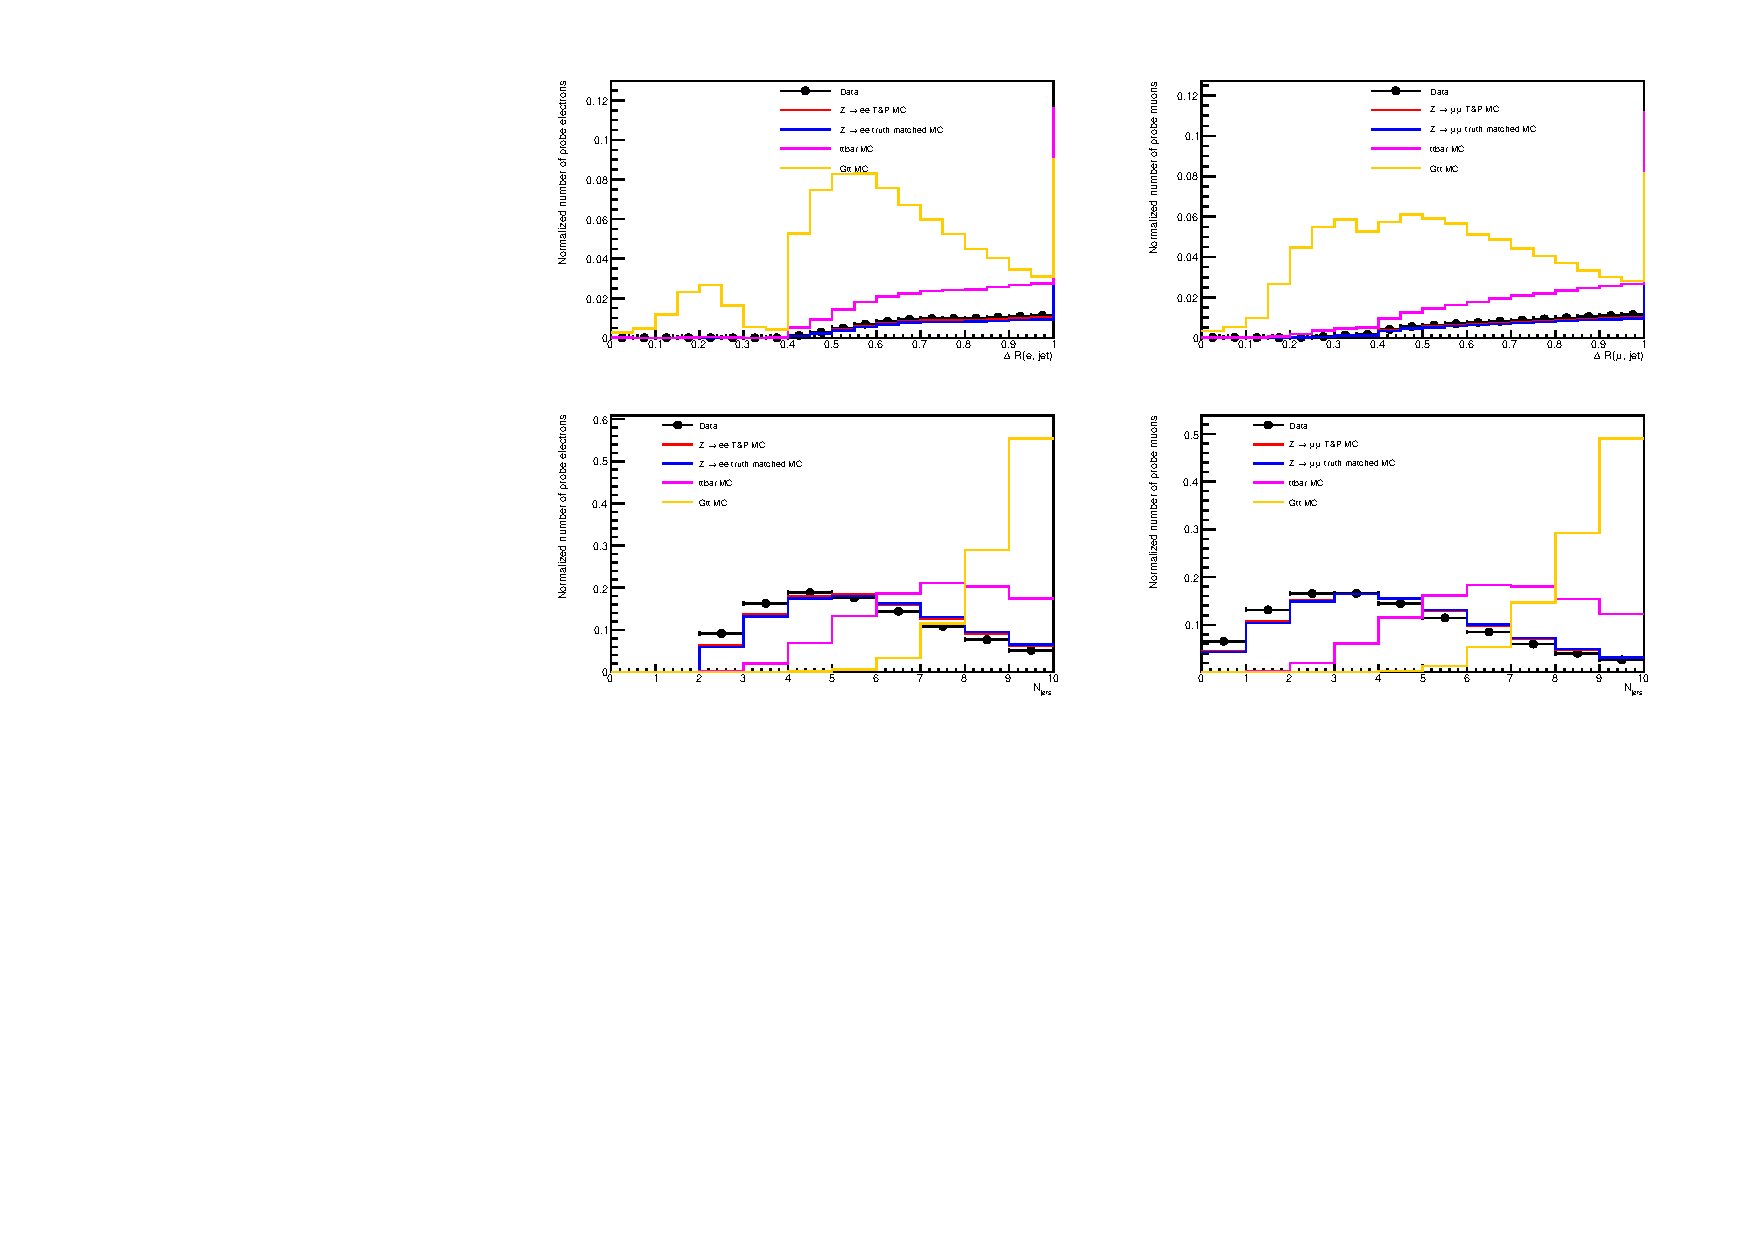
\includegraphics[width=0.96\textwidth]{baseline_deltaR_and_NJets.pdf}
    \caption{The $\Delta R(\ell, \mathrm{jet})$ and the $N_\mathrm{jets}$ distributions of the baseline leptons for $Z\to \ell\ell$, $\tilde{g} \to \ttbar \widetilde{\chi}^{0}_{1}$, and \ttbar processes.
    The top row is the $\Delta R(\ell, \mathrm{jet})$ distributions and the bottom row is the $N_\mathrm{jets}$ distributions.
    The electron case is on the left hand side and the muon case is on the right hand side.
    The statistics of $Z \to \ell \ell$ processes are populated at higher $\Delta R(\ell, \mathrm{jet}) < 1$ region and lower $N_\mathrm{jets}$ region.
    The statistics of $\tilde{g} \to \ttbar \widetilde{\chi}^{0}_{1}$ are located in $\Delta R(\ell, \mathrm{jet}) < 1$ region and higher $N_\mathrm{jets}$ region.}
    \label{fig:app_RLE_dRjet_Njet}
\end{figure}

Figure~\ref{fig:app_RLE_real_efficiency_ttbar_gtt} shows the real lepton efficiencies as a function of \pt using $Z\to \ell\ell$, $\tilde{g} \to \ttbar \widetilde{\chi}^{0}_{1}$, and \ttbar processes and the ratio with respect to the data is shown in the lower panel.
The real electron efficiencies are \pt dependent when $\pt < 50$~{\GeV} and become stable when $ \pt > 50$~{\GeV}.
The real electron efficiencies of $\tilde{g} \to \ttbar \widetilde{\chi}^{0}_{1}$ are $\sim$8\% lower than the efficiencies of $Z \to ee$.
The observed differences in the low \pt region are mostly due to the calorimeter isolation and the track isolation requirements.
The differences in the real muon efficiencies mainly come from the track isolation and $d_{0}/\sigma_{d_{0}}$ requirements.
The average efficiencies of $Z \to \ell \ell$ are computed and the relative efficiency differences are calculated  with respect to the average efficiencies.
Table~\ref{tab:app_RLE_syst_busy} shows the relative efficiency differences as a function of $\Delta R(\ell, jet)$ in  \pt bins.

\begin{table}[htb]
    \resizebox{\textwidth}{!}{%
        {\footnotesize
            \begin{tabular}{ccccccccc}
                \hline
                \hline
                \multicolumn{9}{c}{electrons (busy environments)}\\
                \hline
                $\Delta R(e, \mathrm{jet})$ & [0, 0.1] & [0.1, 0.15] & [0.15, 0.2] & [0.2, 0.3] & [0.3, 0.35] & [0.35, 0.4] & [0.4, 0.6] & [0.6, 4]\\
                \hline
                $10 < \pt < 20$~{\GeV}      & -        & -           & -           & -          & -           & -           & 25.31\%    & 6.5\%\\
                $20 < \pt < 30$~{\GeV}      & -        & -           & -           & -          & -           & 73.37\%     & 10.21\%    & 0.37\%\\
                $30 < \pt < 40$~{\GeV}      & -        & -           & -           & 97.71\%    & 48.22\%     & 15.54\%     & 7.29\%     & 0.58\%\\
                $40 < \pt < 50$~{\GeV}      & -        & -           & -           & 52.81\%    & 22.80\%     & 16.73\%     & 7.68\%     & 1.10\%\\
                $50 < \pt < 60$~{\GeV}      & -        & -           & -           & 29.96\%    & 21.49\%     & 20.23\%     & 6.99\%     & 2.78\%\\
                $60 < \pt < 80$~{\GeV}      & -        & -           & 55.89\%     & 24.31\%    & 17.40\%     & 24.77\%     & 6.20\%     & 2.87\%\\
                $80 < \pt < 150$~{\GeV}     & -        & 57.52\%     & 30.24\%     & 16.45\%    & 12.73\%     & 20.92\%     & 4.44\%     & 2.73\%\\
                $150 < \pt < 200$~{\GeV}    & 88.54\%  & 40.16\%     & 19.34\%     & 8.45\%     & 14.66\%     & 16.57\%     & 2.57\%     & 1.90\%\\
                \hline
                \hline
                \multicolumn{9}{c}{muons (busy environments)}\\
                \hline
                $\Delta R(\mu, \mathrm{jet})$ & [0, 0.1] & [0.1, 0.15] & [0.15, 0.2] & [0.2, 0.3] & [0.3, 0.35] & [0.35, 0.4] & [0.4, 0.6] & [0.6, 4]\\
                \hline
                $10 < \pt < 20$~{\GeV}        & -        & -           & -           & -          & -           & -           & 33.59\%    & 5.18\%\\
                $20 < \pt < 30$~{\GeV}        & -        & -           & -           & -          & -           & 82.34\%     & 22.27\%    & 3.39\%\\
                $30 < \pt < 40$~{\GeV}        & -        & -           & -           & 98.54\%    & 56.36\%     & 31.89\%     & 14.22\%    & 2.24\%\\
                $40 < \pt < 50$~{\GeV}        & -        & -           & -           & 53.10\%    & 21.33\%     & 13.90\%     & 6.81\%     & 1.45\%\\
                $50 < \pt < 60$~{\GeV}        & -        & -           & -           & 24.98\%    & 13.72\%     & 9.62\%      & 3.83\%     & 0.79\%\\
                $60 < \pt < 80$~{\GeV}        & -        & -           & 44.41\%     & 13.75\%    & 6.14\%      & 4.76\%      & 2.04\%     & 0.15\%\\
                $80 < \pt < 150$~{\GeV}       & -        & 29.94\%     & 7.14\%      & 3.16\%     & 1.30\%      & 1.04\%      & 0.07\%     & 0.57\%\\
                $150 < \pt < 200$~{\GeV}      & 82.26\%  & 4.14\%      & 1.02\%      & 0.17\%     & 0.29\%      & 0.62\%      & 1.02\%     & 1.13\%\\
                \hline
                \hline
            \end{tabular}
        }
    }
    \caption{The systematic uncertainties of the real lepton efficiency in busy environment using $\tilde{g} \to \ttbar \widetilde{\chi_1^0}$.}
    \label{tab:app_RLE_syst_busy}
\end{table}

%%%
%%%
%%%

\subsection{Final uncertainties}
\label{subsec:app_RLE_final_uncertainties}
The final uncertainties are the quadratic sum of the statistical uncertainties and the systematic uncertainties.
The sources of systematic uncertainty include the measurement uncertainty, the trigger uncertainty, the uncertainty from the differences between $Z$ tag-and-probe method and truth matching, and the uncertainty in the busy environment.
Table~\ref{tab:app_RLE_syst_busy} shows the uncertainty in the busy environment.
The uncertainty in the busy environment is measured as a function of \pT and $\Delta R$ so it doesn't combine with the other uncertainties which are function of \pT and $|\eta|$.
Table~\ref{tab:app_RLE_final_uncertainties_elec} and Table~\ref{tab:app_RLE_final_uncertainties_muon} show the final uncertainties for electron and muon real efficiencies, respectively.

\begin{table}[htb]
    \begin{center}
        {\footnotesize
            \begin{tabular}{cccc}
                \hline
                \hline
                \multicolumn{4}{c}{Electrons (final uncertainties)}\\
                \hline
                $|\eta|$                 & [0, 0.8] & [0.8, 1.37] & [1.52, 2.0]\\
                \hline
                $10 < \pt < 15$~{\GeV}   & 0.047    & 0.063       & 0.089\\
                $15 < \pt < 20$~{\GeV}   & 0.027    & 0.042       & 0.062\\
                $20 < \pt < 25$~{\GeV}   & 0.018    & 0.031       & 0.041\\
                $25 < \pt < 30$~{\GeV}   & 0.029    & 0.024       & 0.027\\
                $30 < \pt < 35$~{\GeV}   & 0.023    & 0.021       & 0.023\\
                $35 < \pt < 40$~{\GeV}   & 0.014    & 0.018       & 0.018\\
                $40 < \pt < 50$~{\GeV}   & 0.007    & 0.010       & 0.010\\
                $50 < \pt < 60$~{\GeV}   & 0.008    & 0.010       & 0.010\\
                $60 < \pt < 70$~{\GeV}   & 0.007    & 0.010       & 0.010\\
                $70 < \pt < 80$~{\GeV}   & 0.008    & 0.011       & 0.012\\
                $80 < \pt < 120$~{\GeV}  & 0.010    & 0.010       & 0.011\\
                $120 < \pt < 120$~{\GeV} & 0.005    & 0.005       & 0.011\\
                $150 < \pt < 200$~{\GeV} & 0.005    & 0.003       & 0.020\\
                \hline
                \hline
            \end{tabular}
        }
    \end{center}
    \caption{The final uncertainties of the real electron efficiencies.
    The final uncertainties are the quadratic sum of the statistical uncertainties and the systematic uncertainties.
    The systematic uncertainties include the measurement uncertainty, the trigger uncertainty, the uncertainty comes from the differences between $Z$ tag-and-probe method and truth matching.
    The uncertainties in the busy environment do not incorporate in the final uncertainties calculation because it is measured as a function of \pT and $\Delta R$.
    The trigger uncertainties are measured using $\pT > 20$~{\GeV} only.}
    \label{tab:app_RLE_final_uncertainties_elec}
\end{table}

\begin{table}[htb]
    \begin{center}
        {\footnotesize
            \begin{tabular}{ccccc}
                \hline
                \hline
                \multicolumn{5}{c}{Muons (final uncertainties)}\\
                \hline
                $|\eta|$                 & [0, 0.6] & [0.6, 1.2] & [1.2, 1.8] & [1.8, 2.5]\\
                \hline
                $10 < \pt < 15$~{\GeV}   & 0.014    & 0.010      & 0.008      & 0.011\\
                $15 < \pt < 20$~{\GeV}   & 0.005    & 0.006      & 0.008      & 0.011\\
                $20 < \pt < 25$~{\GeV}   & 0.003    & 0.006      & 0.010      & 0.010\\
                $25 < \pt < 30$~{\GeV}   & 0.011    & 0.015      & 0.022      & 0.019\\
                $30 < \pt < 35$~{\GeV}   & 0.007    & 0.009      & 0.014      & 0.011\\
                $35 < \pt < 40$~{\GeV}   & 0.004    & 0.004      & 0.006      & 0.006\\
                $40 < \pt < 50$~{\GeV}   & 0.002    & 0.001      & 0.002      & 0.001\\
                $50 < \pt < 60$~{\GeV}   & 0.001    & 0.001      & 0.001      & 0.001\\
                $60 < \pt < 70$~{\GeV}   & 0.001    & 0.001      & 0.001      & 0.002\\
                $70 < \pt < 80$~{\GeV}   & 0.002    & 0.001      & 0.001      & 0.002\\
                $80 < \pt < 120$~{\GeV}  & 0.004    & 0.002      & 0.002      & 0.002\\
                $120 < \pt < 120$~{\GeV} & 0.006    & 0.005      & 0.005      & 0.005\\
                $150 < \pt < 200$~{\GeV} & 0.005    & 0.005      & 0.005      & 0.006\\
                \hline
                \hline
            \end{tabular}
        }
    \end{center}
    \caption{The final uncertainties of the real muon efficiencies.
    The final uncertainties are the quadratic sum of the statistical uncertainties and the systematic uncertainties.
    The systematic uncertainties include the measurement uncertainty, the trigger uncertainty, the uncertainty comes from the differences between $Z$ tag-and-probe method and truth matching.
    The uncertainties in the busy environment do not incorporate in the final uncertainties calculation because it is measured as a function of \pT and $\Delta R$.}
    \label{tab:app_RLE_final_uncertainties_muon}
\end{table}
